%%% The DTCI.tex file
%%% Authors: Christopher Douglas, Christopher Schommer-Pries, and Noah Snyder

\documentclass{amsart}


%%%%%%% Standard Packages
\usepackage{amsmath}       % I think this gives me some symbols
\usepackage{amsthm}        % Does theorem stuff
\usepackage{amssymb}       % more symbols and fonts
\usepackage{amsfonts}
\usepackage[all]{xy}
\usepackage{xspace}
\usepackage{calc}



\setlength{\topskip}{0pt}
\setlength{\footskip}{30pt}
\headheight=0pt
\topmargin=0pt
\headsep=18pt
\textheight=603pt %% 792pt to page, 648 is 9in
\textwidth=420pt  %% 612pt to page, 468pt is 6.5in
\oddsidemargin=25pt
\evensidemargin=25pt

\pagestyle{plain}


%%%%%% Adds hyperlinks
\usepackage[colorlinks, linkcolor=black, citecolor=blue,
	% pagebackref,
 	%bookmarksnumbered=true
	]{hyperref}
	
	
	
%%%%%% Tikz !!! Commands and Macros %%%%%%%%%%%%%
\usepackage{tikz}
\usetikzlibrary{matrix}


%%%% These draw triple or quadruple set of arrows of length 0.5 cm
\DeclareMathOperator{\righttriplearrows} {{\; \tikz{ \foreach \y in {0, 0.1, 0.2} { \draw [-stealth] (0, \y) -- +(0.5, 0);}} \; }}
\DeclareMathOperator{\lefttriplearrows} {{\; \tikz{ \foreach \y in {0, 0.1, 0.2} { \draw [stealth-] (0, \y) -- +(0.5, 0);}} \; }}
\DeclareMathOperator{\rightquadarrows} {{\; \tikz{ \foreach \y in {0, 0.1, 0.2, 0.3} { \draw [-stealth] (0, \y) -- +(0.5, 0);}} \; }}
\DeclareMathOperator{\leftquadarrows} {{\; \tikz{ \foreach \y in {0, 0.1, 0.2, 0.3} { \draw [stealth-] (0, \y) -- +(0.5, 0);}} \; }}

%%%%%%% End TikZ Commands and Macros %%%%%%%%%%%%%



%%%%%%%%%%%%%%%%%%%%%% Theorem Styles and Counters %%%%%%%%%%%%%%%%%%%%%%%%%%
% These all use the same "theorem" counter. 
\theoremstyle{plain} %%% Plain Theorem Styles.
\newtheorem{theorem}{Theorem}[section]
\newtheorem{lemma}[theorem]{Lemma}
\newtheorem{corollary}[theorem]{Corollary}          
\newtheorem{proposition}[theorem]{Proposition}              

\theoremstyle{definition} %%%% Definition-like Commands  
\newtheorem{definition}[theorem]{Definition}

\theoremstyle{remark}  %%%% Remark-like Commands
\newtheorem{remark}[theorem]{Remark}
\newtheorem{example}[theorem]{Example}
%%%%%%%%%%%%%%%%%%%%%% End Theorem Styles and Counters %%%%%%%%%%%%%%%%%%%%%%%%%%

%%%% Misc symbols %%%%%

\newcommand{\nn}{\nonumber}
\newcommand{\nid}{\noindent}
\newcommand{\ra}{\rightarrow}
\newcommand{\la}{\leftarrow}
\newcommand{\xra}{\xrightarrow}
\newcommand{\xla}{\xleftarrow}

\newcommand{\Bord}{\mathrm{Bord}}
\newcommand{\Vect}{\mathrm{Vect}}
\newcommand{\TC}{\mathrm{TC}}

\def\cA{\mathcal A}\def\cB{\mathcal B}\def\cC{\mathcal C}\def\cD{\mathcal D}
\def\cE{\mathcal E}\def\cF{\mathcal F}\def\cG{\mathcal G}\def\cH{\mathcal H}
\def\cI{\mathcal I}\def\cJ{\mathcal J}\def\cK{\mathcal K}\def\cL{\mathcal L}
\def\cM{\mathcal M}\def\cN{\mathcal N}\def\cO{\mathcal O}\def\cP{\mathcal P}
\def\cQ{\mathcal Q}\def\cR{\mathcal R}\def\cS{\ess}\def\cT{\mathcal T}
\def\cU{\mathcal U}\def\cV{\mathcal V}\def\cW{\mathcal W}\def\cX{\mathcal X}
\def\cY{\mathcal Y}\def\cZ{\mathcal Z}

\def\AA{\mathbb A}\def\BB{\mathbb B}\def\CC{\mathbb C}\def\DD{\mathbb D}
\def\EE{\mathbb E}\def\FF{\mathbb F}\def\GG{\mathbb G}\def\HH{\mathbb H}
\def\II{\mathbb I}\def\JJ{\mathbb J}\def\KK{\mathbb K}\def\LL{\mathbb L}
\def\MM{\mathbb M}\def\NN{\mathbb N}\def\OO{\mathbb O}\def\PP{\mathbb P}
\def\QQ{\mathbb Q}\def\RR{\mathbb R}\def\SS{\mathbb S}\def\TT{\mathbb T}
\def\UU{\mathbb U}\def\VV{\mathbb V}\def\WW{\mathbb W}\def\XX{\mathbb X}
\def\YY{\mathbb Y}\def\ZZ{\mathbb Z}

%%%%%%%%%















\begin{document}

\title{Dualizable tensor categories}

\begin{abstract}
We show that separable tensor categories are the fully dualizable objects in the symmetric monoidal $3$-category of finite tensor categories.  In particular, fusion categories with nonzero global dimension are fully dualizable.   This provides a local, that is fully extended, 3-dimensional 3-framed topological field theory for each separable tensor category. In addition, it produces an $O(3)$-action on the space of separable tensor categories acting by changing the framing of the topological field theory. Furthermore, all finite tensor categories satisfy a condition slightly weaker than full dualizability, which we call being a Radford object.  The Dirac belt trick gives a construction of a certain $2$-morphism, which we call the Radford equivalence, attached to any Radford object in any symmetric monoidal $3$-category.  In the case of finite tensor categories, this Radford equivalence recovers Radford's theorem on quadruple duals.

\end{abstract}

\author{Christopher L. Douglas}
\address{Mathematical Institute\\ University of Oxford\\ Oxford OX1 3LB\\ United Kingdom}
\email{cdouglas@maths.ox.ac.uk}
\urladdr{http://people.maths.ox.ac.uk/cdouglas}
      	
\author{Christopher Schommer-Pries}
\address{Department of Mathematics\\ Max Planck Institute for Mathematics \\ 53111 Bonn \\ Germany}
\email{schommerpries.chris.math@gmail.com}
\urladdr{http://sites.google.com/site/chrisschommerpriesmath}

\author{Noah Snyder}
\address{Department of Mathematics\\ Indiana University\\ Bloomington, IN 47401\\ USA}
\email{nsnyder@math.columbia.edu}
\urladdr{http://www.math.columbia.edu/\!\raisebox{-1mm}{~}nsnyder/}

\thanks{CD was partially supported by a Miller Research Fellowship and by EPSRC grant EP/K015478/1, CSP was partially supported by NSF fellowship DMS-0902808 and by the Max Planck Institute for Mathematics, and NS was partially supported by NSF fellowship DMS-0902981 and by DARPA grant HR0011-11-1-0001.}


\maketitle	


\setcounter{tocdepth}{3}
\tableofcontents
%%%%%%%%

%\ignore{ %!%

% \tikzset{external/force remake}
%\tikzset{external/export next=false} % Use this before a tikz picture to remake just one

%\pgfkeys{/pgf/fpu}
%\pgfmathparse{16383+1}
%\edef\tmp{\pgfmathresult}
%\pgfkeys{/pgf/fpu=false}

\section{Introduction}
% 1. Introduction
% 1.1. Background and motivation
% 1.2. Results
% 1.3. Acknowledgments

An $n$-dimensional topological field theory (TFT), a la Atiyah and Segal \cite{MR1001453,Segal}, is a symmetric monoidal functor from the category of $n$-dimensional bordisms to the category of vector spaces.  Hence, a TFT assigns to any closed $(n-1)$-manifold a vector space, and to any $n$-dimensional bordism it assigns a linear map between the corresponding vector spaces.  In particular, to a closed $n$-manifold a TFT assigns an endomorphism of the trivial vector space, that is a scalar.  Thus, TFTs can be thought of as topological invariants which can be computed by chopping the manifold up into smaller pieces.  A local (that is, fully extended) TFT allows one to cut the manifold not just along codimension one boundaries, but along boundaries with corners of arbitrary codimension.  That is, the invariants are built up by gluing together bordisms with corners.  Just as ordinary bordisms form a symmetric monoidal category, bordisms with corners  form a symmetric monoidal $n$-category.  A local TFT is therefore a functor of symmetric monoidal $n$-categories from the $n$-category of bordisms with corners to another symmetric monoidal $n$-category.

The Turaev--Viro \cite{MR1191386, MR1292673} construction (as generalized by Ocneanu \cite{MR1317353} and Barrett--Westbury \cite{MR1686423}) assigns to any spherical fusion category a 3-dimensional oriented topological field theory.   We would like to think of Turaev--Viro as a local $3$-dimensional TFT.  A natural choice of target $3$-category is $\TC$ (whose whose objects, $1$-morphisms, $2$-morphisms, and $3$-morphisms are tensor categories, bimodule categories, functors, and natural transformations, respectively) which we constructed in \cite{3TC}.  Such a field theory is determined by its value on a point, and we prove that this value can be taken to be any fusion category.  Previous Turaev--Viro constructions assume the given fusion category is spherical, but we relax this assumption by constructing in general not an oriented TFT but a $3$-framed TFT.   We also avoid several more assumptions that frequently appear in the literature: simplicity of the unit, algebraic closure of the base field, split semisimplicity, and characteristic zero---though in positive characteristic one needs an additional technical assumption which we call {\em separability} (see section \ref{sec:tc-separable}).

The cobordism hypothesis, originally proposed by Baez--Dolan \cite{MR1355899}, but improved and proved by Hopkins and Lurie \cite{lurie-ch}, gives an elegant classification of local TFTs (cf. \cite{schommer-pries-thesis} for an alternative approach when $n=2$).  This classification states that an $n$-dimensional $n$-framed local field theory is determined (up to equivalence) by the image of a point, and the possible images of a point are exactly the fully dualizable objects in the target $n$-category.  Furthermore, the $n$-groupoid of fully-dualizable object inherits an $A_\infty$-action of $O(n)$. Other flavors of $n$-dimensional local field theories are classified by certain homotopy fixed points of actions %of certain structure groups 
on the space of fully dualizable objects induced from this $O(n)$-action.  

In this paper we show that separable tensor categories are the fully-dualizable objects of the symmetric monoidal 3-category $\TC$. Utilizing the cobordism hypothesis, this gives a 3-framed local TFT for every separable tensor category. Though not fully dualizable, finite tensor categories are $2$-dualizable, and it is therefore still possible to extract a partial field theory from them.  Our proof that separable tensor categories are fully-dualizable builds on the algebraic approach to finite tensor categories developed by Etingof, Gelaki, Nikshych, and Ostrik \cite{EGNO, EO-ftc, MR2183279, MR2097289}.  More specifically, the three key elements in the proof of full dualizability are: the relative Deligne tensor product can be realized as a category of module functors, module functors between semisimple categories have adjoints as module functors, and separability is closed under relative Deligne tensor product.

Topological field theories are often thought of as a tool for applying algebra to topology.  If you have a fusion category, this yields a topological field theory, and hence topological invariants of manifolds and representations of mapping class groups.  However, you can also take the opposite perspective.  A topological field theory gives a way of interpreting bordisms as calculations inside your symmetric monoidal $3$-category.  Thus many statements about fusion categories (or other algebraic gadgets) could come from simpler facts about the bordism category.  This point of view has had great successes recently in the work of Ben--Zvi--Nadler \cite{0904.1247} and in interpretating the Madsen-Weiss proof of the Mumford conjecture \cite{MR2335797, lurie-ch}.  We give one such application of topology to algebra, showing that the belt trick, which demonstrates $\pi_1 \Omega \Sigma \RR \PP^2 \cong \pi_1 SO(3) \cong \mathbb{Z}/2$, immediately implies Radford's theorem for finite tensor categories.

More explicitly, in terms of the associated TFT, the generator of $\pi_1(SO(3)) \cong \pi_1(\Omega \Sigma \RR \PP^2)$ corresponds to the interval with a nontrivial $3$-framing which we call the loop bordism.  The image of the loop bordism under the TFT is called the Serre automorphism.  The Dirac belt trick gives a canonical minimal genus $3$-framed bordism between the identity and the square of the loop bordism depicted below in Figure~\ref{fig:belt_bordism}.  Applying the TFT to this belt bordism we get a canonical identification of the Serre autormorphism and its inverse which we call the Radford equivalence.  It turns out that in order to write down the Radford equivalence, one does not use all the conditions of full dualizability, and so you get a Radford equivalence for any `Radford object' (Def.~\ref{def:Radford-Object}).  


\begin{figure}[htbp]
	\begin{center}
		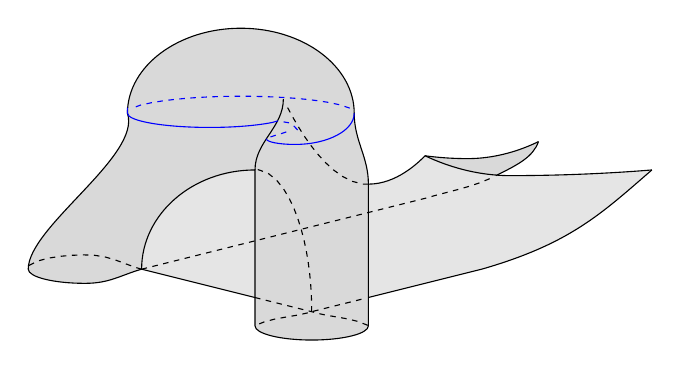
\begin{tikzpicture}[
			yscale=0.36, xscale=0.72,
			% This decoration will be used to make portions of curves into "bouckground curves". It allows us to dash a portion of the curve.
			decoration={border, 
				segment length = 4pt, 	% determines the distance between consecutive ticks.
				amplitude = 2pt, 		% determines the length of the ticks.
				angle = 0  				% determines the angle between the ticks and the line of the path. 
				}, 
			% Styles
			contour line/.style={thin, blue}
				]
				
			% Colors
			\colorlet{surfacecolor1}{black!15}
			\colorlet{surfacecolor2}{black!10}	
			
			% The graphic
			%\draw [step = 1cm, help lines] (-0.9,-0.9) grid (11.9, 10.9);
			
			% First we fill the surfaces with the background colors.
			% region 1
			\fill [color = surfacecolor1] (0, 2.5) .. controls (0, 4) and (2,6.5) .. (1.75,8)
				arc (180:0:2cm and 3cm)
				%.. controls (3, 9) and (3,10) .. (4,10)
				%.. controls (4.5,10) and (6,9.5) .. (6,8)
				to [out = 270, in = 90] (6, 5.5)
				-- (6,0.5)
				arc (360: 180: 1cm and 0.5cm)
				-- (4, 6)
				arc (90:180:2cm and 3.5cm)
				%.. controls (1, 2) and (1.5, 2) .. (1, 2)
				to [out = 210, in = 0] (1,2)
				arc (270: 180: 1cm and 0.5cm);
			
			% region 2
			\fill [color = surfacecolor1] (7, 6.5) parabola bend (8.5, 5.8) (8.25, 5.8) 
				to [out = 45, in = 260] (9, 7)
				parabola bend (7.75, 6.4) (7, 6.5);
			
			% region 3
			\fill [color = surfacecolor2] (4, 6) arc (90:180:2cm and 3.5cm)
				-- (4, 1.5) -- (4,6);
			
			% region 4
			\fill [color = surfacecolor2] (6, 5.5) parabola (7, 6.5) parabola bend (8.5, 5.8) (11, 6)
				to [out = 240, in = 30] (8, 2.5) -- (6, 1.5) -- (6, 5.5);
			
			
			% Now we draw the lines of the surface
			%first around region 1
			\draw (0, 2.5) .. controls (0, 4) and (2,6.5) .. (1.75,8)
				arc (180:0:2cm and 3cm)
				%.. controls (3, 9) and (3,10) .. (4,10)
				%.. controls (4.5,10) and (6,9.5) .. (6,8)
				to [out = 270, in = 90] (6, 5.5)
				-- (6,0.5)
				arc (360: 180: 1cm and 0.5cm)
				-- (4, 6)
				arc (90:180:2cm and 3.5cm)
				%.. controls (1, 2) and (1.5, 2) .. (1, 2)
				to [out = 210, in = 0] (1,2)
				arc (270: 180: 1cm and 0.5cm);
			
			% then the rest 
			\draw (2,2.5) -- (4,1.5) 
				decorate {-- (5,1) to [out = -30, in = 135] (6,0.5)
					  (4,0.5) to [out = 45, in = 210] (5,1) -- (6,1.5)} 
				-- (8, 2.5) to [out = 30, in = 240] (11, 6);
				% then off to cusp points
			\draw decorate { (5, 1) arc (0:90:1cm and 5cm)};
			\draw decorate {(2,2.5) -- (7,5) to [out = 30, in = 225] (8.25, 5.8)} to [out = 45, in = 260] (9, 7) ;
			\draw decorate {(2,2.5) to [out = 150, in = 0] (1,3) arc (90:180:1cm and 0.5cm)};
			% cusp
			\draw (4, 6) to [out = 90, in = 270] (4.5, 8.5);
			\draw (6, 5.5) decorate { parabola (4.5, 8.5)} (6, 5.5) parabola (7, 6.5)
				parabola bend (7.75, 6.4) (9, 7);
			\draw (7, 6.5) parabola bend (8.5, 5.8) (11, 6);
			
%		% now the contour lines
%		% the first contour line
%		\draw [contour line] (2.25, 10) arc (180:360:1.5cm and 0.5cm)
%			decorate {(2.25, 10) arc (180:0:1.5cm and 0.5cm)};
%		
%		
%		% the second contour line
		\draw [contour line] (1.75,8) arc (180:320:1.45cm and 0.5cm)
			decorate {to [out = 30,in = 135](4.65, 7.6) to [out = -45, in = 45] (4.2, 7.1) }
			arc (180:270:0.5cm and 0.2cm) to [out = 0, in = -90] (5.75,8)
		;
		\draw [contour line] decorate {(1.75,8) arc (180:0:2cm and 0.6cm)};
%		% the third contour line
%		\draw [contour line] 
%			decorate {(1.25, 5.75) arc (180:90: 1cm and 0.5cm) to [out = 0, in = 150] (3.5,5.75)}
%			 -- (4, 5.5) 
%			decorate {-- (4.5,5.25) to [out = -30, in = 135] (6,5)}
%			arc (360: 180: 1cm and 0.5cm)
%			decorate { to [out = 45, in = 210] (4.5,5.25)};
%		
%		\draw [contour line] 
%		 (1.25, 5.75) arc (180: 270: 1cm and 0.5cm) to [out = 0, in = 210] (3.25,5.75)
%		 	 to [out = 30, in = 150] (5.25, 6.15) to [out = -30,in = 30] (4.5, 5.25);
			
			%\draw (0,3) decorate {to (2,3)} -- (3,4);
				
		\end{tikzpicture}
		\end{center}	
	\caption{The Belt Bordism}
	\label{fig:belt_bordism}
\end{figure}




We prove that finite tensor categories are Radford objects in $\TC$, and the Serre automorphism of $\cC$ is $\cC$ as a $\cC$--$\cC$-bimodule category where the left action has been twisted by the right double dual functor.  The inverse of the Serre automorphism is the bimodule where the left action has been twisted by the left double dual.  Thus, the Radford equivalence relates the left double dual and the right double dual and recovers the generalization of Radford's theorem for finite tensor categories \cite{MR0407069, MR2097289} stating that the quadruple dual is canonically naturally isomorphic to conjugation by the distinguished invertible object $D$.  In addition, for fusion categories the distinguished object is trivial, and thus the quadruple dual for fusion categories is trivial.  

Altogether, an elegant, transparent topological fact, concerning the fundamental group of the space of $3$-framings, implies the a priori rather more opaque theorem that the quadruple dual on a fusion category is canonically trivializable. This makes rigorous the intuition (implicit in cite{MR2559711}, and stated explicitly in \cite{0901.3975}) that Radford's theorem is related to the belt trick.    Furthermore, this gives a generalization of Radford's theorem to any Radford object in any symmetric monoidal $3$-category (Prop.~\ref{prop-Cat_Radford}).

\NS{Should we say something about the O(3) action and the last subsection here?  I've collected some relevant commented out sections.}

%Being fully dualizable is a \emph{property} while being a homotopy fixed point is a choice of \emph{structure}.  Being fusion is a property (semisimple, finitely many simple objects, duals exist for each object), while being spherical is a structure (choice of natural isomorphism between the identity and the double dual).  

%The cobordism hypothesis also predicts the existence of an $O(3)$-action on the 3-groupoid of separable tensor categories, and in later papers in this series we will give a complete description of this action and of several important homotopy fixed point spaces in future work. In this work, we describe only a portion of this action. The underlying space of $SO(3)$ is $\RR \PP^3$. The inclusion $\RR \PP^2 \to \RR \PP^3 \simeq SO(3)$ induces an $A_\infty$-homomorphism $\Omega \Sigma (\RR \PP^2) \to SO(3)$ from the free $A_\infty$-group generated by the pointed space $\RR \PP^2$. We give a completely explicit and universal description of the $\Omega \Sigma (\RR \PP^2)$-action on the 3-groupoid of fully-dualizable objects of any symmetric monoidal 3-category, in particular on separable tensor categories. Moreover this explicit description allows us to show that this action extends to an action on the 3-groupoid of finite rigid tensor categories as well (a fact not deducible from the cobordism hypothesis itself).  
%\CSP{Is it too strong to say this fact is `not deducible' from the cobordism hypothesis? My feeling is it is okay, but would like other opinions.}




%Material possibly for intro to section: Traditionally topological field theories have been used as a tool to apply algebra to topology.  That is to say, a particular algebraic object yields a topological field theory which in turn gives topological invariants which can be used to prove results in topology.  However, the correspondence between algebra and topology can run the other way to give applications of topology to algebra.  A single topological calculation can be used to prove theorems in algebra by looking at the value of a bordism under a topological field theory.  In this section, we give one example of this correspondence, showing that Radford's theorem on the quadruple dual functor for finite tensor categories follows from the Dirac belt trick in topology.



\subsection*{Outline and results}
\addtocontents{toc}{\SkipTocEntry}

In Section \ref{sec:lft} we discuss local field theory.  Since $n$-framed bordisms are central to the cobordism hypothesis and therefore to the classification of local field theories, we begin by fixing a convenient notation for $n$-framings and we illustrate the notation with examples.  We then discuss the loop and belt bordisms and the corresponding notions of Serre and Radford equivalences.  Finally, we introduce the notion of a Radford object (which is stronger than $2$-dualizability, but weaker than $3$-dualizability) and give a direct short construction (not relying on the cobordism hypothesis) of a Radford equivalence attached to any Radford object.  We defer to the appendix several technical details concerning the model independence of the cobordism hypothesis and the constructability of the TFT attached to a fully dualizable object.

In Section \ref{sec:tc} we rapidly review the theory of finite tensor categories, bimodule categories, Deligne tensor product, exact bimodule categories, separable tensor categories, and fusion categories, and we prove several key structural lemmas.   In \S~\ref{sec:conventions} we fix some left/right conventions.  In \S~\ref{sec:tc-lincat} we collect some background material from the work of Etingof, Gelaki, Nikshych, and Ostrik (which is most comprehensively described in their lecture notes \cite{EGNO}) and from our papers \cite{BTP} and \cite{3TC}.  Experts in tensor categories can skip this subsection, referring back to it as needed, while readers who are not familiar with EGNO's theory are encouraged to read \cite{BTP} which is self-contained and contains proofs of all the background results needed for this paper.  In \S~\ref{sec:tc-exact} we rapidly review Etingof and Ostrik's theory of exact bimodule categories, and prove a new lemma on exactness of Deligne tensor products.  Section~\ref{sec:tc-bimodules} is new material consisting of several constructions of bimodule categories and some key lemmas for manipulating bimodule categories.  This section is used throughout the proofs of the main results.  Sections~\ref{sec:tc-separable} and \ref{sec:tc-fusion} introduce spearable tensor categories and consists mostly of new material some of which extends results of M\"uger, Etingof--Niksych--Ostrik, and Brugui\`res--Virelizier.  These subsections are technical and aimed at experts.  The reader interested only in characteristic zero can skip these sections.

The heart of the paper is Section \ref{sec:dualizability} where we prove the following main results.

\CSP{Change the numbering of these theorems to match the correct numbering in the paper.}
\CD{I vote for dealing with the numbering slightly differently --- I'll implement it and you can see if you like it --- if not, we can then do what you propose.}

\begin{maintheorem} \label{thm1}
Separable tensor categories are fully dualizable.
\end{maintheorem}

\nid Note that separability is a technical condition which is automatic over a field of characteristic $0$, and is equivalent nonzero global dimension for fusion categories over an algebraically closed field.

A key application of this theorem is the construction of a plethora of local field theories:
\begin{maincor} \label{cor2}
For any separable tensor category there is a local topological quantum field theory whose value on a point is that tensor category.
\end{maincor}

\nid Strictly speaking, this TFT is not directly comparable to Turaev--Viro theories, since it is $3$-framed rather than oriented, and it does not depend on either the choice or existence of a spherical structure.  Nonetheless, it should be thought of as a generalization of Turaev--Viro.

We also have a converse to the main theorem.

\begin{maintheorem} \label{thm3}
Fully dualizable finite tensor categories are separable.
\end{maintheorem}

For technical reasons we restrict our attention throughout to finite tensor categories throughout this paper, because we have only given a rigorous definition of the $3$-category of finite tensor categories.  In particular, the relative Deligne tensor product is not easy to define in more generality.  Nonetheless, it is natural to wonder whether finiteness or even rigidity (which is part of the definition of tensor category) are necessary for dualizability.  Since rigidity is not preserved by Morita equivalence (as pointed out to us by Dan Freed), there are finite monoidal categories which are fully dualizable but not rigid.  Indeed, semisimplicity and finiteness are also not Morita invariant notions.  We do not know a simple characterization of all fully dualizable monoidal categories (indeed we do not know in what generality it even makes sense to ask this question).

We also establish that there are field theories associated to finite tensor categories that are not necessarily separable:

\begin{maintheorem} \label{thm4}
Finite tensor categories are $2$-dualizable.
\end{maintheorem}

An $n$-dimensional topological field theory which takes values in an $(n+1)$-category is in a sense `categorified'.  For example, in dimension two such a field theory would sends surfaces to vector spaces rather than numbers.  As usual, the categorified structure has extra richness, in this case the vector spaces would then inherit actions of mapping class groups. The prototypical example of a categorified TFT is the concept of a {\em modular functor}.  For another example of a categorified $2$-dimensional TFT see \cite{0904.1247}.

\begin{maincor} \label{cor5}
Any finite tensor category gives a $2$-framed local $2$-dimensional TFT which is categorified in the above sense. 
\end{maincor}

We give a concrete application of these results to Radford's theorem.

\begin{maintheorem} \label{thm6}
The Serre automorphism of a finite tensor category $\cC$ is the bimodule associated to the double dual functor ${}^{**}(-): \cC \ra \cC$.  %!%Once we adjust all the conventions, this will be the left double dual.
\end{maintheorem}

In $3$-dimensions, the Serre automorphism is necessarily order $2$ (since $\pi_1(SO(3)) \cong \mathbb{Z}/2$). This theorem therefore provides a simple topological proof of the following generalization Radford's theorem \cite{MR0407069} to fusion categories (originally due to Etingof, Nikshych, and Ostrik \cite{MR2183279}).
\begin{maincor} \label{cor7}
The quadruple dual functor ${}^{****}(-): \cC \ra \cC$ on a fusion category is naturally isomorphic to the identity functor.
\end{maincor}

We then address how this result generalizes to finite tensor categories.  Although $2$-dualizability is not enough to prove Radford's theorem  (we need a $3$-framed theory, not a $2$-framed theory), finite tensor categories have certain additional adjoints for $2$-morphisms which makes them Radford objects.  Thus our ``belt trick" approach to the quadruple dual generalizes to Radford objects, and thus gives a proof of the generalization of Radford' theorem to finite rigid tensor categories (again due to Etingof, Nikshych, and Ostrik \cite{MR2097289}).  This argument does not depend on the proof of the cobordism hypothesis, as it is much easier to construct the value of one particular bordism than it is to construct a whole TFT.

\begin{maincor} \label{cor8}
The quadruple dual functor ${}^{****}(-): \cC \ra \cC$ on a finite tensor category is naturally isomorphic to conjugation by the distinguished invertible object $D$.
\end{maincor}

We conclude with a brief discussion about $\Omega \Sigma \RP^2$ fixed points and their relationship to the Serre and Radford equivalences and to pivotal and spherical structures.  Surprisingly, it turns out that the right generalization from the point of view of topology of spherical structures to non-semisimple categories differs from the usual notion of spherical.  In later papers we will consider the full $SO(3)$.

\CD{Somewhere in intro, explain that we identify the $\Omega \Sigma \RP^2$ action and will do the $SO(3)$ action in sequels.}

\subsection*{Relationship to other work}
\addtocontents{toc}{\SkipTocEntry}

The history of local field theories is somewhat complicated, as the language took some time to catch up to the results.  Some versions of a $123$ extended field theory go back quite early in the literature, where the $12$ part of the theory is called a ``modular functor" \cite{Segal, MR1002038, MR1159969,MR1797619}.  In particular, Turaev's book \cite{MR1292673} can be thought of as roughly giving a $123$ extended field theory attached to a modular tensor category.  However, the assumption that the category be modular (or even braided) is too strong.  Kerler-Lyubashenko \cite{MR1862634} construct a somewhat unusual partial $123$ field theory associated to not-necessarily semisimple modular tensor categories.   A rigorous $123$ version of Turaev--Viro in fully modern language is given in the work of Balsam--Kirillov \cite{1004.1533}.  Finally, Kevin Walker and Scott Morrison's work \cite{kw:tqft, 1009.5025} gives a local version of the Turaev--Viro TFT in a different language (disc-like $n$-categories) which is of a more topological flavor than other algebraic notions of $n$-category.
\NS{I can't think of any more references to put in here, but maybe there should be.}

All of the above work on TFTs from fusion categories assumes sphericality in an essential way.  The history of framed field theories is a bit different.  Here the main precursors are the theory of spin TFTs \cite{MR1117149, MR1171303, MR1387228, MR1880321}, and Kuperberg's work on $3$-manifold invariants coming from nonsemisimple Hopf algebras \cite{MR1394749}.

Most previous examples of fully dualizable objects are in dimension $2$.  Schommer-Pries's thesis proves $2$-dualizability of separable algebras \cite{schommer-pries-thesis}.    Ben-Zvi--Nadler \cite{0904.1247} prove $2$-dualizabilty for certain monoidal categories, but in the derived category setting instead of the abelian setting of this paper.   Two other programs closely related to ours are Bartels--Douglas--Henriques \cite{0912.5307} and work in progress of Freed--Teleman who look at different versions of local Witten--Reshetikhin--Turaev field theories \cite{MR990772, MR1091619} through the lens of the cobordism hypothesis. \NS{We should ask Freed--Teleman if they have a title.}

The original version of Radford's theorem \cite{MR0407069} is an explicit formula for the fourth power of the antipode in a finite-dimensional Hopf algebra.  This was generalized to the context of fusion categories, and then to finite rigid tensor categories by Etingof--Nikshych--Ostrik \cite{MR2183279,MR2097289}.  The first indication that Radford's formula is related to topology came in Kuperberg's proof of Radford's theorem for Hopf algebras (and indeed Hopf algebra objects in symmetric tensor categories) \cite{MR1394749}.  Next Hagge--Hong \cite{MR2559711} gave a skein theoretical proof of Radford's theorem for fusion categories.  As pointed out by Bartlett \cite{0901.3975} the Hagge--Hong proof is reminiscent of the belt trick.

\subsection*{Future directions}
\addtocontents{toc}{\SkipTocEntry}

There are several directions in which we hope to take this project. We briefly summarize them here.

The belt trick corresponds to the action of $\pi_1(SO(3)) = \mathbb{Z}/2\mathbb{Z}$ on the space of fusion categories.  But this is only a small part of the information of an $SO(3)$ action.  In later papers we will explicitly describe the full action of $SO(3)$ and understand homotopy fixed points for the action of $SO(3)$ and of several related groups.  By the cobordism hypothesis, homotopy fixed points for $SO(3)$ correspond to oriented field theories.  This point of view clarifies many notions in the theory of fusion categories, for example we expect that spherical fusion categories are a certain kind of $SO(3)$ fixed point, while pivotal fusion categories are a certain kind of $SO(2)$ fixed point.  We expect to give topological proofs of several ``anomaly vanishing" results generalizing a result of M\"uger \cite{MR1966525} to the non-spherical setting.

As we note at several points in the paper, finite tensor categories give a field theory which is defined on certain kinds of $3$-dimensional bordisms, but not all $3$-dimensional bordisms---we call these field theories non-compact, in the spirit of Costello's work \cite{MR2298823} in dimension $2$, and Lurie's generalizations \cite[\S 4.2]{lurie-ch}.  In order to construct a non-compact $3$-dimensional theory we need a non-compact analogue of the cobordism hypothesis in dimension $3$.  We defer detailed investigation of such matters to future work.

We do not prove in this paper that our $3$-manifold invariants actually agree with Turaev--Viro in the spherical case.  Indeed, to even make such a statement rigorous we would need to prove that spherical structures give $SO(3)$ fixed point structures, which we do not do in this paper.  Though it is worth noting that by the uniqueness part of the cobordism hypothesis, the construction of a fully extended version of Turaev--Viro via other techniques would automatically show that our construction also gives Turaev--Viro.  We hope in the future to give a more direct proof that our $3$-manifold invariants can be computed by state-sums.  Similarly we hope to give a direct calculation showing that our TFT for a spherical fusion category $\cC$ agrees with the Reshetikhin--Turaev TFT for the Dringel'd center $\cZ(\cC)$.  (By \cite{1006.3501} Turaev--Viro for $\cC$ and Reshetikhin--Turaev for $\cZ(\cC)$ agree, but it may be possible to get directly from our construction to Reshetikhin--Turaev without going through state sums.)

Finally, the assumptions that we use to get $2$-dualizability (finite and rigid) are too strong, and we hope to generalize that result to other monoidal categories.  This depends on constructing a more general version of the Deligne tensor product.

\subsection*{Higher categories} 
\addtocontents{toc}{\SkipTocEntry}

In this paper, we work with symmetric monoidal 3-categories in a model free way, rather than fixing one of many options for axiomatizing 3-categories.  This may make certain readers nervous, and to those readers we offer two assurances.  First, in \cite{3TC} we show that everything in this paper can be made precise in a particular choice of model.  Second, every major theorem in this paper is actually only a statement about 2-categories (either by restricting to a Hom 2-category between objects, or by identifying all isomorphic 2-morphisms), and the theory of 2-categories does not suffer from any of the theoretical complications of higher categories.  It is only the corollaries which relate the algebraic theorems to local TFTs which depend (via the cobordism hypothesis) on having a robust theory of categories in dimensions above 2.  More specifically, Theorems \ref{thm1}, \ref{thm3}, \ref{thm4}, and \ref{thm6}, and Corollaries \ref{cor7} and \ref{cor8} depend neither
on the theory of higher categories nor on the cobordism hypothesis;
Corollary \ref{cor5} depends on the theory of $(\infty,2)$-categories and on the
cobordism hypothesis in dimension 2; and Corollary \ref{cor2} depends on the theory
of $(\infty,3)$-categories and on the cobordism hypothesis in dimension
3.  \CD{Recheck the list of `things in the paper that use CH'}

\subsection*{Acknowledgments}
\addtocontents{toc}{\SkipTocEntry}

We would like to thank Ben Balsam, Dan Freed, Mike Hopkins, Alexander Kirillov Jr., Scott Morrison, Stephan Stolz, Constantin Teleman, Peter Teichner, Dylan Thurston, and Kevin Walker for helpful conversations.   For the first six months of this project we collaborated using Google Wave, and we would like to thank the Google Wave team for their work.  \NS{Anyone else want to add people to the list of non-special thanks?  I feel like one should err on the side of mentioning too many people. CD: I can't think of anyone else.}

We are especially grateful to Victor Ostrik for a key suggestion which lead to the arguments in Section \ref{sec:tc-fusion}.
NS would especially like to thank Pavel Etingof for several long and fruitful conversations.  CD would like to especially thank Andr\'e Henriques for general enlightenment and specific ideas regarding the 3-category of tensor categories and 3-dimensional local field theory.

\CD{In intro, mention that in effect we provide a generalization of Radford's theorem to any Radford object in any symmetric monoidal 3-category}

\section{Local field theory in dimension three} \label{sec:lft}

\CDh{\S 2.0 $\checkmark$}


The cobordism hypothesis \cite{MR1355899, lurie-ch} classifies local field theories in terms of sufficiently dualizable objects of target higher categories.  Recall that an object $x$ of a symmetric monoidal $(\infty,3)$-category is called ``1-dualizable" if there is a dual object $\overline{x}$, with the duality between $x$ and $\overline{x}$ witnessed by evaluation and coevaluation maps $ev: x \otimes \overline{x} \ra 1$ and $coev: 1 \ra \overline{x} \otimes x$.  (Note well that the zigzag equations relating $ev$ and $coev$ are only required to hold up to equivalence, and there is no coherence condition on those equivalences.)  The object is called ``2-dualizable" if moreover the evaluation map is part of an infinite chain of adjunctions 
$$\cdots \dashv ev^{LL} \dashv ev^L \dashv ev \dashv ev^R \dashv ev^{RR} \dashv \cdots$$
and similarly the coevaluation map is part of an infinite chain of adjunctions 
$$\cdots \dashv coev^{LL} \dashv coev^L \dashv coev \dashv coev^R \dashv coev^{RR} \dashv \cdots.$$  
(Again, note that for each of these adjunctions, the zigzag equations are only required to hold up to isomorphism, and there are no coherence conditions on those isomorphisms.)
The object is called ``3-dualizable", also known as ``fully dualizable", if, moreover, for every adjunction $(F \dashv G, u_{F,G}, v_{F,G})$ in each of the two aforementioned infinite chains, it happens that the unit $u_{F,G}$ is part of an infinite chain of adjunctions 
$$\cdots \dashv u_{F,G}^{LL} \dashv u_{F,G}^L \dashv u_{F,G} \dashv u_{F,G}^R \dashv u_{F,G}^{RR} \dashv \cdots$$ 
and similarly the counit $v_{F,G}$ is part of an infinite chain of adjunctions 
$$\cdots \dashv v_{F,G}^{LL} \dashv v_{F,G}^L \dashv v_{F,G} \dashv v_{F,G}^R \dashv v_{F,G}^{RR} \dashv \cdots.$$  These definitions suffice to make sense of our main theorem, that every separable tensor category is fully dualizable.  
%!% CD to discuss with CSP this definition: confirm that he agrees that it is obviously equivalent, because any equivalence can be promoted to an adjoint equivalence, and those adjoint equivalences can be used to transport the dualization structure to the other object.  In particular, Jacob's use of "essential image" was a red-herring, arising from the way Jacob decided to define the f.d. subcategory as anything satisfying the universal property.

It will be more convenient for us to use an alternative, equivalent formulation of dualizability focusing on ``$k$-dualizable $3$-categories" rather than ``$k$-dualizable objects."  A symmetric monoidal $3$-category $\cC$ is called ``$1$-dualizable" if every object has a dual---as before, here `dual' means dual in the symmetric monoidal $1$-category of objects of $\cC$ and equivalence classes of morphisms of $\cC$.  The symmetric monoidal $3$-category $\cC$ is called ``$2$-dualizable" if it is 1-dualizable and moreover every $1$-morphism has a left and a right adjoint---as before, here `adjoint' means adjoint in the $2$-category of objects, morphisms, and isomorphism classes of 2-morphisms of $\cC$.  The symmetric monoidal $3$-category $\cC$ is called ``$3$-dualizable", also called ``fully dualizable", if it is $1$-dualizable and $2$-dualizable and if every $2$-morphism of $\cC$ has a left and a right adjoint.  An object of a symmetric monoidal $3$-category is ``fully dualizable" if it is in some fully dualizable subcategory of $\cC$.  %!% CD to again confirm that CSP agrees with this last sentence.
(There are corresponding notions of fully-dualizable objects of an $n$-category, for any $n$.)

Equipped with the notion of full dualizability, we can state the cobordism hypothesis classification of local field theories: \vspace{7pt}

\setlength{\leftskip}{.75cm}

\nid {\bfseries Cobordism hypothesis:} \emph{$n$-dimensional local framed topological field theories with target a symmetric monoidal $(\infty,n)$-category $\cC$ are in one-to-one correspondence with the fully dualizable objects of $\cC$; in fact, the space of such field theories is homotopy equivalent to the space of fully dualizable objects of $\cC$.} \vspace{7pt}

\setlength{\leftskip}{0cm}

\nid By definition, an $n$-dimensional local framed topological field theory is a symmetric monoidal functor out of the $(\infty,n)$-category $\FrBord_n$ of $n$-framed bordisms.  In the next section we describe the notion of $n$-framing in question.  We refer the reader to Appendix~A for a more detailed and precise review of the notion of full dualizability and statement of the cobordism hypothesis.  

\subsection{$n$-framed bordisms} \label{sec:notation}
\CDh{\S 2.1 $\checkmark$}


In the first instance, the cobordism hypothesis classifies field theories whose source is a bordism category of $n$-framed manifolds.  In this section, we describe a convenient notation for describing $n$-framed manifolds using normally framed immersions, and explain how this notation behaves on boundaries and corners and thereby produces bordism categories.  We conclude with various low dimensional examples, many of which will also be essential in our later dualizability calculations.

\subsubsection{$n$-framings from normally framed immersions}

An $n$-framed $k$-manifold $(M,\tau)$ is, by definition, a $k$-manifold $M$ equipped with a trivialization $\tau$ of $TM \oplus \RR^{n-k}$, the $(n-k)$-fold stabilization of the tangent bundle of $M$.  A convenient way to present an $n$-framing on a $k$-manifold $M$ is to give an immersion $\iota: M \looparrowright \RR^n$ together with a framing, that is trivialization, $\phi$ of the normal bundle $\nu(\iota)$ of the immersion.  The normally framed immersion $(\iota, \phi)$ provides an $n$-framing of $M$ by the composite
\[
TM \oplus \RR^{n-k} \cong TM \oplus \nu(\iota) \cong \RR^n.
\]
Here the second isomorphism is provided by the standard, ``blackboard" framing of the sum of the tangent bundle and normal bundle of $M$.

Throughout this paper, except in one noted exception, we will draw $n$-framed manifolds using this normally framed immersion notation; in particular we depict the immersion and the normal framing and leave completely implicit the induced $n$-framing.  When the immersion is codimension-1, we will usually specify the normal framing by a unidirectional gray corona on the immersed manifold.

\begin{example} \label{eg:frcircles}
The following infinite list evidently includes, up to homotopy, all normally framed immersed circles in $\RR^2$:
\[\cdots\quad
\cb{
\begin{tikzpicture}
{ [xshift=-3cm]
\draw[linestyle,fuzzleft]
(.5,0) to [out=-90, in=25] (.3,-.3)
	to [looseness=1.6, out=-155, in=225] (.15,-.15)
	to [looseness=1.6, out=45, in=65] (.3,-.3)
	to [out=245, in=-65] (-.3,-.3)
	to [looseness=1.6, out=115, in=135] (-.15,-.15)
	to [looseness=1.6, out=-45, in=-25] (-.3,-.3)
	to [out=155, in=-90] (-.5,0)
	.. controls (-.5,.66) and (.5,.66) .. (.5,0);	
}
{ [xshift=-1.5cm]
\draw[linestyle,fuzzleft]
(.5,0) to [out=-90, in=-20] (0,-.4)
	to [looseness=1.6, out=160, in=180] (0,-.1)
	to [looseness=1.6, out=0, in=20] (0,-.4)
	to [out=-160, in=-90] (-.5,0)
	.. controls (-.5,.66) and (.5,.66) .. (.5,0);
}
{ [xshift=0cm]
\draw[linestyle,fuzzleft]
(.5,0) .. controls (.5,-.66) and (-.5,-.66) .. (-.5,0)
	.. controls (-.5,.66) and (.5,.66) .. (.5,0);
}
{ [xshift=1.5cm]
\draw[linestyle,fuzzleft,looseness=2]
(0,.5) to [out=0, in=10] (0,0)
	to [out=-170, in=180] (0,-.5)
	to [out=0, in=-10] (0,0)
	to [out=170, in=180] (0,.5);
}
{ [xshift=3cm]
\draw[linestyle,fuzzright]
(.5,0) .. controls (.5,-.66) and (-.5,-.66) .. (-.5,0)
	.. controls (-.5,.66) and (.5,.66) .. (.5,0);
}
{ [xshift=4.5cm]
\draw[linestyle,fuzzright]
(.5,0) to [out=-90, in=-20] (0,-.4)
	to [looseness=1.6, out=160, in=180] (0,-.1)
	to [looseness=1.6, out=0, in=20] (0,-.4)
	to [out=-160, in=-90] (-.5,0)
	.. controls (-.5,.66) and (.5,.66) .. (.5,0);
}
{ [xshift=6cm]
\draw[linestyle,fuzzright]
(.5,0) to [out=-90, in=25] (.3,-.3)
	to [looseness=1.6, out=-155, in=225] (.15,-.15)
	to [looseness=1.6, out=45, in=65] (.3,-.3)
	to [out=245, in=-65] (-.3,-.3)
	to [looseness=1.6, out=115, in=135] (-.15,-.15)
	to [looseness=1.6, out=-45, in=-25] (-.3,-.3)
	to [out=155, in=-90] (-.5,0)
	.. controls (-.5,.66) and (.5,.66) .. (.5,0);	
}
\end{tikzpicture}
}
\quad \cdots
\]
As described above, each such immersion specifies a $2$-framed circle, and in fact all $2$-framed circles are so specified.  Suppose we have a $2$-framing $\tau: TM \oplus \RR \xra{\cong} \RR^2$ on a closed connected 1-manifold $M$.  Let $\jmath$ denote the orientation of $M$ such that for any point $p \in M$, the pair $(\tau(\jmath,0),\tau(0,1))$ is a positive frame of $\RR^2$.  This orientation provides another $2$-framing of $M$, namely $\sigma: TM \oplus \RR \xra{\jmath \oplus \id} \RR^2$.  The ratio $\sigma/\tau$ is a map $M \ra SO(2)$.  Because $M$ is oriented, by $\jmath$, the set of homotopy classes of maps $M \ra SO(2)$ is canonically identified with the integers.  We therefore have a $\ZZ$-valued invariant of such $2$-framed 1-manifolds, and in fact this procedure produces an isomorphism from the $2$-framed diffeomorphism classes of $2$-framed closed connected 1-manifolds to the integers---the above picture provides a representative from each diffeomorphism class.
\end{example}

\begin{remark}
Not every $n$-framed $n$-manifold can be specified using the immersion notation.  For example, the circle has a (unique up to diffeomorphism) $1$-framing, but it cannot be immersed in $\RR^1$.  The Hirsch-Smale immersion theorem \cite{MR0119214, MR0105117} ensures, though, that every $n$-framing of an $(n-k)$-manifold can be realized by a normally framed immersion, provided either $k>0$ or each component of the manifold is not closed.
\end{remark} %!% CD not checked

An $m$-framed $k$-manifold $(M,\tau)$ can be stabilized to an $n$-framed manifold $(M,\tau \oplus \id_{\RR^{n-k}})$.  A normally framed immersion $(\iota: M \looparrowright \RR^m, \phi : \nu(\iota) \simeq \RR^{m-k})$ can similarly be stabilized to the normally framed immersion $(\inc_{\RR^m \ra \RR^n} \circ \iota, \phi \oplus \RR^{n-m})$.  The association of an $m$-framed manifold to a normally framed immersion is evidently compatible with these stabilization procedures.

\begin{example}
Though the 1-framing on the circle cannot be represented by a normally framed immersion, its stabilization to a 2-framing can: it is represented by the figure 8 immersion in Example~\ref{eg:frcircles}.
\end{example}


\subsubsection{$n$-framings with boundary and corners}

The procedure described above for associating an $n$-framed manifold to a normally framed immersion works as stated also for manifolds with boundary or manifolds with corners.  Moreover, when the immersed manifold is a bordism, we can fix conventions for how a normal framing (therefore $n$-framing) on the bulk induces a normal framing (therefore $n$-framing) on the source and target boundary.  For a bordism $M$ with boundary but without corners, each boundary component is labelled ``in" or ``out" according to whether it is part of the source or target of the bordism.  Suppose $(\iota, \phi)$ is a normally framed immersion of $M$.  An incoming boundary component $N \subset (\partial M)_{\textrm{in}}$ inherits the structure of a normally framed immersion: the immersion is simply the restriction of the immersion of $M$, and the framing is $(l,s) \subset \nu(N,\RR^n)$, where $l$ is a section of the normal bundle of $N$ pointing into the bulk manifold $M$, and $s \subset \nu(M,\RR^n)$ is the given normal frame of $M$.  Similarly an outgoing boundary component inherits the normal framing $(-l,s)$, that is the first normal frame vector points out of the bulk manifold.  Given a higher bordism (that is a manifold $M$ with cuspidal corners representing a higher morphism in a bordism $n$-category), equipped with a normally framed immersion, the incoming and outgoing boundaries (which are now codimension-0 submanifolds of the boundary of $M$) inherit normal framings exactly as described for ordinary bordisms.  Furthermore, the boundaries of these boundaries inherit normal framings by the same procedure.  Iterating this process provides consistently defined normal framings to every corner of the higher bordism $M$.  We provide various examples of such manifolds and the associated induced framings in the next section.

In drawing $n$-framed manifolds with boundary and corners, we need to specify not only the immersion and the normal framing, but also which parts of the boundary are incoming and which outgoing.  Outgoing pieces of the boundary will be indicated by small arrows pointing out of the bulk of the manifold; incoming pieces of the boundary will be undecorated---implicitly the arrows would point into the bulk.  When the immersion is codimension zero, the outgoing boundary arrows may be replaced by a gray corona, which serves to directly record the induced normal framing of those parts of the boundary.  At corners, a combination of these indications will be used; for instance, an arrow together with a corona on a codimension-2 corner indicates respectively the first and second vectors of the induced framing on the corner.

\begin{remark}
If $M$ is an $n$-manifold with boundary immersed in $\RR^n$, the corona indicates which boundaries are outgoing, while if $M$ is an $(n-1)$-manifold with boundary immersed in $\RR^n$, the corona indicates the trivialization of the normal bundle.  These two usages are compatible: the induced trivialization of the normal bundle of the outgoing boundary is indeed the outward trivialization, therefore indicated by an outward corona.  The trivialization of the normal bundle of an incoming boundary is the inward trivialization, therefore would be indicated by a corona pointing into the bulk manifold; this type of corona is covered by the bulk and so cannot be seen.
\end{remark}


\subsubsection{Low-dimensional examples of $n$-framed bordisms}

\begin{example} \label{eg-framenot0}
The following four pictures specify respectively a $0$-framed, a $1$-framed, and two $2$-framed 0-manifolds:
\[
\begin{tikzpicture}
\filldraw (0,0) circle (\pointrad);
\filldraw (1,0) circle (\pointrad); 
\begin{pgfonlayer}{background}
\draw[->,outstyle] (1,0) -- +(-\arrowlength,0);
\end{pgfonlayer}
\filldraw (2,0) circle (\pointrad);
\begin{pgfonlayer}{background}
\draw[->,outstyle] (2,0) -- +(45:\arrowlength) node[anchor=south,inner sep=2pt] {\tiny 1};
\draw[->,outstyle] (2,0) -- +(135:\arrowlength) node[anchor=south,inner sep=2pt] {\tiny 2};
\end{pgfonlayer}
\filldraw (3,0) circle (\pointrad); 
\begin{pgfonlayer}{background}
\draw[->,outstyle] (3,0) -- +(45:\arrowlength) node[anchor=south,inner sep=2pt] {\tiny 2};
\draw[->,outstyle] (3,0) -- +(135:\arrowlength) node[anchor=south,inner sep=2pt] {\tiny 1};
\end{pgfonlayer}
\end{tikzpicture}
\]
\end{example}

\begin{example}
Here is a picture of a $1$-framed $1$-manifold bordism from a 1-framed point to a 1-framed point:
\[
\begin{tikzpicture}
\draw[linestyle] (0,0) -- (1.5,0);
\begin{pgfonlayer}{background}
\draw[->,outstyle] (0,0) -- +(180:\arrowlength);
\end{pgfonlayer}
\path
    ([shift={(-5\pgflinewidth,-5\pgflinewidth)}]current bounding box.south west)
    ([shift={( 5\pgflinewidth, 5\pgflinewidth)}]current bounding box.north east);
\end{tikzpicture}
\]
\nid The right point is incoming and the left point is outgoing.  Both boundary points inherit framings isomorphic to the framing of the second picture in Example~\ref{eg-framenot0}.

Next we have a picture of a $2$-framed $1$-manifold bordism from two 2-framed points to the empty set:
\[
\begin{tikzpicture}
\draw[linestyle,fuzzleft] 
(0,0) .. controls (1.1,1.1) and (1.25,.65) .. (1.25,.5)
	.. controls (1.25,.25) and (.875,.25) .. (.875,.5)
	.. controls (.875,.9) and (1.875,.9) .. (1.875,.5)
	.. controls (1.875,.25) and (1.5,.25) .. (1.5,.5)
	.. controls (1.5,.65) and (1.65,1.1) .. (2.75,0);
\end{tikzpicture}
\]
Both boundary points are incoming, and the induced framings on these points are, left to right respectively, the last two points pictured in Example~\ref{eg-framenot0}.  Note that corona in this example specifies the trivialization of the normal bundle.
\end{example}

\begin{example} \label{ex:disk_bordism_immersed}
The following is a picture of a $2$-framed $2$-manifold bordism from the empty set to a 2-framed circle:
\[
u_1 := \cb{
\begin{tikzpicture}
\filldraw[linestyle,fuzzright,fill=\fillcolor] (0,0) circle (.5);
\end{tikzpicture}
}
\quad
:
\quad
\cb{$\emptyset$}
\quad \ra \quad
\cb{
\begin{tikzpicture}
\draw[linestyle,fuzzleft]
(.5,0) .. controls (.5,-.66) and (-.5,-.66) .. (-.5,0)
	.. controls (-.5,.66) and (.5,.66) .. (.5,0);
\end{tikzpicture}
}
\]
Note that in the picture of the 2-manifold $u_1$, the corona indicates that the boundary is outgoing.  That boundary is the circle with the outward trivialization of its normal bundle, and so the two uses of the corona are consistent, as mentioned previously.
\end{example}

\begin{example} \label{ex:saddle_bordism_immersed}
We now provide an example of a 2-framed 2-manifold with cuspidal corners, representing a 2-morphism in the 2-category of 2-framed 0-, 1-, and 2-manifolds:
\[
v_1 := \cb{
\begin{tikzpicture}
\filldraw[linestyle,fill=\fillcolor] 
	(0,0) .. controls (.25,.25) and (.75,.25) .. (1,0)
		.. controls (.75,.25) and (.75,.75) .. (1,1)
		.. controls (.75,.75) and (.25,.75) .. (0,1)
		.. controls (.25,.75) and (.25,.25) .. (0,0);
\draw[linestyle,fuzzright]
	(0,0) .. controls (.25,.25) and (.75,.25) .. (1,0);
\draw[linestyle,fuzzleft]
	(0,1) .. controls (.25,.75) and (.75,.75) .. (1,1);
\begin{pgfonlayer}{background}
	\draw[->,outstyle] (1,1) -- +(45:\arrowlength);
	\draw[->,outstyle] (1,0) -- +(-45:\arrowlength);
\end{pgfonlayer}
\end{tikzpicture}
}
\quad
: 
\quad
\cb{
\begin{tikzpicture}
\draw[linestyle,fuzzright]
	(0,0) .. controls (.25,.25) and (.25,.75) .. (0,1);
\draw[linestyle,fuzzleft]
	(1,0) .. controls (.75,.25) and (.75,.75) .. (1,1);
\begin{pgfonlayer}{background}
	\draw[->,outstyle] (1,1) -- +(45:\arrowlength);
	\draw[->,outstyle] (1,0) -- +(-45:\arrowlength);
\end{pgfonlayer}
\end{tikzpicture}
}
\quad
\ra
\quad
\cb{
\begin{tikzpicture}
\draw[linestyle,fuzzright]
	(0,0) .. controls (.25,.25) and (.75,.25) .. (1,0);
\draw[linestyle,fuzzleft]
	(0,1) .. controls (.25,.75) and (.75,.75) .. (1,1);
\begin{pgfonlayer}{background}
	\draw[->,outstyle] (1,1) -- +(45:\arrowlength);
	\draw[->,outstyle] (1,0) -- +(-45:\arrowlength);
\end{pgfonlayer}
\end{tikzpicture}
}
\]
The source and target of the bordism are the pairs of intervals indicated.  Notice that the source of the source (a pair of 2-framed points) is indeed the source of the target, and similarly the target of the source is the target of the target.
\end{example}

\begin{example} \label{eg:radford}
Figure~\ref{fig:belt_bordism} in the introduction can be equipped with a normal framing (pointing out of the page on the more lightly shaded regions of the bordism), with a corona indicating the outgoing boundary (pointing downward on the lower boundary), and with arrows indicating the outgoing boundary of the boundary (pointing rightward at the two cusps), so that it represents a 3-framed 2-manifold bordism.  The source of this bordism is the stabilization of the 2-framed 1-manifold,
\[
\cb{
\begin{tikzpicture}
	\draw[linestyle,fuzzright] (4,7) to [looseness=1.6,out = 180, in = 180] (4,6);
	\begin{pgfonlayer}{background}
		\draw[->,outstyle] (4,7) -- +(0:\arrowlength);
		\draw[->,outstyle] (4,6) -- +(0:\arrowlength);
	\end{pgfonlayer}
\end{tikzpicture}
}
\]
and target of the bordism is the stabilization of the 2-framed 1-manifold
\[
\cb{
\begin{tikzpicture}
	\draw[linestyle,fuzzright] (4, -0.5) -- (1.75, -0.5)
%	\draw[linestyle,fuzzright] (2,-.5) arc (270:0:\minirad);
%	\draw[linestyle,fuzzright] (2+\minirad,-.5+\minirad) -- (2,-1.75);
%		to [rounded corners=1cm] +(-.25,0)
%		to [rounded corners=1cm] +(0,.25)
%		to [rounded corners=1cm] +(.25,0)
%		to [rounded corners=1cm] +(0,-.25)
%
%		to [looseness=1.4, out=180,in=225] +(-.25,.25)
%		to [looseness=1.4, out=45,in=90] +(.25,-.25)
%
		to [looseness=2,out = 180, in = 90] (2, -0.25)
%	\draw[linestyle,fuzzright]
		-- (2, -1.75)
		to [looseness=2,out = 270, in = 180] (1.75,-1.5)
		-- (4, -1.5);
	\begin{pgfonlayer}{background}
		\draw[->,outstyle] (4,-0.5) -- +(0:\arrowlength);
		\draw[->,outstyle] (4,-1.5) -- +(0:\arrowlength);
	\end{pgfonlayer}
\end{tikzpicture}
%\begin{tikzpicture}
%\draw[linestyle,fuzzright] 
%(.7,0) to [out=180, in=-20] (0,.1)
%	to [looseness=1.6, out=160, in=180] (0,.4)
%	to [looseness=1.6, out=0, in=20] (0,.1)
%	to [looseness=1, out=-160, in=-20] (-.8,.1)
%	to [looseness=1.6, out=160, in=180] (-.8,.4)
%	to [looseness=1.6, out=0, in=20] (-.8,.1)
%	to [out=-160, in=0] (-1.5,0);
%\begin{pgfonlayer}{background}
%	\draw[->,outstyle] (.7,0) -- +(0:\arrowlength);
%\end{pgfonlayer}
%\end{tikzpicture}
}
\]
\end{example}


\subsection{Duality in the 2-framed bordism category}\label{sec:framed-duality}
\CDh{\S 2.2 $\checkmark$}


The 2-framed bordism 2-category is (like all typical bordism categories) fully dualizable.  In this section we explicitly illustrate all the duals and adjunctions in this 2-category.

There are two 2-framed diffeomorphism classes of 2-framed points.  We focus on the following representatives of these classes:
\begin{center}
\raisebox{2.2mm}{
\begin{tikzpicture}
	\filldraw (0,0) circle (\pointrad); 
	\begin{pgfonlayer}{background}
	\draw[->,outstyle] (0,0) -- +(90:\arrowlength) node[anchor=south,inner sep=2pt] {\tiny 2};
	\draw[->,outstyle] (0,0) -- +(0:\arrowlength) node[anchor=west,inner sep=2pt] {\tiny 1};
	\draw[->,outstyle,white] (0,0) -- +(-90:\arrowlength) node[anchor=south,inner sep=2pt] {\tiny 2};
	\end{pgfonlayer}
\end{tikzpicture}
}
\hspace{1.5cm}
\raisebox{-2.2mm}{
\begin{tikzpicture}
	\filldraw (0,0) circle (\pointrad); 
	\begin{pgfonlayer}{background}
	\draw[->,outstyle] (0,0) -- +(270:\arrowlength) node[anchor=north,inner sep=2pt] {\tiny 2};
	\draw[->,outstyle] (0,0) -- +(0:\arrowlength) node[anchor=west,inner sep=2pt] {\tiny 1};
	\draw[->,outstyle,white] (0,0) -- +(-270:\arrowlength) node[anchor=north,inner sep=2pt] {\tiny 2};
	\end{pgfonlayer}
\end{tikzpicture}
}
\end{center}
We refer to the first of these points as the positively framed point, $\pt_+$, and to the second as the negatively framed point, $\pt_-$.  These two 2-framed points are dual: there is an evaluation bordism $\pt_+ \sqcup \pt_- \ra \emptyset$ and a coevaluation bordism $\emptyset \ra \pt_- \sqcup \pt_+$ satisfying the usual zigzag equations (cf. Definition~\ref{def:adjoints_in_bicat}).  We pick the following two bordisms as evaluation and coevaluation bordisms witnessing this duality:
\begin{center}
	$ev :=$\cb{
	\begin{tikzpicture}
	\draw[linestyle,fuzzright] (0,0) arc (-90:90:\smcirclerad);
	\end{tikzpicture}
	}
	\hspace{1.5cm}
	$coev :=$ \cb{
	\begin{tikzpicture}
	\draw[linestyle,fuzzleft] (0,0) arc (90:270:\smcirclerad);
	\begin{pgfonlayer}{background}
		\draw[->,outstyle] (0,0) -- +(0:\arrowlength);
		\draw[->,outstyle] (0,-2*\smcirclerad) -- +(0:\arrowlength);
	\end{pgfonlayer}
	\end{tikzpicture}}
\end{center}
Because the bordism category is symmetric monoidal, a right dual is also a left dual; the existence of the above duality between $\pt_+$ and $\pt_-$ therefore shows that the 2-framed bordism 2-category $\FrBord_2$ has all duals, that is is 1-dualizable.  (Stabilizing the framings of all the manifolds in question similarly shows that the $n$-framed bordism $n$-category $\FrBord_n$ is 1-dualizable; a similar discussion, though using different evaluation and coevaluation bordisms, shows that the 1-framed bordism category $\FrBord_1$ is 1-, that is fully, dualizable.)

Next we illustrate the adjoints of 1-morphisms in the 2-framed bordism 2-category.  The first morphisms that need adjoints are the evaluation and coevaluation bordisms arising above in the duality between the positively and negatively framed points.

\begin{example} \label{eg:evlevadj}
A left adjoint to the evaluation bordism is provided by the following 2-framed bordism:
\begin{center}
	$\ev^L := $ \cb{
	\begin{tikzpicture}
	\draw[linestyle,fuzzright] (0,0) arc (90:270:\smcirclerad);
	\begin{pgfonlayer}{background}
		\draw[->,outstyle] (0,0) -- +(0:\arrowlength);
		\draw[->,outstyle] (0,-2*\smcirclerad) -- +(0:\arrowlength);
	\end{pgfonlayer}
    \end{tikzpicture} }
\end{center}
The unit and counit 2-morphisms of the adjunction $\ev^L \dashv \ev$ are respectively the bordisms $u_1$ and $v_1$ defined in Examples~\ref{ex:disk_bordism_immersed} and~\ref{ex:saddle_bordism_immersed}.  (Precisely, we use a deformation of $v_1$ such that all four cusps point along the $x$-axis.)
\end{example}

\begin{example} \label{eg:evrevadj}
A right adjoint $\ev^R$ to the evaluation bordism, together with a unit $u_2$ and counit $v_2$ witnessing the adjunction $\ev \dashv \ev^R$, are as follows:
\begin{center}
	$ev^R = $\cb{
	\begin{tikzpicture}
		\draw[linestyle,fuzzright] (0,0) 
		to [looseness=1.6, out=180, in=190] +(90:1.5*\smcirclerad)
		to [looseness=1.6, out=10, in=-10] +(90:-5*\smcirclerad)
		to [looseness=1.6, out=170, in=180] +(90:1.5*\smcirclerad);
		\begin{pgfonlayer}{background}
			\draw[->,outstyle] (0,0) -- +(0:\arrowlength);
			\draw[->,outstyle] (0,-2*\smcirclerad) -- +(0:\arrowlength);
		\end{pgfonlayer}
	\end{tikzpicture} }
	\hspace{1.5cm}
	$u_2 := $\cb{
	\begin{tikzpicture}
		\draw[linestyle, fill=\fillcolor] (0.75,0) 
			to [looseness=1.6, out=180, in=190] +(90:1.5*\smcirclerad)
			to [looseness=1.6, out=10, in=-10] +(90:-5*\smcirclerad)
			to [looseness=1.6, out=170, in=180] +(90:1.5*\smcirclerad)
			-- +(-0.75,0)
			to [looseness=1.1, out=0, in=170] +(-0.15,-0.70)
			to [looseness=2, out=-10, in=10] (0.6,0.7)
			to [looseness=1.1, out=190, in=0] (0,0)
			-- (0.75,0);
		\draw[linestyle,fuzzright] (0.75,0) 
			to [looseness=1.6, out=180, in=190] +(90:1.5*\smcirclerad)
			to [looseness=1.6, out=10, in=-10] +(90:-5*\smcirclerad)
			to [looseness=1.6, out=170, in=180] +(90:1.5*\smcirclerad)
			+(-0.75,0) 
			to [looseness=1.1, out=0, in=170] +(-0.15,-0.70)
			to [looseness=2, out=-10, in=10] (0.6,0.7)
			to [looseness=1.1, out=190, in=0] (0,0);
		\begin{pgfonlayer}{background}
			\draw[->,outstyle] (0.75,0) -- +(0:\arrowlength);
			\draw[->,outstyle] (0.75,-2*\smcirclerad) -- +(0:\arrowlength);
		\end{pgfonlayer}
	\end{tikzpicture} }
	\hspace{1.5cm}
	$v_2 :=$\cb{
	\begin{tikzpicture}
		\draw[linestyle, fill=\fillcolor] (0,0) 
		to [looseness=1.6, out=180, in=190] +(90:1.5*\smcirclerad)
		to [looseness=1.6, out=10, in=-10] +(90:-5*\smcirclerad)
		to [looseness=1.6, out=170, in=180] +(90:1.5*\smcirclerad)
		to [looseness=1.55, out=0, in=0] +(90:2*\smcirclerad);
	\end{tikzpicture} }
\end{center}
As our notation for $n$-framed manifolds permits immersed rather than embedded manifolds, it is often more convenient to depict $\ev^R$ by an isotopic (rel boundary) immersion:
\[
\cb{
	\begin{tikzpicture}
		\draw[linestyle,fuzzright] (0,0) 
		to [looseness=1.6, out=180, in=190] +(90:1.5*\smcirclerad)
		to [looseness=1.6, out=10, in=-10] +(90:-5*\smcirclerad)
		to [looseness=1.6, out=170, in=180] +(90:1.5*\smcirclerad);
		\begin{pgfonlayer}{background}
			\draw[->,outstyle] (0,0) -- +(0:\arrowlength);
			\draw[->,outstyle] (0,-2*\smcirclerad) -- +(0:\arrowlength);
		\end{pgfonlayer}
	\end{tikzpicture} 
	}
\simeq
\cb{
\begin{tikzpicture}%[scale=.5]
			\draw[linestyle,fuzzright] (10.5, 0.5) -- (9.75,0.5)
				to [looseness=2,out = 180, in = 90] (10, 0.75)
				-- (10, -0.75)
				to [looseness=2,out = 270, in = 180] (9.75,-0.5)
				-- (10.5, -0.5);
			\begin{pgfonlayer}{background}
				\draw[->,outstyle] (10.5,0.5) -- +(0:\arrowlength);
				\draw[->,outstyle] (10.5,-0.5) -- +(0:\arrowlength);
			\end{pgfonlayer}
\end{tikzpicture}
}
\]
\end{example}

The 1-morphism $\ev^L$ itself has a left adjoint $\ev^{LL}$, which itself has a left adjoint, and so on, and similarly $\ev^R$ itself has a right adjoint $\ev^{RR}$, which has a right adjoint, and so on.  The 1-morphism $\coev$ also has an infinite chain of left and right adjoints.  These various adjunctions are illustrated in Figure~\ref{fig:adjointchains}.  The existence of these two chains of adjunctions shows that the 2-framed bordism 2-category is 2-dualizable.



%%% If we use this remark explicitly, it should be moved elsewhere
%\begin{remark}
%Recall that duals in a symmetric monoidal category $(\cC, \otimes, 1)$ are uniquely determined in the following sense:
%\begin{itemize}
%	\item Let $y_+$ and $ y_-$ be objects of $\cC$, and $ev: y_+ \otimes y_- \to 1$ a morphism.  There exists at most one morphism $coev: 1 \to y_- \otimes y_+$ such that $ev$ and  $coev$ satisfy the zigzag identities, and hence $ev$ and $coev$ witness the duality between $y_+$ and $y_-$.
%	\item Fix $y_+ \in \cC$. The category of triples $(y_-, ev, coev)$ that witness a duality between $y_+$ and some object $y_-$ is either contractible or empty.  In this category of triples, a morphism is a map $y_- \to y_-'$ intertwining the two evaluations and the two coevaluations.  
%	\item If $(y_-, ev, coev)$ is a triple witnessing a duality between $y_+$ and $y_-$, and if $f:y_-' \cong y_-$ is any isomorphism, then $ev' = ev \circ (\id_{y_+} \otimes f)$ and $coev' = (f^{-1} \otimes \id_{y_+}) \circ coev$ witness a duality between $y_+$ and $y'_-$.  
%\end{itemize}
%We summarize this situations by saying that two duals for $y_+$ are canonically isomorphic.  Note though that the third item above requires us to {\em specify} the isomorphism between $y'_-$ and $y_-$; different choices of that isomorphism result in different evaluation and coevaluation maps.
%\end{remark}

\begin{figure}[ht]
\cb{
	\begin{tikzpicture}
		\node at (.5,0) {$\cdots$};
		\node at (1,0) {$\dashv$};
{ [xshift=-.1cm]
		\draw [linestyle,fuzzleft] (1.75,0.5) -- (2.5, 0.5) 
			to [looseness=2,out=0, in=90] (2.25, 0.75)
			-- (2.25, -0.75)
			to [looseness=2,out=-90, in=0] (2.5, -0.5)
			-- (1.75,-0.5);
}
		\node at (2, -1.1) {$\ev^{LL}$};
		\node at (3, 0) {$\dashv$};
{ [xshift=-.1cm]
		\draw[linestyle,fuzzright] (4.25,0.5) to [looseness=1.6,out = 180, in = 180] (4.25,-0.5);
		\begin{pgfonlayer}{background}
			\draw[->,outstyle] (4.25,0.5) -- +(0:\arrowlength);
			\draw[->,outstyle] (4.25,-0.5) -- +(0:\arrowlength);
		\end{pgfonlayer}
}
		\node at (4, -1.1) {$\ev^L$};
		\node at (5,0) {$\dashv$};
{ [xshift=.1cm]
		\draw[linestyle,fuzzleft] (5.75,0.5) to [looseness=1.6,out = 0, in = 0] (5.75,-0.5);
}
		\node at (6, -1.1) {$\ev$};
		\node at (7,0) {$\dashv$};
%		\draw[linestyle,fuzzright] (8,0.5) to [looseness=1.6,out = 180, in = 180] (8,0.75)
%			to [looseness=1.6,out = 0, in = 0] (8, -0.75)
%			to [looseness=1.6,out = 180, in = 180] (8,-0.5);
%			\begin{pgfonlayer}{background}
%				\draw[->,outstyle] (8,0.5) -- +(0:\arrowlength);
%				\draw[->,outstyle] (8,-0.5) -- +(0:\arrowlength);
%			\end{pgfonlayer}
%		\node at (9,0) {$\cong$};
		\node at (8,-1.1) {$\ev^R$};
{ [xshift=-.1cm]
			\draw[linestyle,fuzzright] (8.5, 0.5) -- (7.75,0.5)
				to [looseness=2,out = 180, in = 90] (8, 0.75)
				-- (8, -0.75)
				to [looseness=2,out = 270, in = 180] (7.75,-0.5)
				-- (8.5, -0.5);
			\begin{pgfonlayer}{background}
				\draw[->,outstyle] (8.5,0.5) -- +(0:\arrowlength);
				\draw[->,outstyle] (8.5,-0.5) -- +(0:\arrowlength);
			\end{pgfonlayer}
}
		\node at (9,0) {$\dashv$};
		\node at (9.5,0) {$\cdots$};
	\end{tikzpicture}
}
\cb{
\begin{tikzpicture}
%%% curved version
%{ [xshift=-3cm,scale=.1]
%\draw[linestyle,fuzzleft]
%(0,5) to [out=180, in=70] (-4,2.5)
%	to [looseness=1.6, out=-110, in=-90] (-6,2.5)
%	to [looseness=1.6, out=90, in=110] (-4,2.5)
%	to [out=-70, in=70] (-4,-2.5)
%	to [looseness=1.6, out=-110, in=-90] (-6,-2.5)
%	to [looseness=1.6, out=90, in=110] (-4,-2.5)
%	to [out=-70, in=180] (0,-5);
%\begin{pgfonlayer}{background}
%	\draw[->,outstyle] (0,5) -- +(0:10*\arrowlength);
%	\draw[->,outstyle] (0,-5) -- +(0:10*\arrowlength);
%\end{pgfonlayer}
%\node at (0,-10) {$coev^{LL}$};
%}
%%%
		\node at (.5,0) {$\cdots$};
		\node at (1,0) {$\dashv$};
{ [xshift=1.85cm]
		\node at (0,-1.1) {$\coev^{LL}$};
			\draw[linestyle,fuzzleft] (0.5, 0.5) -- (-.25,0.5)
				to [looseness=2,out = 180, in = 90] (0, 0.75)
				-- (0, -0.75)
				to [looseness=2,out = 270, in = 180] (-.25,-0.5)
				-- (0.5, -0.5);
			\begin{pgfonlayer}{background}
				\draw[->,outstyle] (0.5,0.5) -- +(0:\arrowlength);
				\draw[->,outstyle] (0.5,-0.5) -- +(0:\arrowlength);
			\end{pgfonlayer}
}
{ [xshift=3cm]
\node at (0,0) {$\dashv$};
}
{ [xshift=3.75cm]
\draw[linestyle,fuzzright]
(0,.5) .. controls (.66,.5) and (.66,-.5) .. (0,-.5);
}
{ [xshift=4cm]
\node at (0,-1) {$\coev^L$};
}
{ [xshift=5cm]
\node at (0,0) {$\dashv$};
}
{ [xshift=6.15cm]
\draw[linestyle,fuzzleft]
(0,.5) .. controls (-.66,.5) and (-.66,-.5) .. (0,-.5);
\begin{pgfonlayer}{background}
	\draw[->,outstyle] (0,.5) -- +(0:\arrowlength);
	\draw[->,outstyle] (0,-.5) -- +(0:\arrowlength);
\end{pgfonlayer}
}
{ [xshift=6cm]
\node at (0,-1) {$\coev$};
}
{ [xshift=7cm]
\node at (0,0) {$\dashv$};
}
%%% curved version, won't compile
%{ [xshift=1.5cm,scale=.1]
%\draw[linestyle,fuzzleft, /pgf/fpu,/pgf/fpu/output format=fixed]
%(0,5) to [out=0, in=110] (4,2.5)
%	to [looseness=1.6, out=-70, in=-90] (6,2.5)
%	to [looseness=1.6, out=90, in=70] (4,2.5)
%	to [out=-110, in=110] (4,-2.5)
%	to [looseness=1.6, out=-70, in=-90] (6,-2.5)
%	to [looseness=1.6, out=90, in=70] (4,-2.5)
%	to [out=-110, in=0] (0,-5);
%\node at (0,-10) {$coev^{R}$};
%}
%%%
{ [xshift=7.85cm]
		\draw [linestyle,fuzzright] (-.25,0.5) -- (0.5, 0.5) 
			to [looseness=2,out=0, in=90] (0.25, 0.75)
			-- (0.25, -0.75)
			to [looseness=2,out=-90, in=0] (0.5, -0.5)
			-- (-.25,-0.5);
}
{ [xshift=8cm]
		\node at (0, -1.1) {$\coev^{R}$};
}
\node at (9,0) {$\dashv$};
\node at (9.5,0) {$\cdots$};
\end{tikzpicture}
}
\caption{Two infinite chains of adjunctions of 2-framed bordisms.} \label{fig:adjointchains}
\end{figure}
%!% Fix all the immersion pictures to have smooth loops.

\subsection{The Serre bordism and the Serre automorphism} \label{sec:Serre}
\CDh{\S 2.3 $\checkmark$}


Because the 2-framed bordism 2-category is 2-dualizable, in principle it is possible to write any 2-framed 1-manifold bordism as a composite of the elementary pieces arising in Figure~\ref{fig:adjointchains}.  We illustrate this in practice with a crucial bordism, namely the one represented by the following normally-oriented immersed 1-manifold:
\begin{center}
%	\begin{tikzpicture}
%	\draw[linestyle,fuzzright] 
%	(.7,0) to [out=180, in=20] (0,-.1)
%		to [looseness=1.6, out=-160, in=180] (0,-.4)
%		to [looseness=1.6, out=0, in=-20] (0,-.1)
%		to [out=160, in=0] (-.7,0);
%	\begin{pgfonlayer}{background}
%		\draw[->,outstyle] (.7,0) -- +(0:\arrowlength);
%	\end{pgfonlayer}
%	\end{tikzpicture}	
\begin{tikzpicture}
\draw[linestyle,fuzzright] 
(.7,0) to [out=180, in=-20] (0,.1)
	to [looseness=1.6, out=160, in=180] (0,.4)
	to [looseness=1.6, out=0, in=20] (0,.1)
	to [out=-160, in=0] (-.7,0);
\begin{pgfonlayer}{background}
	\draw[->,outstyle] (.7,0) -- +(0:\arrowlength);
\end{pgfonlayer}
\end{tikzpicture}
\end{center}
By stabilizing the framing, this manifold represents, for any $n \geq 2$, an $n$-framed bordism $\cS$ from the standard positively framed point to itself.  This bordism is called the loop bordism, and we also refer to it as the {\bfseries Serre bordism}, for reasons described in Example~\ref{eg:serrefunctor} below.

\begin{remark}
The interval $[0,1]$ can be viewed as a bordism with 0 as an incoming boundary point and 1 as an outgoing boundary point.  Consider, up to homotopy, the set of $n$-framings of this interval that restrict to the standard positive $n$-framing at both boundary points.  This set is a group under concatenation of intervals, and that group is canonically identified with $\pi_1(SO(n))$.  When $n=2$, this group of framings is therefore identified with $\ZZ$---here we take the counterclockwise rotation as the positive generator of $\pi_1(SO(2))$.  The loop bordism $\cS$ is the framing corresponding to $-1 \in \ZZ$ under this identification.  We will refer to the bordism corresponding to the $+1$ framing as the inverse loop bordism and denote it $\cS^{-1}$.  Evidently, there are isomorphisms $\cS \circ \cS^{-1} \cong \id_{\pt_+} \cong \cS^{-1} \circ \cS$.
\end{remark}

The loop bordism admits a decomposition into more elementary pieces, as follows:
\begin{center}
\vspace{\topskip}	
	\begin{tikzpicture}
		\draw [linestyle,fuzzleft] (-1, 3) -- (1.5, 3)
			to [looseness=1, out = 0, in = 180] (2.5,2) 
			arc (90:-90:0.5cm) -- (0.5,1)
			to [looseness=1.6,out = 180, in = 270] (1, 0.5)
			-- (1, 2.5) 
			to [looseness=1.6,out = 90, in = 180] (0.5,2) 
			to [looseness=1.6, out = 0, in = 180] (1.5,2) 
			to [looseness=1, out = 0, in = 180] (2.5, 3) -- (4.5,3);
		\begin{pgfonlayer}{background}
				\draw[->,outstyle] (4.5,3) -- +(0:\arrowlength);
		\end{pgfonlayer}	
		\draw [dashed] (2.5,2.5) rectangle (3.5,0.5);
		\node (B) at (4.5,1.5) {$\ev$};
		\draw [dashed] (3.5, 1.5) -- (B);	
		\draw [dashed] (0,2.75) rectangle (1.5, 0);
		\node (A) at (-1, 1.5) {$\ev^R$};
		\draw [dashed] (A) -- (0, 1.5);
	%	\node (S) at (8,2) {$\cS = (\id_{pt_+} \sqcup ev) \circ (\tau_{pt_+, pt_+} \sqcup \id_{pt_-}) \circ (\id_{pt_+} \sqcup ev^R)$};
	\end{tikzpicture}
\end{center}
The inverse loop bordism has a similar decomposition:
\begin{center}
\vspace{\topskip}	
	\begin{tikzpicture}
		\draw [linestyle,fuzzleft] (-1, 3) -- (1.5, 3)
			to [looseness=1, out = 0, in = 180] (2.5,2)
			to [looseness=2,out=0,in=0] (2.5,1)
			to (1.5,1)
			to [looseness=2,out=180,in=180] (1.5,2)
			to [looseness=1, out = 0, in = 180] (2.5, 3) -- (4.5,3);
		\begin{pgfonlayer}{background}
				\draw[->,outstyle] (4.5,3) -- +(0:\arrowlength);
		\end{pgfonlayer}	
		\draw [dashed] (2.5,2.5) rectangle (3.5,0.5);
		\node (B) at (4.5,1.5) {$\ev$};
		\draw [dashed] (3.5, 1.5) -- (B);	
		\draw [dashed] (0.5,2.5) rectangle (1.5, 0.5);
		\node (A) at (-.5, 1.5) {$\ev^L$};
		\draw [dashed] (A) -- (0.5, 1.5);
	%	\node (S) at (8,2) {$\cS = (\id_{pt_+} \sqcup ev) \circ (\tau_{pt_+, pt_+} \sqcup \id_{pt_-}) \circ (\id_{pt_+} \sqcup ev^R)$};
	\end{tikzpicture}
\end{center}
Written out algebraically, these two decompositions have the following form:
\begin{align*}
	\cS &\cong (\id_{\pt_+} \sqcup \ev) \circ (\tau_{\pt_+, \pt_+} \sqcup \id_{\pt_-}) \circ (\id_{\pt_+} \sqcup \ev^R) \\
	\cS^{-1} &\cong (\id_{\pt_+} \sqcup \ev) \circ (\tau_{\pt_+, \pt_+} \sqcup \id_{\pt_-}) \circ (\id_{\pt_+} \sqcup \ev^L) 
\end{align*}
Here $\tau$ denotes the symmetric monoidal switch.

Suppose we have a 2-framed 2-dimensional local field theory $\cF: \FrBord_2 \ra \cC$ with target the $(\infty,2)$-category $\cC$; denote by $x:=\cF(\pt_+) \in \cC$ the 2-dualizable object that is the image of the standard positive point.  The Serre bordism is an automorphism of the positive point, and so the value of the field theory on the Serre bordism is an automorphism $\cS_x := \cF(\cS)$ of the object $x \in \cC$---we call this automorphism the \emph{Serre automorphism} of $x$.  The terminology is motivated by the following example.

\begin{example}[{\cite[Rem. 4.2.4]{lurie-ch}}] \label{eg:serrefunctor}
Let $\cC$ be the $(\infty,2)$-category of cocomplete differential graded categories over a field.  Let $D$ be the category of quasi-coherent complexes on a smooth variety $X$.  The object $D \in \cC$ is 2-dualizable and so there is an associated field theory $\cF_D$ with $\cF_D(\pt_+) \simeq D$.  The resulting automorphism $\cS_D$ is the Serre functor that appears in Serre duality; it is given by tensoring with the canonical line bundle on $X$ and shifting by the dimension of $X$.
\end{example} %CDNC

We can use the above decompositions of the loop bordism and inverse loop bordism to calculate the value of the Serre automorphism of any object in any target category.
\begin{proposition} \label{prop:serrecalc}
Let $x \in \cC$ be a 2-dualizable object of an $(\infty,2)$-category $\cC$.  Let $\ev_x$ and $\coev_x$ denote evaluation and coevaluation morphisms witnessing a duality between $x$ and an object $x_-$.  Let $\ev_x^R$ and $\ev_x^L$ denote a right and a left adjoint to the evaluation morphism.  The Serre automorphism and inverse Serre automorphism of $x$ are given by the following formulas:
	\begin{align*}
		\cS_x &\simeq (\id_{x} \otimes \ev_{x}) \circ (\tau_{x, x} \otimes \id_{x_-}) \circ (\id_{x} \otimes \ev_{x}^R) \\
		\cS_x^{-1} &\simeq (\id_{x} \otimes \ev_{x}) \circ (\tau_{x, x} \otimes \id_{x_-}) \circ (\id_{x} \otimes \ev_{x}^L)
	\end{align*}
\end{proposition}
\nid Because symmetric monoidal functors take duals to duals and adjoints to adjoints, the previous decomposition of the Serre and inverse Serre bordisms immediately implies that the Serre and inverse Serre automorphisms are equivalent to the listed expressions.  (Recall also that duals and adjoints are uniquely determined---more specifically, the category of triples $(x_-,\ev_x,\coev_x)$ witnessing a dual to $x$ is contractible, and similarly for triples witnessing a right or left adjoint to $\ev$---and so it does not matter what choices we make for $x_-$, $\ev_x$, $\coev_x$, $\ev_x^R$, and $\ev_x^L$.)  In fact, given a 2-dualizable object $x \in \cC$, a local field theory may be chosen such that the Serre and inverse Serre automorphisms of $x$ in that choice of field theory are exactly equal to the formulas listed in the proposition; ensuring that equality is somewhat more subtle and is discussed later in Remark~\ref{rem:hep}.


\subsection{The Radford bordism and the Radford equivalence}
\CDh{\S 2.4 $\checkmark$}


As mentioned previously, the group, under concatenation, of homotopy classes of $n$-framings of the interval is $\pi_1(SO(n))$.  When $n$ is at least 3, this group is $\ZZ/2$, and we see that the loop bordism is an involution; said differently, in this case, the loop bordism and the inverse loop bordism are equivalent.  For our purposes, it is not enough to merely know that there exists an equivalence; we need an explicit realization of the equivalence.  In the last section we described a decomposition of the loop bordism $\cS$, respectively its inverse $\cS^{-1}$, in terms of the more elementary pieces $\ev$ and $\ev^R$, respectively $\ev$ and $\ev^L$.   To produce an equivalence between $\cS$ and $\cS^{-1}$ it therefore suffices to provide an equivalence between the bordisms $\ev^R$ and $\ev^L$.  Such an equivalence is given by the unique (up to 3-framed diffeomorphism rel boundary) 3-framed genus zero bordism $\cR$ from $\ev^L$ to $\ev^R$; this bordism was described in Example~\ref{eg:radford} and illustrated in Figure~\ref{fig:belt_bordism}.  We call this bordism the belt bordism---if you wrap your belt into the configuration of the outgoing boundary and pull, it will happily (and very rapidly) trace out this bordism for you.  We will also refer to this bordism as the {\bfseries Radford bordism}, because it plays a crucial role in our topological proof of Radford's quadruple dual theorem, in Section~\ref{sec:topquaddual}.

In this section we describe an explicit, Morse-style decomposition of the Radford bordism, and introduce a condition on an object $x$ of a 3-category, weaker than full dualizability, that ensures we can construct an equivalence, guided by the decomposition of the Radford bordism, from the Serre automorphism $\cS_x$ to its inverse $\cS_x^{-1}$.

\subsubsection{A decomposition of the Radford bordism}

Figure~\ref{fig:Radford_bordism} illustrates a (minimal) Morse decomposition of the Radford bordism.  The normal framing is not indicated, but implicitly points out of the page on the more lightly shaded regions and into the page on the more darkly shaded regions of the bordism.  The gray corona indicates that the lower boundary is outgoing, and the arrows indicate that the cusp points are outgoing for both the source and target of the bordism.  As drawn, the Morse decomposition of the bordism has one index-2 and one index-1 critical point; it is crucial to know not only the indices, but to identify those critical points as implementing particular elementary dualizability operations in the 3-framed bordism category.  The index-2 critical point is the right adjoint to the counit $v_2$ of the adjunction $\ev \dashv \ev^R$ described in Example~\ref{eg:evrevadj}.  The index-1 critical point is the counit $v_1$ of the adjunction $\ev^L \dashv \ev$ described in Example~\ref{eg:evlevadj} and illustrated in Example~\ref{ex:saddle_bordism_immersed}.  Written out algebraically, we have the following formula for the Radford bordism:
\begin{equation*}
	\cR = (v_1 \circledcirc \id_{\ev^R})\circ (\id_{\ev^L} \circledcirc v_2^R).
\end{equation*}
Neither of the factors in this decomposition is invertible, and so a priori it is not clear that this bordism is an equivalence---in the next section we will see that it is, as promised.

\begin{figure}[htbp]
	\begin{center}
		\begin{tikzpicture}[
			% This decoration will be used to make portions of curves into "bouckground curves". It allows us to dash a portion of the curve.
			%xscale = 0.75,
			decoration={border, 
				segment length = 4pt, 	% determines the distance between consecutive ticks.
				amplitude = 2pt, 		% determines the length of the ticks.
				angle = 0  				% determines the angle between the ticks and the line of the path. 
				}, 
			% Styles
			contour line/.style={thin, blue}
				]
				
			% Colors
			\colorlet{surfacecolor1}{black!12}
			\colorlet{surfacecolor2}{black!5}	
			
			% The graphic
			%\draw [step = 1cm, help lines] (-0.9,-0.9) grid (11.9, 10.9);
			
			\begin{scope}[scale=0.75]			
				% adding fuzz
				\draw [fuzzright] (0,2.5) arc (180:270: 1cm and 0.5cm) to [out = 0, in = 210] (2,2.5)
					-- (4.5, 1.25);
				\draw [fuzzleft] (0,2.5) arc (180:90: 1cm and 0.5cm);
				\draw [fuzzright] (4, 0.5) arc (180:360: 1cm and 0.5cm);
				\draw [fuzzleft] (4, 0.5) arc (180:90: 1cm and 0.5cm);
				
				\draw [fuzzright] (6, 1.5) -- (8, 2.5) to [out = 30, in = 240] (11, 6);
				\draw [fuzzright]	 (8.25, 5.8) to [out = 45, in = 260] (9, 7);
				% and small arrows
				\begin{pgfonlayer}{background}
					\draw[->,outstyle] (11,6) -- +(30:\arrowlength);
					\draw[->,outstyle] (9,7) -- +(45:\arrowlength);
				\end{pgfonlayer}
				
			% First we fill the surfaces with the background colors.
			% region 1
			\fill [color = surfacecolor1] (0, 2.5) .. controls (0, 4) and (2,6.5) .. (1.75,8)
				arc (180:0:2cm and 3cm)
				%.. controls (3, 9) and (3,10) .. (4,10)
				%.. controls (4.5,10) and (6,9.5) .. (6,8)
				to [out = 270, in = 90] (6, 5.5)
				-- (6,0.5)
				arc (360: 180: 1cm and 0.5cm)
				-- (4, 6)
				arc (90:180:2cm and 3.5cm)
				%.. controls (1, 2) and (1.5, 2) .. (1, 2)
				to [out = 210, in = 0] (1,2)
				arc (270: 180: 1cm and 0.5cm);
			
			% region 2
			\fill [color = surfacecolor1] (7, 6.5) parabola bend (8.5, 5.8) (8.25, 5.8) 
				to [out = 45, in = 260] (9, 7)
				parabola bend (7.75, 6.4) (7, 6.5);
			
			% region 3
			\fill [color = surfacecolor2] (4, 6) arc (90:180:2cm and 3.5cm)
				-- (4, 1.5) -- (4,6);
			
			% region 4
			\fill [color = surfacecolor2] (6, 5.5) parabola (7, 6.5) parabola bend (8.5, 5.8) (11, 6)
				to [out = 240, in = 30] (8, 2.5) -- (6, 1.5) -- (6, 5.5);
			
			
			% Now we draw the lines of the surface
			%first around region 1
			\draw (0, 2.5) .. controls (0, 4) and (2,6.5) .. (1.75,8)
				arc (180:0:2cm and 3cm)
				%.. controls (3, 9) and (3,10) .. (4,10)
				%.. controls (4.5,10) and (6,9.5) .. (6,8)
				to [out = 270, in = 90] (6, 5.5)
				-- (6,0.5)
				arc (360: 180: 1cm and 0.5cm)
				-- (4, 6)
				arc (90:180:2cm and 3.5cm)
				%.. controls (1, 2) and (1.5, 2) .. (1, 2)
				to [out = 210, in = 0] (1,2)
				arc (270: 180: 1cm and 0.5cm);
			
			% then the rest 
			\draw (2,2.5) -- (4,1.5) 
				decorate {-- (5,1) to [out = -30, in = 135] (6,0.5)
					  (4,0.5) to [out = 45, in = 210] (5,1) -- (6,1.5)} 
				-- (8, 2.5) to [out = 30, in = 240] (11, 6);
				% then off to cusp points
			\draw decorate { (5, 1) arc (0:90:1cm and 5cm)};
			\draw decorate {(2,2.5) -- (7,5) to [out = 30, in = 225] (8.25, 5.8)} to [out = 45, in = 260] (9, 7) ;
			\draw decorate {(2,2.5) to [out = 150, in = 0] (1,3) arc (90:180:1cm and 0.5cm)};
			% cusp
			\draw (4, 6) to [out = 90, in = 270] (4.5, 8.5);
			\draw (6, 5.5) decorate { parabola (4.5, 8.5)} (6, 5.5) parabola (7, 6.5)
				parabola bend (7.75, 6.4) (9, 7);
			\draw (7, 6.5) parabola bend (8.5, 5.8) (11, 6);
			
			% now the contour lines
			% the first contour line
			\draw [contour line] (2.3, 10) arc (180:360:1.45cm and 0.5cm)
				decorate {(2.3, 10) arc (180:0:1.45cm and 0.5cm)};
			
			
			% the second contour line
			\draw [contour line] (1.75,8) arc (180:320:1.45cm and 0.5cm)
				decorate {to [out = 30,in = 135](4.65, 7.6) to [out = -45, in = 45] (4.2, 7.1) }
				arc (180:270:0.5cm and 0.2cm) to [out = 0, in = -90] (5.75,8)
			;
			\draw [contour line] decorate {(1.75,8) arc (180:0:2cm and 0.6cm)};
			
			% the third contour line
			\draw [contour line] 
				decorate {(1.25, 5.75) arc (180:90: 1cm and 0.5cm) to [out = 0, in = 150] (3.5,5.75)}
				 -- (4, 5.5) 
				decorate {-- (4.5,5.25) to [out = -30, in = 135] (6,5)}
				arc (360: 180: 1cm and 0.5cm)
				decorate { to [out = 45, in = 210] (4.5,5.25)};
			
			\draw [contour line] 
			 (1.25, 5.75) arc (180: 270: 1cm and 0.5cm) to [out = 0, in = 210] (3.25,5.75)
			 	 to [out = 30, in = 150] (5.25, 6.15) to [out = -30,in = 30] (4.5, 5.25);
			
			
%			\begin{scope}[xshift = -4cm, yshift =2.5cm, scale = 0.75]
%				% now the contour lines
%				% the first contour line
%				\draw [contour line] (2.3, 10) arc (180:360:1.45cm and 0.5cm)
%					 {(2.3, 10) arc (180:0:1.45cm and 0.5cm)};
%			
%			
%				% the second contour line
%				\draw [contour line] (1.75,8) arc (180:320:1.45cm and 0.5cm)
%					 {to [out = 30,in = 135](4.65, 7.6) to [out = -45, in = 45] (4.2, 7.1) }
%					arc (180:270:0.5cm and 0.2cm) to [out = 0, in = -90] (5.75,8)
%				;
%				\draw [contour line]  {(1.75,8) arc (180:0:2cm and 0.6cm)};
%			
%				% the third contour line
%				\draw [contour line] 
%					 {(1.25, 5.75) arc (180:90: 1cm and 0.5cm) to [out = 0, in = 150] (3.5,5.75)}
%					 -- (4, 5.5) 
%					 {-- (4.5,5.25) to [out = -30, in = 135] (6,5)}
%					arc (360: 180: 1cm and 0.5cm)
%					 { to [out = 45, in = 210] (4.5,5.25)};
%			
%				\draw [contour line] 
%				 (1.25, 5.75) arc (180: 270: 1cm and 0.5cm) to [out = 0, in = 210] (3.25,5.75)
%				 	 to [out = 30, in = 150] (5.25, 6.15) to [out = -30,in = 30] (4.5, 5.25);
%			\end{scope}
		\end{scope}
			
			% now for some braces
		%	\draw [thick, decoration={brace, amplitude=3pt}]  decorate {(6.5, 10.5) -- (6.5,6.5)};
		%	\node at (7.5,8.5) {\small some math};
		%	\draw [thick, decoration={brace, amplitude=3pt}]  decorate {(11.5, 6.5) -- (11.5,1.5)};	
		%	\node at (12, 4) {\small more};			
			
		
		% Now the 2D diagrams
		\begin{scope}[xshift = 7cm, yshift = 2cm]
			
						% ev^L
						\draw[linestyle,fuzzright] (4,7) to [looseness=1.6,out = 180, in = 180] (4,6);
						\begin{pgfonlayer}{background}
							\draw[->,outstyle] (4,7) -- +(0:\arrowlength);
							\draw[->,outstyle] (4,6) -- +(0:\arrowlength);
						\end{pgfonlayer}
						
						% the first morphism	
						\begin{scope}[yshift=-.05cm]
						\draw [thick, ->] (3, 5.7) -- (3, 4.8);
							\draw[linestyle, fill=\fillcolor, yshift = 0.5*\smcircleradt] (2.3,5.25) 
								to [looseness=1.6, out=180, in=190] +(90:0.75*\smcircleradt)
								to [looseness=1.6, out=10, in=-10] +(90:-2.5*\smcircleradt)
								to [looseness=1.6, out=170, in=180] +(90:.75*\smcircleradt)
								to [looseness=1.55, out=0, in=0] +(90:\smcircleradt);
						\node at (2.75,5.5) {$\scriptstyle R$};
						\end{scope}

						% ev^R ev + ev^L
						\draw[linestyle,fuzzright] (4,4.4) to [looseness=1.6,out = 180, in = 180] +(0,-1);
							\begin{pgfonlayer}{background}
								\draw[->,outstyle] (4,4.4) -- +(0:\arrowlength);
								\draw[->,outstyle] (4,3.4) -- +(0:\arrowlength);
							\end{pgfonlayer}
						\draw[yshift = \smcirclerad, linestyle, fuzzright] (2,3.9) 
							to [looseness=1.6, out=180, in=190] +(90:1.5*\smcirclerad)
							to [looseness=1.6, out=10, in=-10] +(90:-5*\smcirclerad)
							to [looseness=1.6, out=170, in=180] +(90:1.5*\smcirclerad)
							to [looseness=1.55, out=0, in=0] +(90:2*\smcirclerad);

						% the second morphism	
						\draw [double equal sign distance] (3, 3.00) -- (3, 2.5);
%						\node at (3.5,2.75) {$\cong$};
							
						% ev^R ev + ev^L (deformed)
						\begin{scope}[yshift=.1cm]
						\draw[linestyle,fuzzright] (4,2) to [looseness=1.6,out = 180, in = 180] +(0,-1);
								\begin{pgfonlayer}{background}
									\draw[->,outstyle] (4,2) -- +(0:\arrowlength);
									\draw[->,outstyle] (4,1) -- +(0:\arrowlength);
								\end{pgfonlayer}
						\draw[linestyle,fuzzright] (2.5, 2) -- (1.75,2)
								to [looseness=2,out = 180, in = 90] (2, 2.25)
									-- (2, 0.75)
									to [looseness=2,out = 270, in = 180] (1.75,1)
									-- (2.5, 1) arc (-90:90:0.5cm);
						\end{scope}
						
						% the third morphism
						\begin{scope}[yshift=.05cm]
						\draw [thick, ->] (3, 0.7) -- (3, -0.2);
						\begin{scope}[xshift = 3.3cm, yshift = 0.0cm, scale = 0.57]
							\filldraw[linestyle,fill=\fillcolor] 
							(0,0) .. controls (.25,.25) and (.75,.25) .. (1,0)
								.. controls (.75,.25) and (.75,.75) .. (1,1)
								.. controls (.75,.75) and (.25,.75) .. (0,1)
								.. controls (.25,.75) and (.25,.25) .. (0,0);
						\draw[linestyle,fuzzright]
							(0,0) .. controls (.25,.25) and (.75,.25) .. (1,0);
						\draw[linestyle,fuzzleft]
							(0,1) .. controls (.25,.75) and (.75,.75) .. (1,1);
						\begin{pgfonlayer}{background}
							\draw[->,outstyle] (1,1) -- +(45:\arrowlength);
							\draw[->,outstyle] (1,0) -- +(-45:\arrowlength);
						\end{pgfonlayer}
						\end{scope}
						\end{scope}

						% ev^R
							\draw[linestyle,fuzzright] (4, -0.5) -- (1.75, -0.5)
								to [looseness=2,out = 180, in = 90] (2, -0.25)
								-- (2, -1.75)
								to [looseness=2,out = 270, in = 180] (1.75,-1.5)
								-- (4, -1.5);
							\begin{pgfonlayer}{background}
								\draw[->,outstyle] (4,-0.5) -- +(0:\arrowlength);
								\draw[->,outstyle] (4,-1.5) -- +(0:\arrowlength);
							\end{pgfonlayer}

		\end{scope}	
			
		% names of 2D slices
		\node[anchor=mid west, gray] (A) at (11.5, 8.5) {$= \ev^L$};
		\node[anchor=mid west, gray] (B) at (11.5, 6) {$= \ev^L \circ \ev \circ \ev^R$};		
%		\node[anchor=mid west, gray] (B) at (11.5, 3.5) {$= \ev^L \circ \ev \circ \ev^R$};		
		\node[anchor=mid west, gray] (C) at (11.5, 1) {$= \ev^R$};
%		\draw [double, gray, thin] (A) -- +(-1,0);
%		\draw [double, gray, thin] (B) -- +(-1,0);
%		\draw [double, gray, thin] (C) -- +(-1,0);
		% names of arrows
		\node[anchor=mid west, gray] at (11.5, 7.25) {$= \id_{\ev^L} \circledcirc v_2^R$};
		\node[anchor=mid west, gray] at (11.5, 2.25) {$= v_1 \circledcirc \id_{\ev^R}$};
		
		\node at (6, -1) {$\cR = (v_1 \circledcirc \id_{\ev^R})\circ (\id_{\ev^L} \circledcirc v_2^R)$};				
							
		\end{tikzpicture}
		\end{center}	
	\caption{A Morse decomposition of the Radford Bordism.} \label{fig:Radford_bordism}
\end{figure}

\subsubsection{A categorical formula for the Radford equivalence}

Suppose we have a 3-framed 3-dimensional local field theory $\cF: \FrBord_3 \ra \cC$; let $x:=\cF(\pt_+) \in \cC$ denote the 3-dualizable object that is the image of the standard positive point.  We can certainly evaluate the theory $\cF$ on the Radford bordism, obtaining a 2-morphism $\cR_x := \cF(\cR) : \cF(\ev^L) \ra \cF(\ev^R)$ between the images of the left and right adjoints of the evaluation bordism; we will see shortly that this morphism is an equivalence, and therefore provides an equivalence between the Serre automorphism $\cS_x$ and its inverse $\cS_x^{-1}$.  However, the Radford bordism and its inverse only use certain elementary bordisms and their adjoints, and so we do not need the full strength of 3-dualizability to construct an equivalence between the Serre automorphism and its inverse.  We capture exactly the necessary amount of dualizability in the following definition.
\begin{definition} \label{def:Radford-Object}
Let $\cC$ be a symmetric monoidal $(\infty,n)$-category, for $n \geq 3$, and let $x \in \cC$ be a 2-dualizable object.  Let
	\begin{align*}
		\ev_x: & \; x \otimes \overline{x} \to 1 \\
		\coev_x: & \;  1 \to  \overline{x} \otimes x
	\end{align*}
be evaluation and coevaluation maps witnessing the duality between $x$ and $\overline{x}$.  Let $\ev_x^R$ be the right adjoint of the evaluation $\ev_x$, and let
	\begin{align*}
		u_x: & \;  \id_{x \otimes \overline{x}} \to \ev_x^R \circ \ev_x \\
		v_x: \; & \ev_x \circ \ev_x^R \to \id_1. 
	\end{align*}
be unit and counit maps witnessing that adjunction.  We say that $x$ is a \emph{Radford object} if $u_x$ and $v_x$ both admit right adjoints.
\end{definition}
\begin{definition} \label{def:radfordequiv}
For a Radford object $x \in \cC$, choose a dual $\overline{x}$ with evaluation and coevaluation maps $\ev_x$ and $\coev_x$; choose a right adjoint $\ev_x^R$ witnessed by unit $u_x$ and counit $v_x$, and a left adjoint $\ev_x^L$ witnessed by unit $\tilde{u}_x : \id_1 \ra \ev_x \circ \ev_x^L$ and counit $\tilde{v}_x: \ev_x^L \circ \ev_x \ra \id_{x \otimes \overline{x}}$; and choose a right adjoint $v_x^R$.  The \emph{Radford equivalence} $\cR_x$ is the composite
\[
%\cR_x :=  (\tilde{v}_x \circledcirc \id_{\ev_x^R})\circ (\id_{\ev_x^L} \circledcirc v_x^R).
\cR_x: \ev_x^L \xra{\id_{\ev_x^L} \circledcirc v_x^R} \ev_x^L \circ \ev_x \circ \ev_x^R \xra{\tilde{v}_x \circledcirc \id_{\ev_x^R}} \ev_x^R.
\]
\end{definition} \vspace{8pt}

Note that certainly any 3-dualizable object is Radford, and in that case the Radford equivalence is image of the Radford bordism under the corresponding local field theory.  For any Radford object $x$, the equivalence class of the Radford equivalence depends only on the object $x$ and not on any of the other choices mentioned.  Definition~\ref{def:radfordequiv} begs the question of whether the given morphism is an equivalence---we address that issue presently.  Note that the apparent asymmetry in the definition could be resolved by considering the Radford equivalence and its inverse simultaneously.

\begin{proposition} \label{prop-Cat_Radford}
For any Radford object $x \in \cC$ in a symmetric monoidal $(\infty,n)$-category, with $n \geq 3$, the Radford map $\cR_x := (\tilde{v}_x \circledcirc \id_{\ev_x^R})\circ (\id_{\ev_x^L} \circledcirc v_x^R) : \ev_x^L \ra \ev_x^R$ is an equivalence.
\end{proposition}

For the proof, we will need a general lemma about adjunctions of 1-morphisms in 3-categories.  By assumption $x$ is 2-dualizable, and so the evaluation 1-morphism $\ev_x$ is guaranteed to have both a left and a right adjoint.  When $x$ is Radford, the Radford equivalence witnesses that the evaluation morphism in fact has an \emph{ambidextrous} adjoint: the left and right adjoints are canonically equivalent.  The following lemma, stated as Remark 3.4.22 in \cite{lurie-ch}, is the essential categorical fact responsible for this ambidexterity.

\begin{lemma} \label{lem-ambiadjoints} \NS{Add a remark explaining why this Lemma actually only involves $2$-categories, assuming it does only involve $2$-categories}
	Let $\cC$ be a symmetric monoidal 3-category. Let $f: x \to y$ be a 1-morphism in $\cC$, and suppose that $f$ admits a right adjoint $f^R$,  with unit and counit maps $u:\id_x \to f^R \circ f$ and $v:f \circ f^R \to \id_y$. If $u$ and $v$ admit left adjoints $u^L$ and $v^L$, then the 2-morphisms $v^L$ and $u^L$, as unit and counit maps respectively, exhibit $f^R$ as a left adjoint to $f$. 
\end{lemma}
\begin{proof}%[Proof of Lemma \ref{lem-ambiadjoints}]
The counit and unit maps of the adjunctions $v^L \dashv v$ and $u^L \dashv u$ are 3-morphisms
\begin{align*}
	\varepsilon_v: v^L \circ v & \Rightarrow \id_{f \circ f^R} \\
	\eta_v: \id_{\id_y} & \Rightarrow v \circ v^L \\
	\varepsilon_u: u^L \circ u & \Rightarrow \id_{\id_x} \\
	\eta_u: \id_{f^R \circ f} & \Rightarrow  u \circ u^L.
\end{align*}
These 3-morphisms satisfy the zigzag identities
\begin{align*}
	 \id_v  &= (\id_v \circ \varepsilon_v) (\eta_v \circ \id_v)  \\
	 \id_{v^L}  &= (\varepsilon_v \circ \id_{v^L} ) (\id_{v^L} \circ \eta_v)  \\
	 \id_u  &= (\id_u \circ \varepsilon_u) (\eta_u \circ \id_u)  \\
	 \id_{u^L}  &= (\varepsilon_u \circ \id_{u^L} ) (\id_{u^L} \circ \eta_u).  
\end{align*}
Here, to avoid a conflict of notation, composition of 3-morphisms in the 3-morphism direction is denoted by juxtaposition, and composition of 3-morphisms in the 2-morphism direction is denoted by $\circ$.

To see that $v^L$ and $u^L$ are the unit and counit of an adjunction $f^R \dashv f$, we need to find isomorphisms ensuring the following zigzag identities:
\begin{align*}
	 (\id_{f} \circledcirc u^L) \circ (v^L \circledcirc \id_{f} ) & \cong \id_{f} \\
 	 (u^L \circledcirc \id_{f^R}) \circ (\id_{f^R} \circledcirc v^L) & \cong \id_{f^R}. 
\end{align*}
As before, here $\circ$ denotes composition of 2-morphisms in the 2-morphism direction, and $\circledcirc$ denotes composition of 2-morphisms in the 1-morphism direction.

Because $u$ and $v$ witness the adjunction $f \dashv f^R$, we may choose isomorphisms
\begin{align*}
	\alpha: \id_f &\stackrel{\cong}{\to} (v \circledcirc \id_f) \circ (\id_f \circledcirc u) \\
	\beta: \id_{f^R} &\stackrel{\cong}{\to} (\id_{f^R} \circledcirc v) \circ (u \circledcirc \id_{f^R} ).
\end{align*}

The desired isomorphisms for the adjunction $f^R \dashv f$ are given by the following composites:
\begin{align*}
	(\id_{f} \circledcirc u^L) \circ (v^L \circledcirc \id_{f} )
		& \cong (\id_{f} \circledcirc u^L) \circ (v^L \circledcirc \id_{f} ) \circ \id_f\\
		& \stackrel{\alpha}{\cong} (\id_{f} \circledcirc u^L) \circ (v^L \circledcirc \id_{f} ) \circ (v \circledcirc \id_f) \circ (\id_f \circledcirc u) \\
		&  \stackrel{\varepsilon_v }{\Rightarrow} (\id_{f} \circledcirc u^L) \circ (\id_f \circledcirc u) \\
		& \stackrel{\varepsilon_u }{\Rightarrow} \id_{f},  \\
	(u^L \circledcirc \id_{f^R}) \circ (\id_{f^R} \circledcirc v^L) 
		& \cong  (u^L \circledcirc \id_{f^R}) \circ (\id_{f^R} \circledcirc v^L) \circ \id_{f^R} \\
		& \stackrel{\beta}{\cong}  (u^L \circledcirc \id_{f^R}) \circ (\id_{f^R} \circledcirc v^L) \circ (\id_{f^R} \circledcirc v) \circ (u \circledcirc \id_{f^R} ) \\
		& \stackrel{\varepsilon_v }{\Rightarrow} (u^L \circledcirc \id_{f^R}) \circ (u \circledcirc \id_{f^R} ) \\
		& \stackrel{\varepsilon_u }{\Rightarrow} \id_{f^R}.
\end{align*}
The inverses to these composites are the composites $\alpha^{-1} \circ \eta_u \circ \eta_v$ and $\beta^{-1} \circ \eta_u \circ \eta_v$, respectively.
\end{proof}

Note that by working in the category $\cC^{\op_1}$, where 1-morphisms are reversed, the role of the right adjoint $f^R$ in this lemma is replaced by the left adjoint $f^L$ and the conclusion of the Lemma is that $f^L$ is in fact a right adjoint to $f$.  Similarly, by working in the category $\cC^{\op_2}$, where 2-morphisms are reversed, the role of the left adjoints $u^L$ and $v^L$ may be replaced by the right adjoints $u^R$ and $v^R$.  We may of course reverse both the 1- and 2-morphisms of $\cC$ to obtain a version of the lemma with all instances of left and right exchanged.  In practice, we will use the form of the lemma assuming that the unit and counit maps have right adjoints and concluding that the right adjoint $f^R$ is in fact a left adjoint.

\begin{proof}[Proof of Proposition \ref{prop-Cat_Radford}]
By assumption, we have adjunctions $(\ev_x^L \dashv \ev_x, \tilde{u}_x, \tilde{v}_x)$ and $(\ev_x \dashv \ev_x^R, u_x, v_x)$.  By the 2-morphism opposite version of Lemma~\ref{lem-ambiadjoints}, there is another adjunction $(\ev_x^R \dashv\ev_x,v_x^R,u_x^R)$.  The standard expressions for the canonical equivalence between any two left adjoints provides the inverse equivalences
$(\tilde{v}_x \circledcirc \id_{\ev_x^R})\circ (\id_{\ev_x^L} \circledcirc v_x^R)$
and
$(u_x^R \circledcirc \id_{\ev_x^L}) \circ (\id_{\ev_x^R} \circledcirc \tilde{u}_x)$, and we recognize the first of these as the Radford map.
\end{proof}

\begin{corollary}\label{cor:serreinvserre}
Let $x \in \cC$ be a Radford object of a symmetric monoidal $(\infty,n)$-category, for $n \geq 3$.  There is a canonical equivalence (namely $\widetilde{\cR}_x := (\id_{x} \otimes \ev_{x}) \circ (\tau_{x, x} \otimes \id_{\overline{x}}) \circ (\id_{x} \otimes \cR_x)$) from the inverse Serre automorphism $\cS_x^{-1}$ to the Serre automorphism $\cS_x$.  Simlarly there is a canonical equivalence (namely $\cS_x \circ \widetilde{\cR}_x$) from the identity $\id_x$ to the square of the Serre automorphism $\cS_x^2$.
\end{corollary}

Though we may think of the equivalences appearing in Proposition~\ref{prop-Cat_Radford} and Corollary~\ref{cor:serreinvserre} as images of certain bordisms under a local field theory, in fact neither result depends on the cobordism hypothesis.  There are two related lessons here, namely that applications of the cobordism hypothesis often depend not on full dualizability but only on partial dualizability conditions concerning the specific geometry of relevant bordisms, and that those applications can often be proven directly, perhaps with inspiration from but without appeal to the cobordism hypothesis itself.



\section{Tensor categories} \label{sec:tc}
\CDh{\S 3.0 $\checkmark$}


We now investigate the target category for our local field theories, namely the 3-category of tensor categories.  We begin, in Section~\ref{sec:conventions}, by establishing systematic, compatible conventions for dualities of objects within tensor categories, and dualities and adjunctions within a higher monoidal category such as the 3-category of tensor categories.  We then, in Section~\ref{sec:tc-lincat}, review the theory of finite tensor categories and bimodule categories, following Etignof, Gelaki, Nikshych, and Ostrik~\cite{MR1976459,MR2183279,MR2097289, 0909.3140, EGNO}.  We also recall the relative Deligne tensor product~\cite{BTP}, which provides a composition operation on bimodules between tensor categories, and the resulting 3-category of finite tensor categories~\cite{3TC}.  In the dualizability investigation in section~\ref{sec:dualizability}, we will need to construct adjoints of certain functors of bimodule categories, and for that we will need conditions ensuring exactness properties of bimodule functors.  To that end, in Section~\ref{sec:tc-exact}, we summarize Etingof and Ostrik's theory of exact module categories~\cite{EO-ftc} and then prove that the Deligne tensor product of exact module categories is itself exact.  

In Section~\ref{sec:tc-bimodules}, we describe the notion of the dual of a bimodule category.  A priori the dual category is defined as a bimodule structure on the opposite category, but it can also be realized as a category of functors into the base tensor category, thus as a kind of categorical linear dual.  We also prove that relative Deligne tensor products of bimodule categories can be reexpressed as functor categories, which will later enable us to prove that dual bimodule categories in fact provide adjoints of morphisms in our 3-category of tensor categories.  In characteristic zero, that much is more or less sufficient groundwork for the dualizability results of Section~\ref{sec:dualizability}.  However, in finite characteristic there are more subtle issues concerning adjoints of bimodule functors.  In Section~\ref{sec:tc-separable}, we introduce the notions of separable tensor categories and separable module categories, based on a suggestion of Ostrik; these separability conditions provides the proper context for the theory of finite tensor categories in arbitrary, especially finite, characteristic.  We prove crucially that the relative Deligne tensor product of separable bimodule categories is separable, ensuring that there is indeed a 3-category whose morphisms are separable bimodule categories.  Finally, in Section~\ref{sec:tc-fusion} we establish a computable criterion for the separability of a fusion category, that is a finite semisimple tensor category with simple unit over an algebraically closed field: a fusion category is separable if and only if it has nonzero global dimension.

The conventions of Section~\ref{sec:conventions} and results of Section~\ref{sec:tc-bimodules} are essential for understanding the dualizability analysis in Section~\ref{sec:dualizability}.  Experts could safely skip or skim Sections~\ref{sec:tc-lincat} and~\ref{sec:tc-exact}, perhaps pausing at the statements of Theorem~\ref{thm:DelignePrdtOverATCExists} (the existence of the 3-category of tensor categories) and Theorem~\ref{thm:tensor-exactness} (the tensor of exact module categories is exact).  Readers new to the theory of tensor categories and exact module categories are encouraged to see~\cite{BTP} for a more detailed treatment of these subjects and for proofs of various of the background results used here.  Because they are designed to work in arbitrary characteristic, Sections~\ref{sec:tc-separable} and~\ref{sec:tc-fusion} are more technical---they can largely be skipped by readers only concerned with characteristic zero.  \CD{Adjust this last sentence after deal with next comment}

\CD{*Add (not here) explicit discussion of specialization of separability conditions to char 0 case (in a way that makes section 4 readable); then can refer reader to that as substitute for sections 3.5 and 3.6.  Think through places where a reference to this would be clarifying (eg in various spots in section 4, also 3.5, 3.6)}

\subsection{Conventions for duality} \label{sec:conventions}
\CDh{\S 3.1 $\checkmark$}


In the 3-category $\TC$ of tensor categories, we will encounter various interacting notions of duality and adjunction: there is the dual of a tensor category $\cC$ as an object of the symmetric monoidal 3-category $\TC$, there are duals of objects within the tensor category $\cC$, there is the adjoint of a $\cC$--$\cD$-bimodule category viewed as a 1-morphism of $\TC$, which itself we will discover can be expressed explicitly in terms of duals within the acting categories $\cC$ and $\cD$, there are adjoints of functors of bimodule categories, and so on.  We need a sensible, consistent notation to navigate these dualities---unfortunately the literature has well established conventions that, now brought together in our context, contradict one another.  In this section we describe a suitable compromise among existing conventions and notations.

There are two conventions we take as fundamental, namely one for the names of adjoint functors and one for the notation in rigid monoidal categories.

\begin{definition}[Convention for adjoints] \label{def:Adjoints}
There is an adjunction, denoted $F \dashv G$ between the functors $F: \cB \to \cA$ and $G : \cA \to \cB$ if there are two natural transformations, the unit $\eta: \id_{\cB} \to G \circ F$ and the counit $\varepsilon: F \circ G \to \id_{\cA}$, satisfying the following pair of `zigzag' equations:
	\begin{align*}
		(\id_{G} \circledcirc \varepsilon  ) \circ (  \eta \circledcirc \id_{G}) &= \id_{G} \\
		(\varepsilon \circledcirc \id_{F}) \circ (\id_{F} \circledcirc \eta) &= \id_{F}.
	\end{align*}
(Here $B \circ A$ denotes composition of functors---that is, apply $A$ and then apply $B$---while $\beta \circledcirc \alpha$ denotes horizontal composition of natural transformations---again with $\alpha$ first and then $\beta$.  This ordering ensures, for instance, that the source $s(\beta \circledcirc \alpha)$ of $\beta \circledcirc \alpha$ is the functor $s(\beta) \circ s(\alpha)$.)  We call $F$ the \emph{left adjoint} of $G$, and $G$ the \emph{right adjoint} of $F$.
\end{definition}
\nid The left/right choice here is guided by the existence of the usual canonical natural isomorphism
\begin{equation*}
	\Hom_\cA(F(x), y) \cong \Hom_\cB(x, G(y)).
\end{equation*}
We apply the same convention for adjoints to 1-morphisms in 2-categories other than $\Cat$; cf. Definition~\ref{def:adjoints_in_bicat} in the appendix.

\begin{definition}[Convention for rigidity] \label{def:rigid}
	A monoidal category $(\cC, \otimes, 1)$ is {\em rigid} if for each object $x \in \cC$, there exists an object $x^*$ and morphisms, the {\em coevaluation} $\eta: 1 \to x \otimes x^*$ and the {\em evaluation} $\varepsilon: x^* \otimes x \to 1$, satisfying the following pair of zigzag equations:
	\begin{align*}
		(id_{x} \otimes \varepsilon  ) \circ (  \eta \otimes id_{x}) &= id_{x} \\
		(\varepsilon \otimes id_{x^*}) \circ (id_{x^*} \otimes \eta) &= id_{x^*}.
	\end{align*}
\end{definition}

Although this convention on the meaning of rigidity is shared throughout the literature, authorities are split on whether $x^*$ should be called the right dual of $x$ (following Etingof-Gelaki-Nikshych-Ostrik \cite{EGNO} and Bakalov-Kirillov \cite{MR1797619})  or the left dual of $x$ (following Kassel \cite{MR1321145} and Chari-Pressley \cite{MR1358358}).  We believe that this choice should be determined by the following compatibility desideratum: 
%\vspace{1.5ex}
\begin{itemize}
\item[]
%\begin{convention} \label{conv:Compatible}
	\emph{In reasonable settings where something could be called either a dual or an adjoint, the left dual should be the left adjoint.}
%\end{convention}
\end{itemize}

\nid For example, the category of endofunctors $\Fun(\cA, \cA)$ is a monoidal category in which the dual of a functor is the adjoint functor.  More generally, any monoidal category can be viewed as a $2$-category with one object, and in this setting, the duals of objects in the monoidal category are adjoints of $1$-morphisms in the corresponding $2$-category.  

In order for the above compatibility condition to resolve the left/right terminological ambiguity, we need to decide whether, in the correspondence between monoidal categories and one-object 2-categories, the product $f \otimes g$ corresponds to the composite $f \circ g$ or $g \circ f$.  We view tensor as a geometric operation and therefore adopt the view that if $f$ and $g$ are morphisms or functions or functors or otherwise are composable, then $f \otimes g$ will always mean do $f$ first; in other words, when both expressions make sense, $f \otimes g$ corresponds to $g \circ f$.  More specifically:

\begin{definition}[Convention for $\otimes$ and composition] \label{def-tensorcomp}
If $A$, $B$, and $C$ are $i$-morphisms in an $n$-category $\cC$, and $f: A \ra B$ and $g: B \ra C$ are $(i+1)$-morphisms, then $f \otimes_B g := g \circ f$.  Often the object $B$ is implicit (or trivial) and $f \otimes_B g$ is denoted simply $f \otimes g$.
\end{definition}

This choice determines the following conventions.
\begin{definition}[Convention for duals]
For $x \in \cC$ an object of a monoidal category, the object $x^*$ is the right dual and the object ${}^*x$ is the left dual.
\end{definition}
\begin{definition}[Convention for bimodules]
A bimodule ${}_A M_B$ is a $1$-morphism from $A$ to $B$ in the $2$-category $\Alg$ of algebras, bimodules, and intertwiners.
\end{definition}

With the preceding conventions in place, observe the following:
\begin{itemize}
\item[1.] Let $\cC$ be a monoidal category, considered as a 2-category with one object.  There is a 2-functor from $\cC$ to $\Cat$ that takes the unique object $\ast \in \cC$ to $\cC \in \Cat$ and takes the morphism $\ast \xra{x} \ast$ of $\cC$ to the functor $\cC \xra{- \otimes x} \cC$.  That is, tensoring on the right provides a 2-functor.  Similarly, tensoring on the left ($x \otimes -$) provides a 2-functor from $\cC$ to $\Cat^{\op_1}$; here ``$\op_1$" indicates that the 1-morphisms of $\Cat$ have been reversed. \CD{Is this referrenced/used?} %!% Either way, rewrite introducing sentence to signal the point of 1 and/or 2.
\item[2.] There is a 2-functor from $\Alg$ to $\Cat$ sending an algebra $A$ to the category $\Mod{}{A}$ of right modules.  Similarly there is a 2-functor from $\Alg$ to $\Cat^{\op_1}$ taking $A$ to the category $\Mod{A}{}$ of left modules.
\end{itemize}


\subsection{Tensor categories, bimodule categories, and the Deligne tensor product} \label{sec:tc-lincat}
\CDh{\S 3.2 $\checkmark$}


We review the theory of linear categories, tensor categories, finite tensor categories, and bimodule categories; an excellent source for further details on this material is the lecture notes of Etignof--Gelaki--Nikshych--Ostrik~\cite{EGNO}.  We then recall the notion of the relative Deligne tensor product of module categories over a monoidal category, and quote the main result of~\cite{BTP}, that the relative product of finite module categories over a finite tensor category exists; this provides the most important ingredient for the construction of the 3-category of finite tensor categories, whose existence we quote from~\cite{3TC}.

\subsubsection{Linear categories, finite categories, monoidal categories, rigid categories}

Let $k$ be an arbitrary field.  Let $\overline{\Vect}_k$ denote the category of (possibly infinite-dimensional) $k$-vector spaces, and let $\Vect_k$ denote the category of finite-dimensional $k$-vector spaces.  A \emph{linear category} is an abelian category with a compatible enrichment over $\overline{\Vect}_k$---compatible in the sense that the enriched addition of morphisms agrees with the given abelian structure.  A \emph{linear functor} is a right exact $\overline{Vect}_k$-enriched functor. %!% Removed 'additive' here.
%!% \CD{TD. Recall anything about nat transf of additive funcs between additive cats? cf 3.2.12}

\begin{warning}
Except where explicitly indicated otherwise, \emph{all linear functors in this paper are right exact}---a functor postulated as linear is assumed to be right exact, and the claim that a particular functor is linear includes the claim that it is right exact.  We realize this practice deviates from the convention in the literature.  However, the fundamental operation of composition of bimodule categories is only functorial with respect to right exact functors; right exactness is our proper context, and it streamlines the presentation to build it into the notion of linear functor.
\end{warning}

Recall the following standard terminology concerning linear categories:
\begin{itemize}
	\item[-] An object $X$ of a linear category has {\em finite length} if every strictly decreasing chain of subobjects $X = X_0 \supsetneq X_1 \supsetneq X_2 \supsetneq  \cdots$ has finite length. 
	\item[-] A linear category {\em has enough projectives} if for every object $X$, there is a projective object $P$ with a surjection $P \twoheadrightarrow X$. 
	\item[-] An object of a linear category is {\em simple} if it admits no non-trivial subobjects. The endormorphism ring of a simple object is a division algebra over $k$. %!%CD
	\item[-] A linear category is {\em semisimple} if every object splits as a direct sum of simple objects.  A finite length object of a semisimple category splits as a finite direct sum of simple objects.  %!%CD was "if every object splits as a direct sum of simple objects, or equivalently if every short exact sequence splits." %!% Is that the def of ss we want? (excludes Hilb, but perhaps that's okay)  [I think it's fine now.]
\end{itemize}

We can now describe a strong finiteness condition on linear categories:
\begin{definition} % This is from EGNO Definition 1.18.2.
	A linear category $\cC$ is {\em finite} if 
	\begin{enumerate}
		\item[1.] $\cC$ has finite-dimensional spaces of morphisms;
		\item[2.] every object of $\cC$ has finite length;
		\item[3.] $\cC$ has enough projectives%, i.e. every simple object of $\cC$ has a projective cover
		; and
		\item[4.] $\cC$ has finitely many isomorphism classes of simple objects.  
	\end{enumerate}
\end{definition}

The following characterization of finite linear categories is well-known; see~\cite{BTP} for a proof.
\begin{proposition} \label{prop:catismod}
A linear category is finite if and only if it is equivalent to the category of finite-dimensional modules over a finite-dimensional $k$-algebra $A$.
\end{proposition}

%!% Removed the lemma about representability here.

We next consider monoidal structures on linear categories.  A functor $F: \prod_i \cA_i \to \cB$ is \emph{multilinear} if it is linear in each factor $\cA_i$ separately.

\begin{definition}
A \emph{linear monoidal category} is a monoidal category $(\cC, \otimes, 1)$ with a linear structure on $\cC$ such that the multiplication functor $\otimes: \cC \times \cC \ra \cC$ is bilinear.  A \emph{tensor category} is a rigid linear monoidal category.
\end{definition}
\nid When we refer to a `monoidal functor' between linear monoidal categories, we let it be implicit that the functor is linear.  Also, we use the term `tensor functor' to mean a monoidal functor between tensor categories.  Though the rigidity condition imposed in a tensor category may seem incidental to a theory of linear monoidal categories and their bimodules, that is not the case: rigidity is essential to EGNO's result that module categories are categories of modules (see Theorem~\ref{thm:EGNO2.11.6} below), and that result is necessary for our approach to constructing the relative Deligne tensor product, thus the composition of bimodule categories (see Theorem~\ref{thm:DelignePrdtOverATCExists} below).

\begin{example}
When $\cM$ is a finite linear category, the category of (right exact) linear endofunctors $\Fun(\cM,\cM)$ is a finite linear monoidal category.  (Recall our convention that the monoidal structure on $\Fun(\cM,\cM)$ is defined by $\cF \otimes \cG := \cG \circ \cF$.)  If $\cM$ is semsimple, then $\Fun(\cM,\cM)$ is rigid---duals are obtained by taking adjoint functors---and hence a tensor category.
\end{example} %!%CD

For a monoidal category $\cC$, there are three distinct notions of the opposite monoidal category: we can reverse the order of composition, reverse the order of tensor product, or reverse both.  We will denote these respectively by $\cC^\op$ (the opposite category), $\cC^\mp$ (the monoidally-opposite category), and $\cC^\mop$ (the monoidally-opposite, opposite category).  (Note that in the literature `$\op$' sometimes refers to the opposite category and sometimes to the monoidally-opposite category, and some authors have used `$\rev$' to refer to the monoidally-opposite category.)  Observe that when the monoidal category $\cC$ is rigid, taking the left or right dual provides a monoidal equivalence from $\cC^\op$ to $\cC^\mp$ (or vice versa) and similarly provides a monoidal equivalence from $\cC$ to $\cC^\mop$ (or vice versa).

\subsubsection{Module categories, functors, and transformations}

A module category is a linear category with an action by a linear monoidal category, and a bimodule category is a linear category with two commuting actions by linear monoidal categories:
\begin{definition}
Let $\cC$ and $\cD$ be linear monoidal categories.
A \emph{left $\cC$-module category} is a linear category $\cM$ together with a bilinear functor $\otimes^{\cM}: \cC \times \cM \to \cM$ and natural isomorphisms
\begin{align*}
		\alpha: & \;    \otimes^{\cM} \circ \; (\otimes^{\cC} \times id_{\cM}) \cong  \otimes^{\cM} \circ (id_{\cC} \times \otimes^{\cM}), \\
		\lambda: & \; \otimes^{\cM} (1_{\cC} \times -) \cong id_{\cM},
\end{align*}
satisfying the evident pentagon identity and triangle identities.  We will use the notation $c \otimes m := \otimes^\cM(c \times m)$.  A \emph{right $\cD$-module category} is defined similarly.  A \emph{$\cC$--$\cD$-bimodule category} is a linear category $\cM$ with the structure of a left $\cC$-module category and the structure of a right $\cD$-module category, together with a natural associator isomorphism $(c \otimes m) \otimes d \cong c \otimes (m \otimes d)$ satisfying two additional pentagon axioms and two additional triangle axioms.  
\end{definition}
\nid By a finite module or bimiodule category we will mean simply a module or bimodule category whose underlying linear category is finite.

The notions of functor between module categories and transformation of such functors is as expected:
\begin{definition}
A \emph{left $\cC$-module functor} from the $\cC$-module category $\cM$ to the $\cC$-module category $\cN$ is a linear functor $\cF: \cM \ra \cN$ together with a natural transformation $f_{c,m}:\cF(c \otimes m) \rightarrow c \otimes \cF(m)$ satisfying the evident pentagon relation and triangle relation.  A right module functor and a bimodule functor are defined similarly.
\end{definition}
\begin{definition}
A \emph{left $\cC$-module transformation} from the $\cC$-module functor $\cF$ to the $\cC$-module functor $\cG$ is a natural transformation $\eta: \cF \ra \cG$ satisfying the condition $(\id_c \otimes \eta_m) \circ f_{c,m} = g_{c,m} \circ \eta_{c \otimes m}$.  Right module transformations and bimodule transformations are defined similarly.
\end{definition}

\nid Observe that for fixed linear monoidal categories $\cC$ and $\cD$, the collection of $\cC$--$\cD$-bimodule categories, bimodule functors, and bimodule transformations forms a strict 2-category.

We include some examples of module and bimodule categories.

\begin{example}
Every linear category can be given the structure of a $\Vect_k$--$\Vect_k$-bimodule category in an essentially unique way: such a structure always exists, and any two such structures are naturally isomorphic by a unique isomorphism.
\end{example} %!%CD

\begin{example}
Let $A$ be an algebra object in a linear monoidal category $\cC$.  The category $\Mod{}{A}(\cC)$ of right $A$-modules in $\cC$ is a \emph{left} $\cC$-module category.  Similarly, the category $\Mod{A}{}(\cC)$ of left $A$-modules in $\cC$ is a \emph{right} $\cC$-module category.
\end{example} %!%!%CD

\begin{example}
Let $\cC$ be a finite linear monoidal category, and let $\cM$ and $\cN$ be finite left $\cC$-module categories.  The categories $\Fun_{\cC}(\cM, \cM)$ and $\Fun_{\cC}(\cN, \cN)$ of (right exact) $\cC$-module endofunctors are finite linear monoidal categories; the linear category $\Fun_{\cC}(\cM, \cN)$ is a $\Fun_{\cC}(\cM, \cM)$--$\Fun_{\cC}(\cN, \cN)$-bimodule category, with the action $\phi \otimes \cF \otimes \psi := \psi \circ \cF \circ \phi$, for $\phi \in \Fun_\cC(\cM,\cM)$, $\psi \in \Fun_\cC(\cN,\cN)$, and $\cF \in \Fun_\cC(\cM,\cN)$.
\end{example}

As mentioned in Proposition~\ref{prop:catismod}, a finite linear category is a category of modules over an algebra.  In this statement we can replace the implicit ambient monoidal category $\Vect_k$ by any finite tensor category: to wit, any finite module category over a finite tensor category is a category of modules over an algebra object of the tensor category.

\begin{theorem}{\cite[Thm 2.11.6]{EGNO}, \cite[Thm 1]{MR1976459}} \label{thm:EGNO2.11.6}
Let $\cC$ be a finite tensor category, and let $\cM$ be a finite left $\cC$-module category.  There is an algebra object $A \in \cC$ and an equivalence of left $\cC$-module categories $\cM \simeq \Mod{}{A}(\cC)$.
\end{theorem}

\nid This is a crucial result in the structure theory of finite tensor categories and their modules.  The proof relies on Ostrik's observation \cite{MR1976459, EO-ftc} that when $\cC$ is a finite tensor category, any finite $\cC$-module category $\cM$ is canonically enriched over $\cC$.  (See~\cite{BTP} for a proof of Theorem~\ref{thm:EGNO2.11.6} that expressly avoids assumptions about the base field.)  The proof also uses the following lemma, which we will need directly to construct adjoints of bimodule functors arising in our investigation of the dualizability of finite tensor categories.

\begin{lemma} \label{lma:module-adjoint}
Let $\cC$ and $\cD$ be finite tensor categories, and let $\cM$ and $\cN$ be finite $\cC$--$\cD$-bimodule categories.  Let $\cF: \cM \to \cN$ be a not-necessarily-right-exact $\cC$--$\cD$-bimodule functor.  If the linear functor underlying $\cF$ has a right, respectively left, adjoint linear functor (not-necessarily-right-exact), then $\cF$ itself has a right, respectively left, adjoint $\cC$--$\cD$-bimodule functor (not-necessarily-right-exact).
\end{lemma}
\CD{Note not-necessarily-right-exact modifiers}

%!% Maybe don't need to bother saying the lift is canonical.

\nid This fact appears as a comment in \cite{EO-ftc} and a proof can be found in \cite{BTP}.

\subsubsection{Balanced tensor products and the 3-category of finite tensor categories.}

In the 2-category of algebras, bimodules, and bimodule maps, the composition of the 1-morphisms $_A M_B$ and $_B N_C$ is given by the balanced tensor product of bimodules, $_A M \otimes_B N_C$.  A categorification of this construction, the balanced tensor product of bimodule categories over monoidal categories (also known as the relative Deligne tensor product), provides the crucial composition of 1-morphisms in the 3-category of finite tensor categories.

\begin{definition}
	Let $\cC$ be a linear monoidal category. 
	Let $\cM$ be a right $\cC$-module category and let $\cN$ be a left $\cC$-module category. A {\em $\cC$-balanced functor} from $\cM$ and $\cN$ into a linear category $\cL$ is a bilinear functor $\cF: \cM \times \cN \to \cL$ together with a natural isomorphism $\alpha: \cF \circ (\otimes^{\cM} \times \id_{\cN}) \cong \cF \circ (\id_{\cM} \times \otimes^{\cN})$ satisfying the evident pentagon identity. A {\em $\cC$-balanced transformation} is a natural transformation $\eta:\cF \to \cG$ of $\cC$-balanced functors commuting with the isomorphism $\alpha$.
\end{definition}

The relative Deligne tensor product $\cM \boxtimes_\cC \cN$ is the initial linear category admitting a $\cC$-balanced bilinear functor from $\cM \times \cN$; more specifically we have the following definition:

\begin{definition}
	For $\cC$ a linear monoidal category, let $\cM$ be a right $\cC$-module category and let $\cN$ be a left $\cC$-module category.  The {\em relative Deligne tensor product} is a linear category $\cM \boxtimes_{\cC} \cN$ together with a $\cC$-balanced bilinear functor $\boxtimes_{\cC}: \cM \times \cN \to \cM \boxtimes_{\cC} \cN$ that induces, for all linear categories $\cL$, an equivalence between the category of $\cC$-balanced bilinear functors $\cM \times \cN \to \cL$ and the category of linear functors $\cM \boxtimes_{\cC} \cN \to \cL$. 
\end{definition}

\nid If it exists, the relative Deligne tensor product $\cM \boxtimes_\cC \cN$ is unique up to equivalence, and that equivalence is in turn unique up to unique natural isomorphism; in other words, the 2-category of linear categories representing the relative Deligne tensor product is either contractible or empty.  Observe that because it is defined by a universal property, when it exists the relative Deligne tensor product $\cM \boxtimes_\cC \cN$ is functorial in the module categories $\cM$ and $\cN$ and in the monoidal category $\cC$. %!% Confirm.

Provide the monoidal category $\cC$ is finite and rigid, and provided the module categories are finite, the relative Deligne tensor product does indeed exist.

\begin{theorem}[\cite{BTP}] \label{thm:DelignePrdtOverATCExists}
	Let $\cC$ be a finite tensor category and let $\cM_{\cC}$ and ${}_{\cC}\cN$ be finite right and left $\cC$-module categories, respectively. 
	\begin{enumerate}
		\item The relative Deligne tensor product $\cM \boxtimes_{\cC} \cN$ exists and is a finite linear category.
		\item If $\cM = \Mod{A}{}(\cC)$ and $\cN = \Mod{}{B}(\cC)$, for algebra objects $A \in \cC$ and $B \in \cC$, then $\cM \boxtimes_{\cC} \cN \simeq \Mod{A }{B}(\cC)$. Here $\Mod{A}{B}(\cC)$ denotes the category of $A$--$B$-bimodule objects in $\cC$.

		\item The functor $\boxtimes_{\cC}: \cM \times \cN \ra \cM \boxtimes_\cC \cN$ is exact in each variable and satisfies 
		\begin{equation*}
			\Hom_{\cM \boxtimes_{\cC} \cN} (m \boxtimes_\cC n, m' \boxtimes_\cC n') \cong \Hom_{\cM}(m,m') \otimes \Hom_{\cN}(n, n').
		\end{equation*}
		\item If the action maps $\cM \times \cC \ra \cM$ and $\cC \times \cN \ra \cN$ are both exact in each variable, and if $\cF: \cM \times \cN \to \cL$ is a $\cC$-balanced bilinear functor that is also exact in each variable, then the corresponding functor $\overline{\cF}: \cM \boxtimes_{\cC} \cN \to \cL$ is exact. 
	\end{enumerate} 	
\end{theorem} %!% Confirm happy with change.

The relative Deligne tensor product provides a means of composing bimodule categories; this is the most important ingredient in constructing the 3-category of finite tensor categories.  We need not just a 3-category, though, but a symmetric monoidal 3-category.  The monoidal structure is given by the relative Deligne tensor product over the tensor category $\Vect_k$; such a product is denoted $\cM \boxtimes \cN$ and referred to simply as the Deligne tensor product.  For the Deligne tensor to provide a monoidal structure on the objects of the 3-category of finite tensor categories, we need to know that the product $\cC \boxtimes \cD$ is indeed rigid.  To ensure that we make our first and only assumption about the base field $k$, namely that it is perfect.\footnote{For example: if $k$ is not perfect, and $l$ is an inseparable field extension of $k$, then the Deligne tensor $(\Mod{l}{l}) \boxtimes (\Mod{l}{l})$ is not rigid.} %!% CDNC

\begin{theorem}[\cite{3TC}]
Provided the base field $k$ is perfect, there exists a symmetric monoidal $(3,3)$-category $\TC$ whose objects are the finite tensor categories, whose 1-morphisms are finite bimodule categories, whose 2-morphisms are bimodule functors, and whose 3-morphisms are bimodule transformations.  Composition of 1-morphisms is given by the relative Deligne tensor product, and the symmetric monoidal structure is given by the Deligne tensor product.
\end{theorem}


\subsection{Exact module categories} \label{sec:tc-exact}
\CDh{\S 3.3 $\checkmark$}

When investigating the dualizability properties of a finite tensor category $\cC \in \TC$, we will first construct a dual object, and then build chains of left and right adjoints to the evaluation and coevaluation maps of that duality.  We will then find ourselves wanting to build adjoints to the unit and counit maps in those adjunctions.  By assumption, those unit and counit maps are right exact functors, and so will admit right adjoint functors which however are not obviously right exact, therefore are not obviously adjoints within our 3-category $\TC$.  What we need is a condition on a bimodule category that ensures that all not necessarily right or left exact bimodule functors out of it are in fact exact.  If we can verify that certain bimodules arising in the duality data for $\cC \in \TC$ satisfy this condition, then we will be able to construct the corresponding adjoints of bimodule functors.

Such a condition, ensuring the exactness of module functors out of a module category, is provided by a variation of Etingof and Ostrik's (aptly named) notion of an exact module category.  In this section we summarize the properties of exact module categories, following~\cite{EO-ftc}, and then prove a new result concerning the exactness of Deligne tensor products.

%!% Indicate in intro what the assumptions on the fields are: section 3, k is arbitrary except for TC theorem (k perfect)(Looks like: 3.4: k arbitrary; 3.5: k arbitrary except Cor 3.5.8, Def 3.5.9, Def 3.5.10, Cor 3.5.11 where k is perfect); sec 3.6 ... ; section 4, k perfect.  

\subsubsection{Properties of exact module categories over finite tensor categories}

Etingof and Ostrik introduced exact module categories over an algebraically closed field, and showed that all module functors out of an exact module category are exact.  As we work over not-necessarily algebraically closed fields, we need to strength their condition slightly in order to obtain the same conclusion.

\begin{definition}
Let $\cC$ be a finite tensor category.  A left $\cC$-module category $\cM$ is \emph{exact} if the action functor $\cC \times \cM \ra \cM$ is exact in each variable, and if the object $p \otimes m \in \cM$ is projective for any projective $p \in \cC$ and any $m \in \cM$.
\end{definition}

\nid (The action functor of any module category over a finite tensor category is exact in the $\cM$ variable, but exactness in the $\cC$ variable is an additional requirement.) %!%

\begin{definition}
A $\cC$--$\cD$-bimodule category is \emph{exact} if it is exact when considered as a left $\cC \boxtimes \cD^\mp$-module category.
\end{definition}

The most elementary condition on a module category that ensures functors out of it are exact is of course semisimplicity.  In fact that is the exactness condition in question when the tensor category itself is semisimple:

\begin{example} \label{eg:semiexact}
Let $\cC$ be a semisimple finite tensor category.  A $\cC$-module category is exact if and only it is semisimple.
\end{example}

\nid We will need to know that certain basic bimodules arising in the dualization of $\cC$ are exact:

\begin{example}[{\cite[Ex. 3.3]{EO-ftc} \cite[Ex. 2.6.5]{EGNO}}] \label{ex:exactness}
	A finite tensor category $\cC$ is exact when considered as a $\cC$-, or $\cC^{mp}$-, or $\cC \boxtimes \cC^{mp}$-module category. 
\end{example} %!%Confirm in new definition

The following omnibus theorem summarizes the properties of exact module categories: 
\begin{theorem}[\cite{EO-ftc, EGNO}] \label{Thm:ExactModCatOmnibus}
	Let $\cC$ be a finite tensor category over an arbitrary field, let $\cM$, $\cM'$, and $\cM''$ be exact $\cC$-module categories, and let $\cN$ be any $\cC$-module category.  Under these assumptions we can conclude the following:
	\begin{enumerate}
		\item The category $\cM$ has enough projectives \cite[Lemma 3.4]{EO-ftc} \cite[Lemma 2.7.1]{EGNO}.
		\item Every projective object of $\cM$ is injective, and every injective object of $\cM$ is projective \cite[Cor. 3.6]{EO-ftc} \cite[Cor 2.7.4]{EGNO}.
		\item The category $\Fun_{\cC}(\cM, \cM')$ is finite \cite[Prop 2.13.5]{EGNO}; in particular $\cM \simeq \Fun_{\cC}(\cC, \cM)$ itself is finite. %!%CDNC
		\item The composition functor $\Fun_{\cC}(\cM, \cM') \times \Fun_{\cC}(\cM', \cM'') \to \Fun_{\cC}(\cM, \cM'')$ is exact in each variable \cite[Lemma 3.20]{EO-ftc} \cite[Lemma 2.13.2]{EGNO}	.	
		\item Every additive (not a priori right exact) module functor $F:\cM \to \cN$ is exact \cite[Prop. 3.11]{EO-ftc} \cite[Prop 2.7.8]{EGNO}.
		\item If the category $\cM$ is moreover finite, then the monoidal category of endofunctors $\Fun_{\cC}(\cM,\cM)$ is rigid, therefore is a finite tensor category.
		\item The category $\cM$ is exact when considered as a $\Fun_{\cC}(\cM,\cM)^\mp$-module category \cite[Lemma 3.25]{EO-ftc}.
	\end{enumerate}
\end{theorem}
%!% Add reference to item 7 wherever it is used.
%!% Arbitrary field?
\nid The sixth item is seen as follows.  Any functor $\cF \in \Fun_\cC(\cM,\cM)$ is exact, therefore has left and right adjoints as a linear functor.  By Lemma~\ref{lma:module-adjoint}, the functor $\cF$ also has adjoints as a module functor---these adjoints provide the required rigidity.  \CD{Check item 7 (... and the rest ...) really okay over arbitrary field}


\subsubsection{The tensor product of exact module categories is exact}

At a crucial moment in our analysis of the dualizability of a finite tensor category $\cC \in \TC$, we will want to construct a right adjoint to a $\cC \otimes \cC^\mp$-bimodule map from the identity bimodule to a bimodule $\ev_\cC \boxtimes \ev_\cC^R$, where $\ev_\cC$ is an evaluation for a duality between $\cC$ and $\cC^\mp$, and $\ev_\cC^R$ is a right adjoint of that bimodule.  We would like therefore to know that the bimodule $\ev_\cC \boxtimes \ev_\cC^R$ is exact.  We will know by then that each of the two factors in that bimodule is exact.  We now undertake to prove the general result that any ordinary Deligne tensor product of exact module categories is exact.

We will need the following lemma, ensuring that it suffices to check the exactness condition for a collection of projective generators.

\begin{lemma} \label{lma:Exact_checked_on_proj_gens}
	Let $\cC$ be a finite tensor category and let $\cM$ be a finite left $\cC$-module category with a biexact action functor $\cC \times \cM \ra \cM$. Let $\cP = \{ p_\alpha \}$ be a collection of jointly generating projective objects of  $\cC$. The following conditions are equivalent:
	\begin{enumerate}
		\item for all $m \in \cM$ and all $p_\alpha \in \cP$, the object $p_\alpha \otimes m \in \cM$ is projective;
		\item the $\cC$-module category $\cM$ is exact.
	\end{enumerate}
\end{lemma}

\noindent (Recall that a family $\cP$ is called {\em jointly generating} if the functor $\prod_\alpha \Hom_\cC(p_\alpha, -): \cC \to \Set$ is faithful.) %!%\CD{Why defined this way? link to use in proof, eg finiteness of sum; finiteness of sum in proof}

\begin{proof}
The second condition certainly implies the first; we prove the converse.  By the joint generation assumption, any object $q \in \cC$ is a quotient $\pi: p \twoheadrightarrow q$ of a sum $p := \oplus p_\alpha$ of objects $p_\alpha \in \cP$ in the generating set.  Suppose $q \in \cC$ is projective, and $m \in \cM$ is any object.  The map $\pi: p \ra q$ is split, and so the map $\pi \otimes \id_m: p \otimes m \ra q \otimes m$ is split.  Thus the product $q \otimes m$ is a summand of the projective object $p \otimes m$, and so is projective as required.
\end{proof}

\begin{theorem}\label{thm:tensor-exactness}
Let $\cC$ and $\cD$ be finite tensor categories.  If $\cM$ is an exact finite left $\cC$-module category, and $\cN$ is an exact finite left $\cD$-module category, then $\cM \boxtimes \cN$ is an exact left $\cC \boxtimes \cD$-module category.
\end{theorem}

\begin{proof} 
First observe that the Deligne tensor product preserves project and injective objects in the following sense: if $m \in \cM$ and $n \in \cN$ are both projective, equivalently injective, objects, then $m \boxtimes n \in \cM \boxtimes \cN$ is also projective and injective.  This closure property follows from parts (3) and (4) of Theorem \ref{thm:DelignePrdtOverATCExists}.

Let $\cP$ be the collection of objects of $\cC \boxtimes \cD$ of the form $p \boxtimes q$ for all projective objects $p \in \cC$ and $q \in \cD$.  This collection is a jointly generating family of projectives, as follows from expressing $\cC \boxtimes \cD$ as $(A \otimes B)\textrm{-}\mathrm{Mod}$ (using Proposition~\ref{prop:catismod} and part (2) of Theorem~\ref{thm:DelignePrdtOverATCExists}).

By Lemma \ref{lma:Exact_checked_on_proj_gens}, it suffices to check that for every object $x \in \cM \boxtimes \cN$, and every pair of projective objects $p \in \cC$ and $q \in \cD$, the product $(p \boxtimes q) \otimes x \in \cM \boxtimes \cN$ is projective.  That is, we need to show that the following functor is exact:
\begin{equation*}
	\Hom((p \boxtimes q) \otimes x, -) \cong \Hom(x, ({}^*p \boxtimes {}^*q) \otimes(-) ): \cM \boxtimes \cN \to \Vect
\end{equation*}
We first observe that this is true when $x$ is a primitive tensor $a \boxtimes b$: because $\cM$ and $\cN$ are exact, the products $p \otimes a$ and $q \otimes b$ are projective, and the product $(p \boxtimes q) \otimes (a \boxtimes b) \cong (p \otimes a) \boxtimes (q \otimes b)$ is projective by the aforementioned closure property.

Now for a general object $x \in \cM \boxtimes \cN$, by part (4) of Theorem~\ref{thm:DelignePrdtOverATCExists} it is enough to show that the functor
\begin{align*}
\cF: \cM \times \cN &\rightarrow \Vect \\
m \times n &\mapsto \Hom_{\cM \boxtimes \cN}((p \boxtimes q) \otimes x, m \boxtimes n) \cong \Hom_{\cM \boxtimes \cN}(x, ({}^* p \otimes m) \boxtimes ({}^* q \otimes n))
\end{align*}
is exact in each of the variables $\cM$ and $\cN$ separately.  We show exactness in the variable $\cM$; exactness in the variable $\cN$ follows by the same argument.

Fix an object $n \in \cN$ and consider an exact sequence in $\cM$,
\begin{align*}
	m_1 \to m_2 \to m_3 \to 0. 
\end{align*}
Set $z_i := ({}^* p \otimes m_i) \boxtimes ({}^* q \otimes n)$ and consider the resulting sequence
\begin{equation*}
	z_1 \to z_2 \to z_3 \to 0.
\end{equation*}
This sequence is exact because $(c \otimes -): \cM \ra \cM$ is exact for any object $c \in \cC$ (as tensoring with appropriate duals given the adjoint functors) and $(- \boxtimes \tilde{n}) : \cM \ra \cM \boxtimes \cN$ is exact for any $\tilde{n} \in \cN$ (by part (3) of Theorem~\ref{thm:DelignePrdtOverATCExists}).  Moreover, the objects $z_i$ are all injective: the dual of a projective object of a finite tensor category is projective \cite[Prop. 2.3]{EO-ftc}, hence the objects ${}^* p \otimes m_i$ and ${}^* q \otimes n$ are projective, hence injective by part (2) of Theorem~\ref{Thm:ExactModCatOmnibus}, and so the product $({}^* p \otimes m_i) \boxtimes ({}^* q \otimes n)$ is injective by the closure property.

We are left to show that for any object $x \in \cM \boxtimes \cN$, the sequence $\Hom(x,z_1) \to \Hom(x,z_2) \to \Hom(x,z_3) \to 0$ is exact.  Using Theorem~\ref{thm:EGNO2.11.6} and part (2) of Theorem~\ref{thm:DelignePrdtOverATCExists}, note that there is a short exact sequence
\begin{equation*}
	0 \to x'' \to x' \to x \to 0
\end{equation*}
where $x'$ is a primitive tensor, that is an object of the form $a \boxtimes b$, for which we already know the desired exactness property.  Consider, finally, the following diagram:
\[
		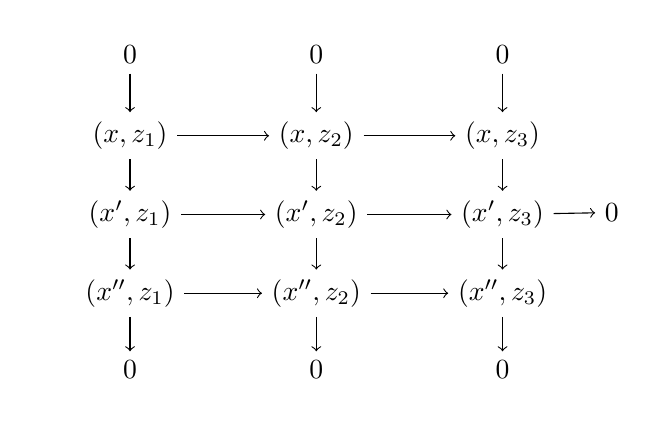
\begin{tikzpicture} \matrix (m) [matrix of math nodes, row sep={1cm,between origins}] {
		 &[0.5cm] 0 &[1cm] 0 &[1cm] 0 &[0.5cm]  \\ 
		 & \Hom(x, z_1) & \Hom(x, z_2) & \Hom(x, z_3) & \\ 
		 & \Hom(x', z_1) & \Hom(x', z_2) & \Hom(x', z_3) & 0 \\
		 & \Hom(x'', z_1) & \Hom(x'', z_2) & \Hom(x'', z_3) & \\
		& 0 & 0 & 0 & \\
		};
		\foreach \sourcerow/ \sourcecol / \targetrow / \targetcol in 
			{1/2/2/2, 1/3/2/3, 1/4/2/4, % first row of down arrows
			2/2/3/2, 2/3/3/3, 2/4/3/4,  % second row of down arrows
			3/2/4/2, 3/3/4/3, 3/4/4/4,  % third row of down arrows
			4/2/5/2, 4/3/5/3, 4/4/5/4,  % fourth row of down arrows
			%2/1/2/2, 
			2/2/2/3, 2/3/2/4, % first row of horiz arrows
			%3/1/3/2, 
			3/2/3/3, 3/3/3/4, 3/4/3/5, % second row of horiz arrows
			%4/1/4/2, 
			4/2/4/3, 4/3/4/4} % third row of horiz arrows
			\draw [->] (m-\sourcerow-\sourcecol) -- (m-\targetrow-\targetcol);
		\end{tikzpicture}
\]
The columns are exact because the objects $z_i$ are injective.  The middle row is exact because $x'$ is a primitive tensor.  A diagram chase shows that the map $\Hom(x,z_2) \ra \Hom(x,z_3)$ is surjective, and hence $\Hom((p \boxtimes q) \otimes x,-)$ is right exact, as required.

An argument of the same flavor, involving applications of parts (3) and (4) of Theorem~\ref{thm:DelignePrdtOverATCExists}, a resolution by a primitive tensor, and a diagram chase, shows that the action functor $(\cC \boxtimes \cD) \times (\cM \boxtimes \cN) \ra (\cM \boxtimes \cN)$ is exact.
\end{proof}


\subsection{Dual and functor bimodule categories} \label{sec:tc-bimodules}
\CDh{\S 3.4 $\checkmark$}

In this section we describe a number of operations on bimodule categories (flipping an action, twisting an action, taking a dual category, taking a functor category) and explain how they are related.  We then prove, in Proposition~\ref{prop:FunctorsAsATensorPdt}, that the relative Deligne tensor product can be expressed as a category of functors.  This fact will be crucial, in section~\ref{sec:df-modules}, in proving the $2$-dualizability of finite tensor categories.  Finally, we describe how the (right) dual of a (left) bimodule category can be interpreted as the category of modules over the double dual of an algebra object.  We will need this interpretation in giving, in section~\ref{sec:radfordftc}, a topological proof of the quadruple dual theorem.

\subsubsection{Flips and twists of bimodule categories} \label{sec:fliptwist}

Given a bimodule ${}_A M_B$ between ordinary algebras $A$ and $B$, we can flip the left $A$-action onto the right, producing a module $M_{A^\op \otimes B}$, or flip the right $B$-action onto the left, producing a module ${}_{A \otimes B^\op} M$, or flip both actions to the other side, producing the bimodule ${}_{B^\op} M_{A^\op}$.  More generally, if we have a bimodule of the form ${}_{A \otimes B} M_C$, we can flip just part of the action to obtain the bimodule ${}_A M_{B^\op \otimes C}$, or, of course, flip a bimodule ${}_A M_{B \otimes C}$ to a bimodule ${}_{A \otimes B^\op} M_C$.  The same operations work perfectly well on bimodule categories.

\begin{definition}
Let $\cC$, $\cD$, and $\cE$ be linear monoidal categories.  Given a bimodule category ${}_{\cC \boxtimes \cD} \cM_\cE$, the corresponding bimodule category ${}_{\cC} \cM_{\cD^\mp \boxtimes \cE}$ is called a \emph{flip} of ${}_{\cC \boxtimes \cD} \cM_\cE$.  Similarly, given a bimodule category ${}_\cC \cM_{\cD \boxtimes \cE}$, the corresponding bimodule category ${}_{\cC \boxtimes \cD^\mp} \cM_\cE$ is a flip of ${}_\cC \cM_{\cD \boxtimes \cE}$.
\end{definition}

\noindent We will be particularly interested in the bimodules obtained by flipping the actions of identity bimodule category ${}_\cC \cC_\cC$.  If we flip the right action to the left, then we have a module category ${}_{\cC \boxtimes \cC^\mp} \cC$; if we flip the left action to the right, then we have $\cC_{\cC^\mp \boxtimes \cC}$; if we flip both actions, we have a bimodule ${}_{\cC^\mp} \cC_{\cC^\mp}$, which is in fact precisely the identity bimodule of the category $\cC^\mp$.

Given a bimodule ${}_A M_B$ and a homomorphism of algebras $f: A' \rightarrow A$, we can twist, that is precompose, the $A$-action by the map $f$ to obtain an $A'$--$B$-bimodule denoted ${}_{\langle f \rangle} M$.  Similarly, given a homomorphism $g: B' \rightarrow B$, we can twist the right action to obtain an $A$--$B'$-bimodule denoted $M_{\langle g \rangle}$.  The same operations can be applied to bimodule categories.
\begin{definition}
Let $\cC$, $\cC'$, $\cD$, and $\cD'$ be linear monoidal categories, let ${}_\cC \cM_\cD$ be a bimodule category, and let $\cF: \cC' \rightarrow \cC$ and $\cG: \cD' \rightarrow \cD$ be monoidal functors.  The $\cC'$--$\cD$-bimodule obtained by precomposition with $\cF$ is called a \emph{twist} of ${}_\cC \cM_\cD$ and is denoted ${}_{\langle \cF \rangle} \cM$; in particular, the action on objects of ${}_{\langle \cF \rangle} \cM$ is $c' \cdot m \cdot d := \cF(c') \otimes m \otimes d$.  Similarly, a twist of the right action by a monoidal functor $\cG: \cD' \rightarrow \cD$ provides a $\cC$--$\cD'$-bimodule category denoted $\cM_{\langle \cG \rangle}$.
\end{definition}

Because of the relations ${}_{\langle f \rangle} A \otimes_A M \cong {}_{\langle f \rangle} M$ and ${}_{\langle f \rangle \langle g \rangle} M \cong {}_{\langle g \circ f \rangle} M$, there is a functor from the category of algebras and algebra homomorphisms to the 2-category of algebras, bimodules, and intertwiners: the functor is the identity on objects and sends a homomorphism to the corresponding twisted bimodule.  The analogous facts for bimodules, that ${}_{\langle \cF \rangle} \cC \boxtimes_\cC \cM \simeq {}_{\langle \cF \rangle} \cM$ and that ${}_{\langle \cF \rangle \langle \cG \rangle} \cM \simeq {}_{\langle \cF \otimes \cG \rangle} \cM$, ensure there is a functor from the 2-category of finite tensor categories, tensor functors, and tensor natural transformations, to the 3-category $\TC$ of finite tensor categories, finite bimodule categories, their functors, and their transformations: again the functor is the identity on objects and takes a functor to the corresponding twisted bimodule category.  Similarly, the fact that $\cM \boxtimes_\cD \cD_{\langle \cF \rangle} \simeq \cM_{\langle \cF \rangle}$ and $\cM_{\langle \cF \rangle \langle \cG \rangle} \simeq \cM_{\langle \cG \otimes \cF \rangle}$ ensures there is a functor from the 2-category of finite tensor categories to $\TC^{\op_1}$, the 3-category of tensor categories with the 1-morphisms reversed.
%\CD{I changed isomorphisms to equivalences in this paragraph, and in the next lemma.}

In section~\ref{sec:topquaddual}, the Radford bordism will provide an isomorphism between two twisted bimodules, and we will want to understand the significance of this isomorphism for the corresponding twisting functors.

\begin{lemma} \label{lem:BimoduleToFunctor}
Let $\cC$ and $\cD$ be linear monoidal categories and let $\cF: \cC \rightarrow \cD$ and $\cG: \cC \rightarrow \cD$ be monoidal functors.  The category of bimodule equivalences $\alpha: {}_\cC ({}_{\langle \cF \rangle} \cD)_\cD \rightarrow {}_\cC ({}_{\langle \cG \rangle} \cD)_\cD$ is equivalent to the category of pairs $(D, \varphi)$, where $D \in \cD$ is a tensor-invertible object and $\varphi$ is a monoidal natural isomorphism from $\cF$ to the monoidal functor $D^{-1} \otimes \cG(-) \otimes D$.
\end{lemma}
%!%\CD{changed tensor to monoidal here, and added the crucial monoidal conclusion. also change the statement}
%!%CD I haven't checked the proof of monoidal.
\begin{proof}
The functor $\alpha$ is in particular a right $\cD$-module functor from $\cD$ to $\cD$ and is therefore equivalent to the left multiplication functor $d \mapsto \alpha(1) \otimes d$.  The left $\cC$-module structure of $\alpha$ is a natural isomorphism $\alpha(c \cdot -) \cong c \cdot \alpha(-)$, that is $\alpha(\cF(c) \otimes -) \cong \cG(c) \otimes \alpha(-)$, which therefore provides a natural isomomorphism $a_{(c,-)}: \alpha(1) \otimes \cF(c) \otimes - \cong \cG(c) \otimes \alpha(1) \otimes -$.

The functor from bimodule equivalences to pairs takes the equivalence $\alpha$ to the pair $(D,\varphi)$ where $D:=\alpha(1)$ and $\varphi(c) := D^{-1} \otimes a_{(c,1)}$.  Note that $D$ is tensor-invertible because $\alpha$ is an equivalence.  Given a pair $(D,\varphi)$, the associated bimodule equivalence is $\alpha(d) := D \otimes d$ with left module structure map $D \otimes \varphi$.
\end{proof}


\subsubsection{Duals of bimodule categories}

Given a $\cC$--$\cD$-bimodule category, we can form a new bimodule category by twisting the $\cC$ and $\cD$ actions by the (say left) dual functors $\cC \ra \cC^\mop$ and $\cD \ra \cD^\mop$.  The resulting `dual' bimodule categories will play a central role in our dualizability analysis.

\begin{definition} \label{def:Dual_bimodule_notation}
Given a $\cC$--$\cD$-bimodule category $\cM$, the \emph{right dual} of $\cM$ is a $\cD$--$\cC$-bimodule category denoted $\cM^*$ and defined as follows.  The underlying linear category of $\cM^*$ is $\cM^\op$; an object $m \in \cM$ is denoted $m^*$ when viewed as an object of $\cM^*$.  The bimodule category structure on $\cM^*$ is given by
\[
d \cdot m^* \cdot c := ({}^* c \otimes m \otimes {}^* d)^*
\]
Similarly, the \emph{left dual} of $\cM$ is the $\cD$--$\cC$-bimodule category ${}^* \cM$ with underlying category $\cM^\op$ and actions
\[
d \cdot {}^* m \cdot c := {}^* (c^* \otimes m \otimes d^*).
\]
\end{definition}

\noindent The terminology, referring to these bimodule categories as duals, will be justified later in two ways: first, we will see that the bimodule categories are categories of functors into the base tensor categories, therefore are linear duals in the classical sense, and second, we will see that these bimodule categories are adjoint bimodules.  

There is a quite important, potentially confusing, subtlety arising here, namely that the process of taking a dual bimodule category does not commute with the process of flipping an action between the left and the right of a bimodule; this issue is probably responsible for some of the inaccuracies in the literature concerning dual bimodules.  Because flipping an action changes $\cC$ to $\cC^\mp$, and a left dual in $\cC$ is a right dual in $\cC^\mp$, the failure of commutativity is in fact a double dual.
\begin{lemma} \label{lemma:DualTwist}
The $\cD$--$\cC$-bimodule flip of the right dual of the right $(\cC^\mp \boxtimes \cD)$-module flip of a $\cC$--$\cD$-bimodule category $\cM$ is the right twist by the right double dual functor of the right dual of the bimodule category $\cM$; that is,
\[
{}_\cD ((\cM_{\cC^\mp \boxtimes \cD})^*)_\cC \simeq (({}_\cC \cM_\cD)^*)_{\langle \mathfrak{r r} \rangle},
\]
where $\mathfrak{r}$ denotes the right dual functor.  Similarly
\[
{}_\cD (({}_{\cC \boxtimes \cD^\mp}\cM)^*)_\cC \simeq {}_{\langle \mathfrak{r r} \rangle}(({}_\cC \cM_\cD)^*).
\]

\end{lemma}
\noindent The proof is simply chasing carefully through the definitions.  Analogous formulas hold for left dual categories.
\CD{Double check these formulas.}

We will need to know that the duals of exact module categories are exact.  (Recall that a $\cC$-module category $\cM$ is called exact if $p \otimes m \in M$ is projective whenever $p \in \cC$ is projective.)  Toward that end, we first prove an auxiliary result concerning exactness of contravariantly, monoidally-oppositely twisted modules.  For a left $\cC$-module $\cM$ and $\cF: \cC \rightarrow \cC^\mop$ a tensor equivalence, let $\cM^{\op(\cF)}$ denote the right $\cC$-module with underlying linear category $\cM^\op$ and action $m \cdot c := F(c) \otimes m$.
\begin{lemma}
Let $\cC$ be a finite tensor category, and $\cM$ an exact left $\cC$-module category.  For any tensor equivalence $\cF: \cC \rightarrow \cC^\mop$, the right $\cC$-module category $\cM^{\op(\cF)}$ is exact.
\end{lemma}
\begin{proof}
Recall from Theorem~\ref{Thm:ExactModCatOmnibus}, using Example~\ref{ex:exactness}, that projective objects in $\cC$ are injective and vice versa, and similarly for objects in $\cM$.  Consider an object $m \in \cM^{\op(\cF)}$ and a projective object $p \in \cC$.  Because $p \in \cC$ is projective, it follows that $\cF(p)$ is projective as an object of $\cC^\mop$, therefore injective as an object of $\cC^\mop$, therefore, by reversing the arrows, projective as an object of $\cC^\mp$.  By the exactness of $\cM$, it follows that $\cF(p) \otimes m$ is projective as an object of $\cM$, therefore injective as an object of $\cM$, and then, by reversing arrows, projective as an object of $\cM^{\op(\cF)}$, as required.
\end{proof}

\noindent Applying this lemma with the functor $\cF$ being an appropriate combination of duals (taking account of Lemma~\ref{lemma:DualTwist}) provides the desired result:

\begin{corollary} \label{cor:adjoint-exactness}
Let $\cC$ and $\cD$ be finite tensor categories and $\cM$ an exact $\cC$--$\cD$-bimodule category.  The dual bimodule categories $\cM^*$ and ${}^* \cM$ are exact $\cD$--$\cC$-bimodule categories.
\end{corollary}

\subsubsection{The dual bimodule category is the functor dual}

The dual of a finite-dimensional $k$-vector space $V$ can of course be characterized as a dual object in the category of vector spaces, but it can also be constructed explicitly as the linear dual vector space $\Hom_k(V,k)$.  For an ordinary bimodule ${}_A M_B$ (which is finitely generated and projective both as an $A$-module and as a $B$-module), there are left and right adjoints, which may be characterized as adjoint morphisms or may be constructed explicitly as the left and right linear duals $\Hom_A(M,A)$ and $\Hom_B(M,B)$.  The situation for bimodule categories is analogous, as we will see later on: for a bimodule category ${}_\cC \cM_\cD$, the left and right adjoint bimodule categories may be characterized abstractly or may be constructed explicitly as the linear functor dual categories $\Fun_\cC(\cM,\cC)$ and $\Fun_\cD(\cM,\cD)$, respectively.  

We now show that the left and right dual bimodule categories ${}^* \cM$ and $\cM^*$, defined above, are equivalent to the functor left and right dual categories $\Fun_\cC(\cM,\cC)$ and $\Fun_\cD(\cM,\cD)$, respectively; the dual bimodule categories will therefore provide alternative explicit realizations of adjoint bimodules.

We will first show that the dual of a functor bimodule category is itself a functor bimodule category.  For that we will need to temporarily break from our convention and consider functors that are not necessarily right exact.  Given bimodule categories ${}_\cC \cM_\cD$ and ${}_{\cC} \cN_{\cE}$, let ${}_{\cD} \Fun^L_{\cC}(\cN,\cM)_{\cE}$ denote the $\cD$--$\cE$-bimodule category of left exact (not necessarily right exact) $\overline{Vect}_k$-enriched $\cC$-module functors.  Bimodule categories of left exact right-module functors will be denoted similarly.

\begin{lemma}
Let ${}_\cC \cM_\cD$ and ${}_\cC \cN_\cE$ be finite bimodule categories between finite tensor categories.  Taking the right adjoint of a functor is an equivalence of $\cD$--$\cE$-bimodule categories from $\Fun_\cC(\cM,\cN)$ to ${}^* \Fun^L_\cC(\cN,\cM)$.  Similarly, if ${}_\cM \cM_\cD$ and ${}_\cE \cN_\cD$ are finite bimodule categories, then taking the right adjoint is an equivalence from ${}^* \Fun_\cD(\cM,\cN)$ to $\Fun^L_\cD(\cN,\cM)$.
\end{lemma}
\begin{proof}
Note that the right adjoint of a $\cC$-module functor from $\cM$ to $\cN$ is a linear functor from $\cN$ to $\cM$, which by Lemma~\ref{lma:module-adjoint} has a canonical $\cC$-module structure.  Taking right adjoints is certainly an equivalence of linear categories, with inverse taking left adjoints.  It therefore suffices to check that this process preserves the $\cD$--$\cE$-bimodule structure.  Observe that in any finite tensor category, we have the following two sequences of adjunctions of tensor product functors:
\begin{alignat*}{5}
	& x^* \otimes (-)  \quad & &  \dashv \quad &&  \quad x \otimes (-)  \quad &&  \dashv &&  \quad {}^*x \otimes (-), \\
	& (-) \otimes {}^* y  \quad & &  \dashv \quad &&  \quad (-) \otimes y  \quad &&  \dashv &&  \quad (-) \otimes y^*. 
\end{alignat*}  
The same adjunctions hold when the tensor represents the action on a module category.  For $\cF \in \Fun_{\cC}(\cM,\cN)$, the left $\cD$ action is by definition $(d \cdot \cF)(m) = \cF(m \otimes d)$.  The right adjoint of the composite functor $\cF(- \otimes d)$ is therefore $\cF^R(-) \otimes d^*$, as required.  The right $\cE$ action is similar, as is the case of right module functors.
\end{proof}


We can now prove the desired equivalence between the dual and functor categories.
\begin{proposition} \label{prop:dual-formula-for-adjoints}
Given a finite bimodule category ${}_\cC \cM_\cD$ between finite tensor categories, there are equivalences ${}^* \cM \simeq \Fun_\cC(\cM,\cC)$ and $\cM^* \simeq \Fun_\cD(\cM,\cD)$.  The first equivalence takes an object ${}^* m \in {}^* \cM$ to the left adjoint of the functor $c \mapsto c \otimes m$; the second equivalence takes an object $m^* \in \cM^*$ to the left adjoint of the functor $d \mapsto m \otimes d$.
\end{proposition}
\begin{proof}
By the previous lemma, there is an equivalence between $\Fun_\cC(\cM,\cC)$ and ${}^* \Fun^L_\cC(\cC,\cM)$.  The category of all (not necessarily right or left exact) $\cC$-module functors from $\cC$ to $\cM$ is certainly equivalent to $\cM$.  However, because $\cC$ is finite tensor, it is exact over itself (as in Example~\ref{ex:exactness}), and therefore all $\cC$-module functors from it are exact, in particular left exact.  The other equivalence is obtained in the same fashion.
\end{proof}


\subsubsection{The relative Deligne tensor product as a functor category}

In constructing the duality between a (finite-dimensional) vector space $V$ and the linear dual $\Hom_k(V,k)$, it is convenient to know that that $\Hom_k(V,k) \otimes V \cong \Hom_k(V,V)$ (or more generally that $\Hom_k(V,k) \otimes W \cong \Hom_k(V,W)$): the coevaluation of the duality can then be expressed simply as $1 \mapsto \id_V$.  Analogously, in constructing the adjoint of an (appropriately finite) bimodule ${}_A M_B$, it is convenient to know that $\Hom_A(M,A) \otimes_A M \cong \Hom_A(M,M)$ (more generally, that $\Hom_A(M,A) \otimes_A N \cong \Hom_A(M,N)$) and that $M \otimes_B \Hom_B(M,B) \cong \Hom_B(M,M)$ (more generally, that $N \otimes_B \Hom_B(M,B) \cong \Hom_B(M,N)$).  Our next endeavor is to prove the analogous facts, namely $\Fun_\cC(\cM,\cC) \boxtimes_\cC \cN \simeq \Fun_\cC(\cM,\cN)$ and $\cN \boxtimes_\cD \Fun_\cD(\cM,\cD) \simeq \Fun_\cD(\cM,\cN)$, for bimodule categories.  When $\cC$ and $\cD$ are finite semisimple tensor categories and ${}_\cC \cM_\cD$ is a finite semisimple bimodule category, these facts are useful, but in the end merely a convenience, for constructing the adjoint of the bimodule category ${}_\cC \cM_\cD$.  However, when $\cC$ and $\cD$ are not semisimple, the reexpression of the relative tensor as a functor category is completely indispensable in constructing the necessary adjoints, and therefore for proving our dualizability results.  (The expression of a relative tensor product as a functor category allows the construction of functors into the relative tensor product, whose universal definition a priori only characterizes functors out.)

As discussed in Remark~\ref{rmk:Deligne_pdt_as_mod_functor} below, the following proposition and corollary are closely related to  \cite[Prop. 3.5 and Rmk. 3.6]{0909.3140} and \cite[Thm. 3.20]{0911.4979}.
\begin{proposition} \label{prop:FunctorsAsATensorPdt}
Let $\cC$, $\cD$, and $\cE$ be finite tensor categories and ${}_\cC \cM_\cD$ and ${}_\cC \cN_\cE$ finite bimodule categories.  The balanced functor $\Fun_\cC(\cM,\cC) \times \cN \ra \Fun_\cC(\cM,\cN)$, $(\cF,n) \mapsto \cF(-) \otimes n$, induces an equivalence, of $\cD$--$\cE$-bimodule categories,
\[
		\Fun_\cC(\cM, \cC) \boxtimes_\cC \cN \simeq \Fun_\cC(\cM,\cN).
\]
Here $\Fun_\cC$ denotes the category of (right exact) $\cC$-module functors.  If instead the bimodule categories are ${}_\cC \cM_\cD$ and ${}_\cE \cN_\cD$, then the analogous balanced functor induces an $\cE$--$\cC$-bimodule category equivalence
\[
\cN \boxtimes_\cD \Fun_{\cD}(\cM,\cD) \simeq \Fun_{\cD}(\cM,\cN).
\]
\end{proposition}

\begin{proof}
We focus on the first equivalence, as the second is analogous.  The functor induced by the balanced functor is certainly a bimodule functor, so it suffices to see that it is an equivalence of linear categories.  We prove that $\Fun_\cC(\cM, \cC) \boxtimes_\cC \cN$ and $\Fun_\cC(\cM,\cN)$ are both equivalent to a category of the form $\Mod{A}{B}(\cC)$, by equivalences intertwining the functor in question.

Using Theorem~\ref{thm:EGNO2.11.6}, choose algebra objects $A \in \cC$ and $B \in \cC$ and equivalences $\cM \simeq \Mod{}{A}(\cC)$ and $\cN \simeq \Mod{}{B}(\cC)$.  The functor $\tau: \Mod{A}{B}(\cC) \rightarrow \Fun_\cC(\cM,\cN)$, given by $\tau(M) = - \otimes_A M$, is an equivalence, as we will see presently and as observed in \cite[Prop 2.12.2]{EGNO}.  A functor $\cF \in \Fun_\cC(\cM,\cN)$ is naturally equivalent to the functor $\tau(\cF(A)) = - \otimes_A \cF(A)$, so $\tau$ is essentially surjective.  (To see this note that $\cF$ and $\tau(\cF(A))$ agree on free $A$-modules, and any object $M \in \cM \simeq \Mod{}{A}(\cC)$ is the canonical coequalizer $\textrm{coeq}_\cC(M \otimes A \leftleftarrows M \otimes A \otimes A)$ of free $A$-modules.)  The functor $\tau$ is evidently fully faithful.  A special case of the equivalence $\tau$ gives an equivalence $\Mod{A}{}(\cC) \simeq \Fun_\cC(\cM,\cC)$.  The equivalence between $\Fun_\cC(\cM, \cC) \boxtimes_\cC \cN$ and $\Mod{A}{B}(\cC)$ now follows from Theorem~\ref{thm:DelignePrdtOverATCExists}.
\end{proof}

\begin{corollary} \label{cor:tensasfunct}
For ${}_\cD \cM_\cC$ and ${}_\cC \cN_\cE$ finite bimodule categories over finite tensor categories, there are equivalences of $\cD$--$\cE$-bimodule categories
\begin{align*}
\cM \boxtimes_\cC \cN &\simeq \Fun_{\mod{\cC}{}}(\cM^*,\cN), \\
\cM \boxtimes_\cC \cN &\simeq \Fun_{\mod{}{\cC}}(\cM,{}^* \cN).
\end{align*}
\end{corollary}
\begin{proof}
By Propositions \ref{prop:dual-formula-for-adjoints} and \ref{prop:FunctorsAsATensorPdt}, we have
\[
\cM \boxtimes_\cC \cN \simeq {}^*(\cM^*) \boxtimes_\cC \cN \simeq \Fun_{\mod{\cC}{}}(\cM^*,\cC) \boxtimes_\cC \cN \simeq \Fun_{\mod{\cC}{}}(\cM^*,\cN).
\]
Similarly
\[
\cM \boxtimes_\cC \cN \simeq \cM \boxtimes_\cC ({}^* \cN)^* \simeq \cM \boxtimes_\cC \Fun_{\mod{}{\cC}}(\cN,\cC) \simeq \Fun_{\mod{}{\cC}}(\cM,{}^* \cN).\qedhere
\]
\end{proof}

\begin{remark} \label{rmk:Deligne_pdt_as_mod_functor}
This corollary is a correction of \cite[Remark 3.6]{0909.3140} and \cite[Thm. 3.20]{0911.4979}, both of which are off by a twist by a double dual functor.\footnote{Note also that, even appropriately corrected, the proof of \cite[Thm 3.20]{0911.4979} is incomplete.  For instance, it uses \cite[Lemma 3.21]{0911.4979}, which is false.  A counterexample to that Lemma is given by $\cC = \Vect_G$, the category of $G$-graded vector spaces for a finite group $G$, and $\cM = \cN = \Vect$.  The Lemma would have $\Vect \boxtimes \Vect \simeq \Vect$ equivalent to $\Fun_{\Vect_G}(\Vect,\Vect) \simeq \Rep(G)$; no such equivalence exists unless $G$ is the trivial group.} \CD{Check footnote against the relevant version of Greenough, and make sure bib reference is to that version only.}
\end{remark} %!%CDNC


\subsubsection{Dual bimodule categories as modules over a double dual}

By Theorem \ref{thm:EGNO2.11.6}, any module category ${}_\cC \cM$ can be expressed as a category of modules $\Mod{}{A}(\cC)$ for an algebra object $A \in \cC$.  We now describe explicitly how the left and right duals of the module category ${}_\cC \cM$ can themselves be expressed as module categories.  The following lemma and its corollary are based on calculations in \cite[\S 3]{MR2097289}.

\begin{lemma}\label{lem:dualing-amod}
Let $A \in \cC$ and $B \in \cC$ be algebra objects in a finite tensor category $\cC$, and let $M \in \cC$ be an $A$--$B$-bimodule object.  The objects ${}^{**} A$ and $B^{**}$ are naturally algebra objects, the object $M^*$ is naturally a $B^{**}$--$A$-bimodule object, and the object ${}^* M$ is naturally a $B$--${}^{**} A$-bimodule object.  Moreover, the left and right duals provide equivalences of linear categories:
\begin{equation*}
\begin{array}{ccccc}
	\Mod{B^{**}}{A}(\cC) &\simeq& \Mod{A}{B}(\cC) &\simeq& \Mod{B}{{}^{**}A}(\cC) \\
	M^* &\leftmapsto& M &\rightmapsto& {}^* M
\end{array}
\end{equation*}
\end{lemma}

\begin{proof}
The left and right double dual functors are tensor equivalences, thus take algebra objects to algebra objects.  The right dual of the action map $\mu: A \otimes M \otimes B \rightarrow M$ is $\mu^*: M^* \rightarrow B^* \otimes M^* \otimes A^*$; taking the left adjoint of the functor $B^* \otimes - \otimes A^*$, we have a map $B^{**} \otimes M^* \otimes A \rightarrow M^*$, as desired.  The action on ${}^* M$ is similar, and it is clear that the duals provide equivalences as stated.
\end{proof}

\begin{corollary} \label{cor:dualamod}
Let $A \in \cC$ be an algebra object in a finite tensor category $\cC$.  There is an equivalence of right $\cC$-module categories
	\begin{align*}
		(\Mod{}{A}(\cC))^* & \simeq \Mod{A^{**}}{}(\cC) \\
		(L)^* & \mapsto L^*.
	\end{align*}
Here $(L)^*$ denotes the object $L$ viewed as an object of $(\Mod{}{A}(\cC))^*$ as in Definition~\ref{def:Dual_bimodule_notation}, whereas $L^*$ denotes the right dual of $L$ as an object of $\cC$.  There are analogous equivalences of $\cC$-module categories
\begin{align*}
(\Mod{A}{}(\cC))^* &\simeq \Mod{}{A}(\cC), \\
{}^*(\Mod{}{A}(\cC)) &\simeq \Mod{A}{}(\cC), \\
{}^*(\Mod{A}{}(\cC)) &\simeq \Mod{}{{}^{**}A}(\cC).
\end{align*}
\end{corollary}

\subsection{Separable module categories and separable tensor categories} \label{sec:tc-separable}
\CDh{\S 3.5 $\checkmark$}

In the previous section, we laid the foundation for understanding when a bimodule category ${}_\cC \cM_\cD$ has adjoints.  However, because we are studying dualizability in a 3-category, we care not only about whether a bimodule category has adjoints, but also whether the units and counits of those adjunctions themselves have adjoints---in other words, we need two additional layers of dualizability above the bimodule category itself.  For inspiration, we can recall the situation governing the 2-dualizability of ordinary algebras: a finite-dimensional $k$-algebra $A$ is 2-dualizable if and only if it is projective as an $A \otimes A^\op$-module.  This projectivity condition is called `separability' and is equivalent to requiring that the multiplication map $\mu: A \otimes A \rightarrow A$ splits as an $A$--$A$-bimodule map.  

Recall that the bimodule category ${}_\cC \cM_\cD$ can be written (as a $\cC$-module) as $\Mod{}{A}(\cC)$ for an algebra object $A \in \cC$, or (as a $\cD$-module) as $\Mod{B}{}(\cD)$ for an algebra object $B \in \cD$.  These expressions of bimodule categories as categories of modules for algebra objects invites the following definitions.
\begin{definition}
An algebra object $A \in \cC$ in a semisimple finite tensor category $\cC$ is \emph{separable} if the multiplication $\mu: A \otimes A \ra A$ splits as an $A$--$A$-bimodule map, or equivalently if $A$ is projective as an $A$--$A$-bimodule.
\end{definition}
\noindent (That these two definitions of separability of an algebra object are equivalent is seen as follows: the projectivity condition certainly implies the splitting condition; conversely, because $\cC$ is semisimple, the unit $1 \in \cC$ is projective, which implies that $A \otimes A$ is projective as an $A$--$A$-bimodule, and using the splitting this implies that $A$ is projective as an $A$--$A$-bimodule.)
\begin{definition}
A finite left module category ${}_\cC \cM$ over a semisimple finite tensor category $\cC$ is \emph{separable} if it is equivalent as a $\cC$-module to the category of modules $\Mod{}{A}(\cC)$ over a separable algebra object $A \in \cC$.  Similarly, a finite right module category $\cM_\cD$ is separable if it is equivalent to $\Mod{B}{}(\cD)$ for a separable algebra object $B \in \cD$.  A finite bimodule category ${}_\cC \cM_\cD$ is separable if it is separable as a $\cC$-module and it is separable as a $\cD$-module.
\end{definition}
\noindent We will see later, in Section~\ref{sec:separableisfd}, that this separability condition is, as hoped, exactly what is needed to ensure a bimodule category is maximally dualizable.  

In this section, we prove two crucial properties of separable module categories, namely (1) that a module category is separable if and only if its category of endofunctors is semisimple and (2) that the relative Deligne tensor product of two separable bimodule categories is a separable bimodule category.  The second is a generalization to arbitrary fields of Etingof--Nikshych--Ostrik's theorem, over an algebraically closed field of characteristic zero, that a functor category between finite semisimple module categories is semisimple~\cite[Theorem 2.16]{MR2183279}.  Using a simple case of the second result, the first result provides a generalization to arbitrary fields of M\"uger's theorem, over algebraically closed fields, that the Drinfeld center of a finite semisimple tensor category of nonzero global dimension is semisimple~\cite[Theorem 3.16]{MR1966525}.    These results are inspired by a suggestion of Ostrik and by results in \cite[\S 2.4]{MR3039775} in characteristic zero.  The reader unconcerned with finite characteristic can safely skip this and the next section, consulting Corollary~\ref{cor:charzerosep} and Proposition~\ref{prop:SSModuleCatsAreSep} for characterizations of separability in the characteristic zero case, and keeping in mind ENO's aforementioned theorem at appropriate moments in Section~\ref{sec:separableisfd}.


\CD{Did Muger use sphericality?}

\begin{remark}
It is well known that naive generalizations, to arbitrary fields, of M\"uger's and ENO's results are false.  The importance of nonzero global dimension is clear from the statement of M\"uger's theorem, and Kuperberg observed that, over a non-perfect field, inseparable field extensions could yield non-semisimple composites \cite[Section 5]{MR1995781}.
\end{remark} \CD{Reconsider this remark}


%!%CDcheckmugerstatement; also muger was arbitrary char, right?
%\CD{Previous discussion made it seem like muger was char zero}

\subsubsection{Separability and semisimplicity} \label{sec:sepandsemi}

Over a perfect field (for instance, a finite field, an algebraically closed field, or a field of characteristic zero), an algebra $A$ is separable if and only if it is finite-dimensional semisimple; over an arbitrary field, separability is a stronger condition than finite-dimensional semisimplicity \cite[Ch.~2]{MR0280479}.  The corresponding statements hold for linear categories: over a perfect field, a finite $\Vect$-module category is separable if and only if it is finite semisimple, while over an arbitrary field separability merely implies finite semisimplicity. \CSP{I added a reference for classical separability} %!%CD
In general, a finite linear category $\cL$ is separable (as a $\Vect$-module) if and only if for all simple objects $S \in \cL$, the extension from the base field to the center of the division ring of endomorphisms of $S$ is a finite separable field extension.  In other words, a finite linear category is separable if and only if it remains semisimple after arbitrary base changes---we refer to this condition as `absolute semisimplicity' and for clarity use that term instead of `separable as a $\Vect$-module'. \NS{Classical references?} %!%CD 
%!%This is the first moment that base change has been discussed.  We should say what base change means, especially to highlight that there is an idempotent completion happening.

For tensor categories $\cC$ other than $\Vect$, a separable $\cC$-module is still semisimple:
\begin{proposition} \label{prop:sepmodissemi}
A separable module category ${}_\cC \cM$, over any finite semisimple tensor category $\cC$, is semisimple.
\end{proposition}
\begin{proof}
It suffices to show that all objects of $\cM$ are projective.  Express ${}_\cC \cM$ as $\Mod{}{A}(\cC)$ for a separable algebra object $A$.  Because $\cC$ is semisimple, the unit $1 \in \cC$ is projective, which implies that $A \in \Mod{}{A}(\cC)$ is projective, which in turn implies any free right $A$-module is projective in $\Mod{}{A}(\cC)$.  Any object $M \in \Mod{}{A}(\cC)$ is a summand of a free $A$-module, via $M \otimes_A A \xra{\id \otimes s} M \otimes_A (A \otimes A)$ where $s$ is the bimodule splitting, and therefore is projective as required.
\end{proof}
\noindent Thus, by Example~\ref{eg:semiexact}, separable module categories are exact.

We can moreover characterize the separability of $\cC$-module categories in terms of a semisimplicity condition, though on the category of endomorphisms.
\begin{theorem} \label{thm:SepModCats}
Let $\cC$ be a finite semisimple tensor category and let ${}_\cC \cM$ be a finite $\cC$-module category.  The following conditions are equivalent:
\begin{enumerate}
\item the module category ${}_\cC \cM$ is separable,
\item the linear category $\Fun_{\cC}(\cM,\cM)$ is semisimple.  
\end{enumerate}
The same statements hold for right $\cC$-module categories.
\end{theorem}
\begin{proof}
Stitching together Theorem~\ref{thm:DelignePrdtOverATCExists}, Corollary~\ref{cor:tensasfunct}, and Corollary~\ref{cor:dualamod}, we can write ${}_\cC \cM$ as $\Mod{}{A}(\cC)$ and $\Fun_{\cC}(\cM,\cM)$ as $\Mod{A}{A}(\cC)$ for an algebra object $A \in \cC$.  

If we assume $\Mod{A}{A}(\cC)$ is semisimple, then all its objects are projective; in particular $A$ is projective as a bimodule object, and so ${}_\cC \cM$ is separable.  Conversely, assume that $A$ is projective as an $A$--$A$-bimodule, in other words that the unit $1 \in \Fun_{\cC}(\cM,\cM)$ is projective.  Because $\Fun_{\cC}(\cM,\cM)$ is rigid (by item (6) of Theorem~\ref{Thm:ExactModCatOmnibus}), for any object $F \in \Fun_{\cC}(\cM,\cM)$, the functor $\Hom(F,-) \simeq \Hom(1,{}^* F \otimes -)$ is right exact and so $F$ is projective; thus the functor category is semisimple, as required.
\end{proof}

%\CD{Removed identity functor projective --- general triviality, not used?}


\subsubsection{Separable bimodules compose}

Over an algebraically closed field of characteristic zero, finite semisimple bimodule categories over finite semisimple tensor categories have the excellent feature than they compose, that is the relative Deligne tensor of two such is again of the same type---this is a reformulation of~\cite[Theorem 2.16]{MR2183279}.  We generalize that result to an arbitrary field.
\begin{theorem} \label{thm:compositeOfSep}
Let ${}_\cB \cM_\cC$ and ${}_\cC \cN_\cD$ be separable bimodule categories over finite semisimple tensor categories.  The relative Deligne tensor product ${}_{\cB} \cM \boxtimes_\cC \cN_\cD$ is a separable bimodule category.
\end{theorem}

\begin{proof}
We prove that the product is separable as a $\cB$-module; separability as a $\cD$-module is similar.  Choose separable algebra objects $A \in \cB$ and $C \in \cC$ and an algebra object $B \in \cC$, such that
\begin{itemize}
\item $\cM \simeq \Mod{}{A}(\cB)$ as left $\cB$-module categories
\item $\cM \simeq \Mod{B}{}(\cC)$ as right $\cC$-module categories
\item $\cN \simeq \Mod{}{C}(\cC)$ as left $\cC$-module categories
\end{itemize}
It follows that $\cM \boxtimes_{\cC} \cN \simeq \Mod{B}{C}(\cC)$.  We suppress all four of these equivalences in what follows, freely transporting objects from $\Mod{}{A}(\cB)$ to $\cM$ to $\Mod{B}{}(\cC)$, and such, without comment or notation.  For instance, ``$A$" refers both to the algebra object $A \in \cB$ and as usual to the corresponding module object $A_A \in \Mod{}{A}(\cB)$, and therefore also to an object $A \in \cM$ and to a module object ${}_B A \in \Mod{B}{}(\cC)$.  We will however sometimes indicate by the notation $[-]_\cE$ when we forget to an ambient tensor category $\cE$.  Thus, for instance, the expression $[A]_\cC$ would be the object of $\cC$ obtained by forgetting the left $B$-action on ${}_B A \in \Mod{B}{}(\cC)$.  Moreover, we will drop the subscript from $[-]$ when the ambient tensor category in question is clear from context.

To see that the product $\cM \boxtimes_\cC \cN \simeq \Mod{B}{C}(\cC)$ is separable, we need to identify it (as a left $\cB$-module) as a category of modules for a separable algebra object in $\cB$.  As a linear category, the product is certainly the category of algebras (that is, modules) for the monad $T := - \otimes C : \cM \ra \cM$.  Here, a priori, $T$ is a monad on $\cM$ considered as a linear category (that is, $T$ is an algebra object in $\Fun(\cM,\cM)$).  However because the left $\cB$-action commutes with the right $\cC$-action on $\cM$, in fact $T$ is a monad on $\cM$ considered as a left $\cB$-module (that is, $T$ is an algebra object in $\Fun_\cB(\cM,\cM)$); the product $\cM \boxtimes_\cC \cN$ is, as a left $\cB$-module, the category of algebras for the monad $T$ acting on $\cM$ as a left $\cB$-module.  

We can reformulate the category of algebras for this monad as a category of modules for an algebra object.  We give $[T(A)]_\cB$ the structure of an algebra objects in $\cB$, as follows.  The multiplication is the composite
\[
[T(A)] \otimes [T(A)] \cong [[T(A)] \otimes T(A)] \cong [T([T(A)] \otimes A)] \xra{[T(\alpha)]} [T(T(A))] \ra [T(A)]
\]
The first isomorphism exists because the forgetful functor from $\Mod{}{A}(\cB)$ to $\cB$ is left $\cB$-linear.  The second isomorphism comes from the left $\cB$-linearity of the monad $T$.  For any object $M \in \cM$, the object $[M] \in \cB$ is a right $A$-module; the action map $[M] \otimes A \ra [M]$ (in $\cB$) is a right $A$-module map, so there is a corresponding morphism $[M] \otimes A \ra M$ in $\cM$.  In particular, there is the morphism $\alpha: [T(A)] \otimes A \ra T(A)$ used in the third map above.  The fourth map is the composition of the monad.  The unit of the algebra object $[T(A)]$ is simply the composite $1 \ra A \ra [T(A)]$, where the second map is obtained, from the unit $A \ra T(A)$ of the monad, by forgetting to $\cB$.

We know that ${}_\cB \cM \boxtimes_\cC \cN$ is the category of $T$-algebras in ${}_\cB (\Mod{}{A}(\cB))$; we now check that that this category of $T$-algebras is precisely ${}_\cB (\Mod{}{[T(A)]}(\cB))$ the left $\cB$-module category of right $[T(A)]$-modules in $\cB$.  As we now work exclusively within $\cB$, we will dispense with the $[-]$ notation.  Observe that because the monad $T$ is right exact and left $\cB$-linear, there is, for any object $M \in \Mod{}{A}(\cB)$, an isomorphism $T(M) \cong M \otimes_A T(A)$.  Therefore, on the one hand, given a $T$-algebra in $\Mod{}{A}(\cB)$, we have a (right $A$-module) action map $M \otimes_A T(A) \ra M$, which determines a (right $A$-module) action map $M \otimes T(A) \ra M$ by precomposition along $M \otimes T(A) \ra M \otimes_A T(A)$.  On the other hand, the unit map $A \ra T(A)$ is a homomorphism of algebra objects in $\cB$, and it follows that every action map $M \otimes T(A) \ra M$ is $A$-balanced and so determines an action map $M \otimes_A T(A) \ra M$, that is, an $T$-algebra structure.

It remains only to check that $T(A) \in \cB$ is a separable algebra object.  Pick bimodule splittings $s: A \ra A \otimes A$ and $\sigma: C \ra C \otimes C$ of the multiplication maps of $A$ and $C$.  These combine to provide a bimodule splitting of the multiplication map on $T(A)$, as required:
\[
T(A) \xra{\id_A \otimes \sigma} T(T(A)) \cong T(T(A) \otimes_A A) \xra{T(\id_{T(A)} \otimes_A s)} T(T(A) \otimes A) \cong T(A) \otimes T(A). \qedhere
\]

\end{proof} %\CD That proof didn't use the separability of B, right?


\begin{corollary} \label{cor:funsemi}
For absolutely semisimple, separable $\cC$-modules ${}_\cC \cM$ and ${}_\cC \cN$ over a finite semisimple tensor category $\cC$, the functor category $\Fun_{\cC}(\cM,\cN)$ is absolutely semisimple.
\end{corollary}
%!% \CD{Does $\cC$-separable imply $\Vect$-separable? If so, drop absolute semisimple assumption.  But seems not.}

\begin{corollary} \label{cor:septc}
Assume the base field is perfect.  Finite semisimple tensor categories, finite separable bimodule categories, bimodule functors, and bimodule transformations, form a symmetric monoidal sub-3-category $\TCss$ of $\TC$.
\end{corollary}
\nid Because of the perfection assumption, every finite semisimple linear category is absolutely semisimple---this ensures, for instance, that the ordinary Deligne tensor product of semisimple tensor categories is again semisimple.

%\noindent Here, the absolute semisimplicity assumptions are necessary for ensuring, for instance, that the symmetric monoidal product of two separable bimodules is again separable.  
\CD{**Should we include a proof of this corollary?}
%!% Check ordinary product of separable is separable.

As mentioned, we will see that separable bimodule categories ${}_\cC \cM_\cD$ are maximally dualizable.  What we really care about, though, is the dualizability of tensor categories.  Thus, what concerns us most is the separability of the bimodules ${}_{\cC \boxtimes \cC^\mp} \cC$ and $\cC_{\cC^\mp \boxtimes \cC}$ arising in the 1-dualizability of $\cC$.  This suggests the following definition.
\begin{definition}
A finite semisimple tensor category $\cC$ over a perfect field is \emph{separable} if it is separable as a $\cC \boxtimes \cC^\mp$--$\Vect$-bimodule.
\end{definition}
\nid The full sub-3-category of $\TCss$ on the separable tensor categories will be of special significance: in Section~\ref{sec:separableisfd} we will prove it is a fully dualizable 3-category.
\begin{definition}
The \emph{3-category of separable tensor categories} $\TCsep$ (over a perfect field) has objects the separable tensor categories, morphisms the finite separable bimodule categories, 2-morphisms the bimodule functors, and 3-morphisms the bimodule transformations.
\end{definition}

Recall that the (Drinfeld) center of a finite tensor category $\cC$ is by definition the linear category $\cZ(\cC) := \Fun_{\cC \boxtimes \cC^\mp}(\cC,\cC)$.  By Theorem~\ref{thm:compositeOfSep}, if $\cC$ is absolutely semisimple, then $\cC \boxtimes \cC^\mp$ is absolutely semisimple.  As a corollary of Theorem~\ref{thm:SepModCats}, we now have the generalization of M\"uger's theorem on the semisimplicity of Drinfeld centers.
\begin{corollary} \label{cor:Sep=semisimplecenter}
Let $\cC$ be a finite semisimple tensor category over a perfect field.  The following conditions are equivalent:
\begin{enumerate}
\item the tensor category $\cC$ is separable,
\item the Drinfeld center $\cZ(\cC)$ is semisimple.
\end{enumerate}
\end{corollary}


\subsection{Separability and global dimension} \label{sec:tc-fusion}
\CDh{\S 3.6 $\checkmark$}


In this section we give a computable criterion for checking the separability of a finite semisimple tensor category, at least when the base field is algebraically closed and the unit is simple.  Specifically, we show that such a tensor category is separable if and only if its global dimension (a sum of certain products of quantum traces on its simple objects) is nonzero.  Over algebraically closed fields of characteristic zero, the global dimension is always nonzero, and so the characterization of separability simplifies substantially; in fact, all finite semisimple tensor categories over a field of characteristic zero are separable.

As we are investigating the separability condition on tensor categories, we need to assume the base field is perfect, but in fact in this section only we will assume the base field is algebraically closed.  The global dimension is constructed from endomorphisms of the unit and will be a numerical invariant when the unit is simple.  Recall that a finite semisimple tensor category (over an algebraically closed field) with simple unit is called a \emph{fusion category}.  Combining Corollary~\ref{cor:Sep=semisimplecenter} with the nonzero global dimension criterion for separability (Theorem~\ref{thm:NonzeroDimension} below) shows that a fusion category has semisimple Drinfeld center if and only if it has nonzero global dimension.  This result, which assumes nothing about the pivotality or spherical of the category nor about the characteristic of the base field, sharpens results of M\"uger, Etingof--Nikshych--Ostrik, and Brugui\`eres--Virelizier.  M\"uger proved that a spherical fusion category of nonzero global dimension has semisimple center~\cite[Prop. 3.10]{MR1966525}; ENO proved that, in characteristic zero, fusion categories of nonzero global dimension have semisimple center~\cite[Thm. 2.15]{MR2183279}---see also section 9 of that paper for a discussion of the positive characteristic situation; BV proved that pivotal fusion categories with semsimple center have nonzero global dimension~\cite{MR3079759}.  V. Ostrik suggested many of the ideas contained in this section.

\subsubsection{Global dimension via quantum trace} \label{sec:gdim}

Fusion categories abstract the structure present in the representation category of a finite group.  The order of a finite group can of course be computed from its representation category as the sum of the squares of the dimensions of the irreducible representations.  The global dimension of a fusion category is similarly defined as a sum of `squared norms' of simple objects of the category.  

The notion of square norm of simple objects of a fusion category is defined using the notion of quantum trace:
\begin{definition}
Let $\cC$ be a fusion category over $k$, with unit $1 \in \cC$.  Let $x \in \cC$ be an object and choose morphisms $\ev_x: x \otimes {}^* x \ra 1$ and $\coev_x : 1 \ra {}^* x \otimes x$ witnessing ${}^* x$ as a left dual of $x$; also choose morphisms $\ev_{({}^* x)} : {}^* x \otimes {}^{**} x \ra 1$ and $\coev_{({}^* x)}: 1 \ra {}^{**} x \otimes {}^* x$ witnessing ${}^{**} x$ as a left dual of ${}^* x$.  The \emph{quantum trace} of a morphism $a: {}^{**} x \ra x$ is
\[
\Tr(a) := \ev_x \circ (a \otimes \id_{({}^* x)}) \circ \coev_{({}^* x)} \in \End_{\cC}(1) \cong k.
\]
\end{definition}
\nid The quantum trace of the morphism $a$ depends not only on that morphism but also on the choices of the evaluation map $\ev_x$ and $\coev_{({}^* x)}$.  Indeed we can change either that evaluation or coevaluation independently by any nonzero scalar, and so altogether the quantum trace appears to do nothing more than detect whether the morphism $a$ is zero or not.  

However, when the object $x$ is simple, we can eliminate the dependency on the evaluation and coevaluation, and even on the morphism $a$, by judiciously combining two distinct quantum traces.  Note that the simple object $x$ is non-canonically isomorphic to its double dual ${}^{**} x$.  (The isomorphism class of a simple object $y \in \cC$ is determined by the condition $\dim \Hom(x \otimes y,1) = 1$, and both ${}^* x$ and $x^*$ satisfy that condition; this uses the fact that $\dim \Hom(x \otimes x^*,1) = \dim \Hom(1, x \otimes x^*)$.)  We can therefore take the quantum trace of an isomorphism $a: {}^{**} x \ra x$ and combine it with the quantum trace of a dual of the inverse isomorphism:
\begin{definition}
Pick evaluation and coevaluation maps witnessing ${}^* x$ as a left dual of $x$, and maps witnessing ${}^{**} x$ as a left dual of ${}^* x$, and maps witnessing ${}^{***} x$ as a left dual of ${}^{**} x$.  The \emph{squared norm} of a simple object $x \in \cC$ of a fusion category is
\[
\lVert x \rVert := \Tr(a) \cdot \Tr({}^*(a^{-1})) \in k,
\]
where $a: {}^{**} x \ra x$ is any choice of isomorphism, and the dual ${}^*(a^{-1})$ of $a^{-1}$ and both the quantum traces are computed using the chosen evaluation and coevaluation maps.
\end{definition}
\nid The terminology is somewhat unfortunate, as in general the squared norm is not canonically the square of anything.  Note that the squared norm is independent of the choices of evaluation and coevaluation maps and of the choice of isomorphism $a$: each such choice is fixed up to a scalar, and each such scalar appears twice in the quantum trace expression with opposite multiplicative signs.  The squared norm is invariant under isomorphism and the square norm of an object is isomorphic to the square norm of its dual: $\lVert x \rVert = \lVert {}^* x \rVert$.
\begin{definition}
The \emph{global dimension} of a fusion category $\cC$ is
\[
\dim(\cC) := \sum_{x} \lVert x \rVert,
\]
where the sum ranges over a choice of representatives of the isomorphism classes of simple objects of $\cC$.
\end{definition}

We can characterize the squared norm of a simple object $x$ more abstractly in terms of the properties of evaluation and coevaluation maps for dualities among simple objects, as follows.  Let $x$ and $y$ be simple objects of $\cC$ such that $\dim \Hom(x \otimes y,1)$.  For any isomorphism $v: x \otimes y \xra{\cong} 1$, there is a unique isomorphism $\gamma(v): 1 \xra{\cong} y \otimes x$ such that $(v,\gamma(v))$ is a coevaluation and evaluation pair witnessing $y$ as a left dual of $x$.  Similarly, for any isomorphism $u: 1 \xra{\cong} y \otimes x$, there is a unique isomorphism $\gamma(u): x \otimes y \xra{\cong} 1$ such that $(\gamma(u),u)$ is a coevaluation and evaluation pair witnessing $y$ as a left dual of $x$.  In other words, we denote by $\gamma$ both the association to a coevaluation of the corresponding evaluation, and the association to an evaluation of the corresponding coevaluation.  Note that this association $\gamma$ is homogeneous of degree $-1$, that is $\gamma(\lambda f) = \lambda^{-1} \gamma(f)$ for $\lambda \in k$.  

This pairing $\gamma$ between evaluations and coevaluations commutes with taking the dual of a map: for any isomorphism $f: x \otimes y \xra{\cong} 1$, we have
\[
{}^*(\gamma(f)) = \gamma({}^* f).
\]
However the pairing $\gamma$ does not commute with taking the inverse of a map; indeed, the failure of commutation between the evaluation--coevaluation pairing and the inverse is exactly the square norm:
\[
\gamma(f^{-1}) = \lVert x \rVert (\gamma(f))^{-1}.
\]
To see this is suffices to check that $\gamma(f^{-1}) \circ \gamma(f) = \lVert x \rVert$; indeed $\gamma(f^{-1}) \circ \gamma(f) = (f \circ f^{-1}) \cdot (\gamma(f^{-1}) \circ \gamma(f))$ and any expression at all of the form $(f \circ g) \cdot (\gamma(g) \circ \gamma(f))$, for $f: x \otimes y \ra 1$ and $g: 1 \ra x \otimes y$ isomorphisms, gives the squared norm.


\subsubsection{The algebra of enriched endomorphisms of the unit} \label{sec:enrichedendo}

Recall that we aim to characterize the separability of a fusion category in terms of its global dimension.  A fusion category $\cC$ is separable precisely when it is equivalent as a left $\cC \boxtimes \cC^\mp$-module category to the category of modules $\Mod{}{A}(\cC \boxtimes \cC^\mp)$ for a separable algebra object $A \in \cC \boxtimes \cC^\mp$.  \CD{**uniqueness of $A$? Morita invariance of separability?}  In this subsection, following \cite{MR2097289}, we describe explicitly an algebra object $A \in \cC \boxtimes \cC^\mp$ realizing any fusion category $\cC$ as a category of modules.  The construction is based on Ostrik's notion of enriched $\Hom$ for module categories over finite tensor categories: 
\begin{definition}
Let $\cC$ be a finite tensor category and let $\cM$ be a finite left $\cC$-module category.  For objects $m \in \cM$ and $n \in \cM$, the \emph{enriched Hom object} $\IHom_\cC(m,n) \in \cC$ is the object representing the functor $\Hom_\cM(- \otimes m,n): \cC \ra \Vect$.
\end{definition}
\nid See \cite{MR1976459, EO-ftc, EGNO, BTP} for further discussion about enriched endomorphisms for module categories, and in particular for a proof that the enrichment indeed exists.

\CDh{The next paragraph doesn't depend on fusion, right?}
We specialize to the situation of interest, where the tensor category is the product $\cC \boxtimes \cC^\mp$ and the left module category is the finite tensor category $\cC$ itself.  We will denote by $A := \IHom_{\cC \boxtimes \cC^\mp}(1_\cC,1_\cC) \in \cC \boxtimes \cC^\mp$ the algebra of enriched endomorphism of the unit $1_\cC$ of $\cC$.  Note that by the definition of the enriched Hom object, we have, for any $x \in \cC$ and $y \in \cC^\mp$, natural isomorphisms
\[
\Hom_{\cC \boxtimes \cC^\mp}(x \boxtimes y, \IHom_{\cC \boxtimes \cC^\mp}(a,b)) \cong \Hom_\cC(x \otimes a \otimes y,b).
\]
The object $A \in \cC \boxtimes \cC^\mp$ has a canonical algebra structure and there is an equivalence of left $\cC \boxtimes \cC^\mp$-module categories
\[
\IHom_{\cC \boxtimes \cC^\mp}(1_\cC,-) : \cC \ra \Mod{}{A}(\cC \boxtimes \cC^\mp);
\]
see~\cite[\S 2]{MR2097289} for a more detailed treatment of the algebra $A$ and its properties.  \CD{Do we use the $x = (c \boxtimes 1) \otimes A$ fact? If so, uncomment in here.} 
% The object $A \in \cC \boxtimes \cC^\mp$ has a canonical algebra structure and there is an equivalence of left $\cC \boxtimes \cC^\mp$-module categories
%\[
%\IHom_{\cC \boxtimes \cC^\mp}(1_\cC,-) : \cC \ra \Mod{}{A}(\cC \boxtimes \cC^\mp);
%\]
% moreover, for any object $x \in \Mod{}{A}(\cC \boxtimes \cC^\mp)$, there is an object (unique up to isomorphism) $c \in \cC$ such that $x \cong (c \boxtimes 1_{\cC^\mp}) \otimes A$.  See~\cite[\S 2]{MR2097289} for a detailed treatment of the algebra $A$ and its properties.

\CD{There was a reference to \cite{MR1966524} and ENO04 --- what exactly was it for? Decomposition of A in terms of simples?}

When the category $\cC$ is fusion, we can describe the algebra object $A \in \cC \boxtimes \cC^\mp$ more explicitly in terms of simple objects of $\cC$.  Let $\{L_i\}$ denoted a fixed collection of representatives of the isomorphism classes of simple objects of $\cC$, with the representative $L_1$ of the isomorphism class of the unit chosen to actually be the unit object $1_\cC$.  Also fix choices of dual objects $\{{}^* L_i\}$ together with evaluation and coevaluation maps witnessing each ${}^* L_i$ as a left dual of $L_i$.  Observe that, for any objects $x \in \cC$ and $y \in \cC^\mp$, we have isomorphism
\[
\begin{split}
\Hom_{\cC \boxtimes \cC^\mp}( x \boxtimes y , \oplus_i L_i \boxtimes {}^* L_i)
\cong
\oplus_i \Hom_{\cC}(x, L_i) \otimes \Hom_{\cC}(y, {}^*L_i) \hspace*{1in}\\\hspace*{1in}
\cong
\oplus_i \Hom_{\cC}(x, L_i) \otimes \Hom_{\cC}(L_i, y^*)
\cong
\Hom_{\cC}(x, y^*)
\cong
\Hom_{\cC}(x \otimes y, 1).
\end{split}
\]
In other words, the sum $\oplus_i L_i \boxtimes {}^* L_i$ satisfies the defining representing property of $A := \IHom_{\cC \boxtimes \cC^\mp}(1_\cC,1_\cC)$ and so
\[
A \cong \oplus_i L_i \boxtimes {}^* L_i;
\]
this isomorphism is canonically determined by the previous choice of witnesses for the dual objects $\{{}^* L_i\}$.

We can describe the algebra structure explicitly in terms of this decomposition.  The unit map $u: 1 \boxtimes 1 \ra A$ is simply the inclusion of the factor $1 \boxtimes 1 = 1 \boxtimes {}^*1$.  \CD{Did we use the functor of points description of the multiplication? If so, can add back here.}  Fix a basis $\{e^r_{ij,k}\}_{r \in I(i,j,k)}$ for each of the vector spaces $\Hom_\cC(L_i \otimes L_j,L_k)$; here $I(i,j,k)$ is a finite index set.  Let $\{\hat{e}^r_{ij,k}\}$ denote the basis for $\Hom_\cC(L_k,L_i \otimes L_j)$ defined by $e^r_{ij,k} \circ \hat{e}^s_{ij,k} = \delta_{rs} \id_{L_k}$.  There is an associated collection of left dual maps $\{{}^*\hat{e}^r_{ij,k}\}$ forming a basis for $\Hom_\cC({}^* L_j \otimes {}^* L_i, {}^* L_k)$.  The multiplication map
\[
m: A \otimes A \cong \oplus_{i,j} (L_i \otimes L_j) \boxtimes ({}^* L_j \otimes {}^* L_i) \ra \oplus_k L_k \boxtimes {}^* L_k \cong A
\]
is given by the sum $\sum_r (e^r_{ij,k}) \boxtimes ({}^*\hat{e}^r_{ij,k})$; note that here the tensor product ${}^* L_j \otimes {}^* L_i$ has been taken in $\cC$, not in $\cC^\mp$.

\subsubsection{Fusion categories are modules over a Frobenius algebra}

In the last subsection, we saw that for any finite tensor category $\cC$, the module ${}_{\cC \boxtimes \cC^\mp} \cC$ can be presented as the category of modules $\Mod{}{A}(\cC \boxtimes \cC^\mp)$, where the algebra object $A$ is the enriched endomorphism object $\IHom_{\cC \boxtimes \cC^\mp}(1_\cC,1_\cC)$.  When $\cC$ is fusion, the algebra object $A$ admits canonically the structure of a Frobenius algebra object.  Recall that an object $R$ of a monoidal category is a Frobenius algebra object given maps
\begin{equation*}
	\begin{array}{l c  r c c c}
		\textrm{(unit)} & \quad & u: & 1 & \to & R \\
		\textrm{(multiplication)} && m: & R \otimes R & \to & R \\
		\textrm{(counit)} && \lambda: & R &\to &1 \\
		\textrm{(comultiplication)} && \Delta: & R &\to& R \otimes R,
	\end{array}
\end{equation*}
such that the pair $(u,m)$ gives $R$ the structure of an algebra objects, the pair $(\lambda, \Delta)$ gives $R$ the structure of a coalgebra object, and the comultiplication $\Delta$ is an $R$--$R$-bimodule map.  From these structure maps we can form the composites
\begin{equation*}
	\begin{array}{l c  r c c c}
		\textrm{(pairing)} && b := \lambda \circ m: & R \otimes R& \to& 1 \\
		\textrm{(copairing)} && c := \Delta \circ u: & 1&\to&  R \otimes R,
	\end{array}
\end{equation*}
which satisfy the usual zig-zag equations.  Note that the comultiplication $\Delta$ is uniquely determined by the algebra structure $(u,m)$ and the counit $\lambda$.

For the algebra object $A \cong \oplus_i L_i \boxtimes {}^* L_i \in \cC \boxtimes \cC^\mp$, there is an obvious candidate for a counit map $\lambda$, namely the projection onto the factor $1 \boxtimes 1$.  Indeed, up to a scalar, this is the only possibility for the counit, and we can characterize this choice of counit as the one satisfying the condition $\lambda \circ u = \id_{1 \boxtimes 1}$; we refer to such a counit as \emph{normalized}.  This counit does indeed provide a Frobenius algebra structure on $A$:
\begin{proposition}
Let $\cC$ be a fusion category and let $A = \IHom_{\cC \boxtimes \cC^\mp}(1_\cC,1_\cC) \in \cC \boxtimes \cC^\mp$ be the algebra object of enriched endomorphisms of the unit.  The normalized counit map $\lambda: A \ra 1 \boxtimes 1$, with $\lambda \circ u = \id_{1 \boxtimes 1}$, determines the structure of a Frobenius algebra on $A$.
\end{proposition}
\begin{proof}
It suffices to define a copairing $c : 1 \boxtimes 1 \ra A \otimes A$ satisfying the zig-zag relations with the pairing map $b = \lambda \circ m : A \otimes A \ra 1 \boxtimes 1$; there is at most one such copairing.  Recall that $\{e^r_{ij,k}\}$ is a chosen basis for $\Hom_\cC(L_i \otimes L_j,L_k)$ and $\{\hat{e}^r_{ij,k}\}$ is the `dual basis' for $\Hom_\cC(L_k,L_i \otimes L_j)$.  For each index $i$, we denote by $\overline{i}$ the unique index such that the morphism space $\Hom_\cC(L_i \otimes L_{\overline{i}},1)$ is nonzero.  We will use the abbreviation $e_i := e^1_{i\overline{i},1} : L_i \otimes L_{\overline{i}} \ra 1$.  Note that $e_i^{-1} = \hat{e}^1_{i\overline{i},1}$.

As mentioned, the normalized counit map $\lambda: A \ra 1 \boxtimes 1$ is the projection $\oplus_i L_i \boxtimes {}^* L_i \ra 1 \boxtimes 1$.  Thus the pairing $\lambda \circ m: A \otimes A \ra 1 \boxtimes 1$ is the map $\oplus_{i,j} (L_i \otimes L_j) \boxtimes ({}^* L_j \otimes {}^* L_i) \ra 1 \boxtimes 1$ that first projects onto the summands with $\{i,j\}$ of the form $\{i,\overline{i}\}$ and then applies the map $e_i \boxtimes {}^* (e_i^{-1})$ on the $\{i,\overline{i}\}$ factor.  Define the copairing $c : 1 \boxtimes 1 \ra A \otimes A$ to be the composite
\[
1 \boxtimes 1 \ra \oplus_i (L_{\overline{i}} \otimes L_i) \boxtimes ({}^* L_i \otimes {}^* L_{\overline{i}}) \hookrightarrow \oplus_{i,j}  (L_i \otimes L_j) \boxtimes ({}^* L_j \otimes {}^* L_i) \cong A \otimes A
\]
where the first map is given by $\gamma(e_{\overline{i}}) \boxtimes \gamma({}^*(e_{\overline{i}}^{-1}))$ on the $i$-th component.  By the definition of the association $\gamma$, this copairing satisfies the necessarily zig-zag relations with the pairing.
\end{proof}
\nid When referring to a Frobenius algebra structure on the enriched endomorphism object $A$, we will always mean the normalized Frobenius structure given by this proposition.

\subsubsection{The window element of the representing Frobenius algebra}

In any Frobenius algebra object $R$, there is a distinguished map $w: 1 \ra R$, called the \emph{window element}, with the property that the multiplication of the comultiplication $m \circ \Delta: R \ra R$ is given by (left or right) multiplication by $w$; the window element is always given by the composite $w = m \circ \Delta \circ u: 1 \ra R$.  For the algebra object $A \cong \oplus_i L_i \boxtimes {}^* L_i$ of a fusion category, we have that $\Hom_{\cC \boxtimes \cC^\mp}(1 \boxtimes 1, A)$ is 1-dimensional, and so the window element is a scalar multiple of the unit map; by slight abuse of notation we will also denote this scalar by $w \in k$.  Because of the normalization condition $\lambda \circ u = \id_{1 \boxtimes 1}$ on our Frobenius algebra structure on $A$, note that the scalar window element is given by the composite $\lambda \circ m \circ \Delta \circ u \in \End(1 \boxtimes 1) = k$.
\begin{proposition}
Let $A \in \cC \boxtimes \cC^\mp$ be the normalized Frobenius algebra object of enriched endomorphisms of the unit of a fusion category $\cC$.  The window element of $A$ is the global dimension of $\cC$.
\end{proposition}
\begin{proof}
In the proof of the previous proposition, we saw that the copairing was given by the inclusion of $\oplus_i \gamma(e_{\overline{i}}) \boxtimes \gamma({}^*(e_{\overline{i}}^{-1}))$ into $\oplus_{i,j}  (L_i \otimes L_j) \boxtimes ({}^* L_j \otimes {}^* L_i)$, and the pairing was giving by projection onto the $\{i,\overline{i}\}$ factors followed by the map $\oplus_i e_i \boxtimes {}^*(e_i^{-1})$.  The window element is therefore
\begin{align*}
w &= \sum_i (e_i \circ \gamma(e_{\overline{i}})) \cdot ({}^*(e_i^{-1}) \circ \gamma({}^*(e_{\overline{i}}^{-1}))) \\
&= \sum_i \lVert L_i \rVert (e_i \circ \gamma(e_{\overline{i}})) \cdot ({}^*(e_i^{-1}) \circ {}^* ((\gamma(e_{\overline{i}}))^{-1})) \\
&= \sum_i \lVert L_i \rVert = \dim \cC.
\end{align*}
Here the second equality follows from the commutation relations mentioned at the end of section~\ref{sec:gdim}.  For the third equality, note that $(e_i \circ \gamma(e_{\overline{i}})) \cdot ({}^*(e_i^{-1}) \circ {}^* ((\gamma(e_{\overline{i}}))^{-1}))$ is homogeneous of degree zero in the term $\gamma(e_{\overline{i}}): 1 \ra L_i \otimes L_{\overline{i}}$, which term may therefore be replaced by the term $e_i^{-1}: 1 \ra L_i \otimes L_{\overline{i}}$.
\end{proof}

We are now in a position to characterize the separability of a fusion category in terms of its global dimension.
\begin{theorem} \label{thm:NonzeroDimension}
A fusion category is separable if and only if its global dimension is nonzero.
\end{theorem}
\begin{proof}
Suppose the global dimension of the fusion category $\cC$ is nonzero.  The comultiplication (of the Frobenius algebra $A \in \cC \boxtimes \cC^\mp$ of enriched endomorphisms of the unit $1_\cC$) is a bimodule map $\Delta: {}_A A_A \ra {}_A A \otimes A_A$, and the composite $m \circ \Delta$ is multiplication by the scalar $\dim \cC$.  Thus $\Delta / \dim \cC$ is a bimodule splitting of the multiplication map and so the algebra $A$ is separable; hence the fusion category $\cC$ is separable.

Now assume the fusion category $\cC$ is separable.  By Corollary~\ref{cor:Sep=semisimplecenter}, the center $\cZ(\cC) = \Fun_{\cC \boxtimes \cC^\mp}(\cC,\cC)$ is semisimple.  Note that this center is equivalent to the category $\Mod{A}{A}(\cC \boxtimes \cC^\mp)$ of $A$--$A$-bimodules in $\cC \boxtimes \cC^\mp$.  Observe that for any object $M \in \cC \boxtimes \cC^\mp$, there is a canonical isomorphism $\Hom_{\Mod{A}{A}}(A \otimes A,M) \cong \Hom_{\cC \boxtimes \cC^\mp}(1 \boxtimes 1,M)$; that is, the bimodule ${}_A A \otimes A_A$ is the free $A$--$A$-bimodule generated by $1 \boxtimes 1$.  In particular it follows that $\Hom_{\Mod{A}{A}}(A \otimes A, A) \cong k$ and, by the semisimplicity of the category of $A$--$A$-bimodules, therefore $\Hom_{\Mod{A}{A}}(A, A \otimes A) \cong k$.  The comultiplication $\Delta \in \Hom_{\Mod{A}{A}}(A, A \otimes A)$ of the Frobenius algebra $A$ is certainly nonzero.  By the separability of $A$, there exists some element of $\Hom_{\Mod{A}{A}}(A, A \otimes A)$ that splits the multiplication $m: A \otimes A \ra A$.  It follows that up to a nonzero scalar, the comultiplication $\Delta$ splits the multiplicaiton, and therefore the global dimension of $\cC$ is nonzero, as required.
\end{proof}

Etingof, Nikshych, and Ostrik proved that every fusion category over an algebraically closed field of characteristic zero has nonzero global dimension~\cite[Thm. 2.3]{MR2183279}.  Thus over such a field, every fusion category is separable.  In fact the assumption of simplicity of the unit is immaterial: every finite semisimple tensor category over an algebraically closed field of characteristic zero is separable---this can be seen by combining~\cite[Thm 2.18]{MR2183279} with Corollary~\ref{cor:Sep=semisimplecenter}.  Even better, by noting that taking the Drinfeld center commutes with base change, by~\cite[Lemma 5.1]{1002.0168}, and that semisimplicity is preserved by descent, we can drop the assumption of algebraic closure: %!% CD: I haven't checked this descent argument.
\begin{corollary} \label{cor:charzerosep}
Every finite semisimple tensor category over an arbitrary field of characteristic zero is separable.
\end{corollary}

We can also characterize separable module categories over separable fusion categories.

\begin{proposition} \label{prop:SSModuleCatsAreSep}
Let $\cC$ be a separable fusion category.  A finite module category ${}_\cC \cM$ is separable if and only if it is semisimple.
\end{proposition}
\begin{proof}
Proposition~\ref{prop:sepmodissemi} shows separability implies semisimplicity.
Without loss of generality, we assume $\cM$ is indecomposable.  By Theorem~\ref{thm:SepModCats}, the module category $\cM$ is separable provided the linear category $\Fun_\cC(\cM,\cM)$ is semisimple.  By \cite[Thm. 2.5]{EO-ftc}, if $\cA \ra \cB$ is a surjective tensor functor of finite tensor categories, and $\cA$ is semisimple, then $\cB$ is semisimple.  (Recall that surjective means all objects in the target are subquotients of objects in the image.)  By \cite[Prop. 3.39]{EO-ftc}, the forgetful tensor functor $\cZ(\Fun_\cC(\cM,\cM)) \ra \Fun_\cC(\cM,\cM)$ is surjective, and by \cite[Cor. 3.35]{EO-ftc}, there is an equivalence $\cZ(\cC) \simeq \cZ(\Fun_\cC(\cM,\cM))$.  The center $\cZ(\cC)$ is semisimple by Corollary~\ref{cor:Sep=semisimplecenter}.
\end{proof}
\CD{review use of alg closed and fusion in the above proof} % and the whole proof logic %!% specify explicitly the assumptions on the field in the statement of this theorem.
\CD{is this where this theorem belongs?}



\section{Dualizability} \label{sec:dualizability}
\CDh{\S 4.0 $\checkmark$}


Every algebra is 1-dualizable, with dual the opposite algebra, and similarly every tensor category is 1-dualizable, with dual the monoidally opposite tensor category.  We show this in Section~\ref{sec:df-objects} and then describe the resulting twice categorified 1-dimensional field theory associated to a tensor category.  2-dualizability, by contrast, is a substantive condition on a tensor category.  In Section~\ref{sec:df-morphisms} we prove that the functor dual of a finite bimodule category between finite tensor categories provides an adjoint bimodule category, and thereby we see that every finite tensor category is 2-dualizable.  There is therefore a categorified 2-dimensional field theory associated to any finite tensor category.  We show that the value of the Serre bordism under this field theory is the bimodule associated to the double dual automorphism of the tensor category---this calculation provides the fundamental connection between the topology of low-dimensional framed manifolds and the algebra of duality in tensor categories.  

It is certainly not the case that every finite tensor category is 3-dualizable, but nevertheless the 2-dimensional field theory associated to a finite tensor category does always extend to take values on certain 3-manifolds and therefore provides a kind of ``non-compact" 3-dimensional field theory.  We can indicate which 3-manifolds are allowed as follows.  Recall that the Radford bordism is a 3-framed 2-dimensional bordism from the inverse Serre bordism to the Serre bordism.  The Radford bordism is an equivalence: there is an `inverse Radford bordism' and 3-framed 3-manifolds---let's call them Radford witnesses---witnessing that the Radford bordism and the inverse Radford bordism are indeed inverse.  The field theory associated to a finite tensor category can take values on 3-manifolds built using the 3-framed 3-handles arising in the Radford witnesses.  We prove all this, formalized in the statement that finite tensor categories are Radford objects of the 3-category of tensor categories, in Section~\ref{sec:radfordftc}.  This provides an immediate, transparent topological proof of the quadruple dual theorem for finite tensor categories: the associated field theory takes the inverse Serre bordism to the left double dual bimodule and takes the Serre bordism to the right double dual bimodule, and the image of the Radford bordism therefore provides an equivalence between those bimodules.

In Section~\ref{sec:separableisfd} we finally investigate the existence of adjoints for functors between bimodules categories.  We prove our main result, that separable tensor categories are fully dualizable.  This provides, of course, a 3-framed 3-dimensional topological field theory associated to any separable tensor category, thus in particular to any fusion category of nonzero global dimension over an algebraically closed field.  We also prove a converse result, showing that fully dualizable finite tensor categories must be separable.

We conclude in Section~\ref{sec:spherical} by describing the connection between pivotal and spherical structures and homotopy fixed point structures on finite tensor categories.  We observe that a pivotal structure on a finite tensor category (that is a monoidal trivialization of the double dual functor) provides a trivialization of the Serre automorphism of the tensor category---such a trivialization is exactly the data of an $\Omega S^2$ homotopy fixed point structure on the tensor category.  A pivotal structure trivializes the double dual, so the square of a pivotal structure trivializes the quadruple dual; but we already have a trivialization of the quadruple dual, namely the one provided by the Radford equivalence.  We say that a pivotal finite tensor category is spherical if the square of the pivotal structure is the Radford equivalence.  (This notion agrees with the classical notion of sphericality when the tensor category is semisimple, but provides the correct generalization to the non-semisimple case.)  A spherical tensor category has canonically the structure of an $\Omega \Sigma \RP^2$ homotopy fixed point.  We close with various questions and conjectures concerning fixed points and descent properties of the associated field theories; for instance, we conjecture that every pivotal fusion category admits not only the structure of an $\Omega S^2$ fixed point, but the structure of an $SO(2)$ fixed point, and therefore provides a combed local field theory, and we conjecture that every spherical fusion category admits not only the structure of an $\Omega \Sigma \RP^2$ fixed point but in fact the structure of an $SO(3)$ fixed point, and therefore provides an oriented local field theory.

Throughout this section, we assume the base field is perfect, and we work entirely within the symmetric monoidal 3-category $\TC$ of finite tensor categories, finite bimodule categories, right-exact bimodule functors, and bimodule transformations.



\subsection{Duals of tensor categories and invariants of 1-framed bordisms} \label{sec:df-objects}
\CDh{\S 4.1 $\checkmark$}


In this section, we show that $\cC^\mp$ is a dual to $\cC$, for any tensor category $\cC$.  This result follows readily from the basic structure of the relative Deligne tensor product, and does not depend on any substantive results about finite tensor categories---indeed, if one defined a relative Deligne tensor product in the context of bimodules between not-necessarily finite tensor categories, then even a non-finite tensor category $\cC$ would have $\cC^\mp$ as its dual.  We then describe the 0- and 1-manifold invariants given by the 1-dimensional field theory associated to a tensor category.

\subsubsection{The dual tensor category is the monoidal opposite}

The relevant property of the Deligne tensor product is that the process of flipping an action on a bimodule, for instance from ${}_{\cC \boxtimes \cD} \cM_\cE$ to ${}_\cC \cM_{\cD^\mp \boxtimes \cE}$ or vice versa, can be implemented by tensoring with a bimodule.
\begin{lemma} \label{lemma:flip}
For a bimodule ${}_{\cC \boxtimes \cD} \cM_\cE$, the flipped bimodule ${}_\cC \cM_{\cD^\mp \boxtimes \cE}$ is naturally equivalent, as a $\cC$--$(\cD^\mp \boxtimes \cE)$-bimodule to
\[
(\cC \boxtimes \cD) \boxtimes_{\cC \boxtimes \cD^\mp \boxtimes \cD} (\cD^\mp \boxtimes \cM).
\]
Here, the left factor is $({}_\cC \cC_\cC) \boxtimes ({}_\Vect \cD_{\cD^\mp \boxtimes \cD})$ and the right factor is $({}_{\cD^\mp} {\cD^\mp}_{\cD^\mp}) \boxtimes ({}_{\cC \boxtimes \cD} \cM_\cE)$; notice that the action of $\cC \boxtimes \cD^\mp \boxtimes \cD$ on the right factor uses the canonical symmetric monoidal switch between $\cC$ and $\cD^\mp$.

Similarly, for a bimodule ${}_\cC \cM_{\cD \boxtimes \cE}$, the flipped bimodule ${}_{\cC \boxtimes \cD^\mp} \cM_\cE$ is naturally equivalent as a bimodule to
\[
(\cM \boxtimes \cD^\mp) \boxtimes_{\cD \boxtimes \cD^\mp \boxtimes \cE} (\cD \boxtimes \cE).
\]
Here the left factor is $({}_\cC \cM_{\cD \boxtimes \cE}) \boxtimes ({}_{\cD^\mp} {\cD^\mp}_{\cD^\mp})$ and the right factor is $({}_{\cD \boxtimes \cD^\mp} \cD_\Vect) \boxtimes ({}_\cE \cE_\cE)$; there is a symmetric monoidal switch in the action of $\cD \boxtimes \cD^\mp \boxtimes \cE$ on the left factor, between $\cD^\mp$ and $\cE$.
\end{lemma}
\begin{proof}
For simplicity, we restrict attention to the special case of a flip from ${}_\cD \cM_\cE$ to ${}_\Vect \cM_{\cD^\mp \boxtimes \cE}$---that is, we will construct an equivalence of $\Vect$--$(\cD^\mp \boxtimes \cE)$-bimodules between $\cD \boxtimes_{\cD^\mp \boxtimes \cD} (\cD^\mp \boxtimes \cM)$ and $\cM$; the general case, and flipping the other way, are entirely similar.  

A functor $\cD \boxtimes_{\cD^\mp \boxtimes \cD} (\cD^\mp \boxtimes \cM) \ra \cM$ is determined by a $(\cD^\mp \boxtimes \cD)$-balanced bilinear functor $\cD \times (\cD^\mp \boxtimes \cM) \ra \cM$.  By definition, the data of such a balanced functor is a bilinear functor $\cD \times (\cD^\mp \boxtimes \cM) \ra \cM$ together with a coherent natural isomorphism between the two obvious trilinear functors $\cD \times (\cD^\mp \boxtimes \cD) \times (\cD^\mp \boxtimes \cM) \ra \cM$.  That data, however, is determined by a trilinear functor $\cD \times (\cD^\mp \times \cM) \ra \cM$ together with a coherent natural isomorphism of the two obvious pentalinear functors $\cD \times (\cD^\mp \times \cD) \times (\cD^\mp \times \cM) \ra \cM$.  The trilinear functor
\begin{align*}
\cD \times (\cD^\mp \times \cM) & \ra \cM \\
(d,e,m) & \mapsto e \otimes d \otimes m,
\end{align*}
together with the obvious natural isomorphism, defines the desired equivalence.
\end{proof}
%\nid Also observe the following more elementary interaction between flipping actions and the Deligne tensor: for any bimodule categories ${}_{\cC \boxtimes \cD} \cM_\cE$ and ${}_\cE \cN_{\cE'}$, the partial flip of the tensor can be written as a tensor with a flip:
%\[
%{}_\cC (\cM \boxtimes_{\cE} \cN)_{\cD^\mp \boxtimes \cE'} \simeq ({}_\cC \cM_{\cD^\mp \boxtimes \cE}) \boxtimes_{\cD^\mp \boxtimes \cE} (\cD^\mp \boxtimes \cN).
%\]
%An analogous relation holds for a partial flip of the tensor of bimodule categories ${}_\cC \cM_\cD$ and ${}_\cD \cN_{\cE \boxtimes \cE'}$.  [Shoot, maybe this is not more elementary at all --- looks like it involves mapping into a deligne tensor.  Or maybe it's clear it's the same universal property.]

We can now verify the zigzag equations of the duality between $\cC$ and $\cC^\mp$.
\begin{proposition} \label{prop:onedual}
The bimodule categories ${}_{\cC \boxtimes \cC^\mp} \cC_\Vect$ and ${}_\Vect \cC_{\cC^\mp \boxtimes \cC}$ form the evaluation and coevaluation of a duality between the tensor categories $\cC$ and $\cC^\mp$.  Thus, the 3-category $\TC$ is 1-dualizable.
\end{proposition}
\begin{proof}
The identity bimodule ${}_\cC \cC_\cC$ is evidently equivalent to the inverse (partial) flip ${}_\cC ({}_{\cC \boxtimes \cC^\mp} \cC_\Vect)_\cC$ of the flip ${}_{\cC \boxtimes \cC^\mp} \cC_\Vect$ of ${}_\cC \cC_\cC$.  Applying Lemma~\ref{lemma:flip} with the bimodule ${}_{\cC \boxtimes \cD} \cM_\cE$ being ${}_{\cC \boxtimes \cC^\mp} \cC_{\Vect}$ we obtain an equivalence
\[
{}_\cC \cC_\cC
\simeq
[({}_\cC \cC_\cC) \boxtimes ({}_\Vect {\cC^\mp}_{\cC \boxtimes \cC^\mp})] \boxtimes_{\cC \boxtimes \cC \boxtimes \cC^\mp} [({}_\cC \cC_\cC) \boxtimes ({}_{\cC \boxtimes \cC^\mp} \cC_\Vect)].
\]
Note crucially that here the action of $\cC \boxtimes \cC \boxtimes \cC^\mp$ on the term $({}_\cC \cC_\cC) \boxtimes ({}_{\cC \boxtimes \cC^\mp} \cC_\Vect)$ uses a symmetric monoidal switch between the two factors of $\cC$.  

The term $({}_\cC \cC_\cC) \boxtimes ({}_{\cC \boxtimes \cC^\mp} \cC_\Vect)$ has an identity and an evaluation, as desired, but the term $({}_\cC \cC_\cC) \boxtimes ({}_\Vect {\cC^\mp}_{\cC \boxtimes \cC^\mp})$ does not yet explicitly use the coevaluation.  Let $\sigma: \cC^\mp \boxtimes \cC \ra \cC \boxtimes \cC^\mp$ denote the symmetric monoidal switch.  Observe that the identity functor on the underlying category is a bimodule equivalence from  ${}_\Vect {\cC^\mp}_{\cC \boxtimes \cC^\mp}$ to the twisted bimodule $({}_\Vect \cC_{\cC^\mp \boxtimes \cC})_{\langle \sigma \rangle}$.  The product in question is therefore equivalent to
\begin{align*}
&[({}_\cC \cC_\cC) \boxtimes ({}_\Vect {\cC}_{\cC^\mp \boxtimes \cC})_{\langle \sigma \rangle}] \boxtimes_{\cC \boxtimes \cC \boxtimes \cC^\mp} [({}_\cC \cC_\cC) \boxtimes ({}_{\cC \boxtimes \cC^\mp} \cC_\Vect)] \\
& \hspace{2cm} \simeq
[({}_\cC \cC_\cC) \boxtimes ({}_\Vect {\cC}_{\cC^\mp \boxtimes \cC})] \boxtimes_{\cC \boxtimes \cC^\mp \boxtimes \cC} [({}_{\cC \boxtimes \cC^\mp} \cC_\Vect) \boxtimes ({}_\cC \cC_\cC)].
\end{align*}
This last equivalence is the identity on the first two copies of $\cC$ and the symmetric switch on the last two copies of $\cC$, and in the second line both the left and right actions of $\cC \boxtimes \cC^\mp \boxtimes \cC$ are without any switches.  The result is therefore one of the usual duality zigzags for the given evaluation and coevaluation.  The other zigzag is similar.
\end{proof}


\subsubsection{The twice categorified 1-dimensional field theory associated to a tensor category}

By the cobordism hypothesis, the 1-dualizability of the 3-category $\TC$ implies that there is a twice categorified 1-dimensional field theory associated to every finite tensor category.  Here ``twice categorified" means that the associated invariants of closed 1-manifolds are not number (objects of a 0-category), but linear categories (objects of a 2-category).  More precisely, we have the following.
\begin{corollary}
For each finite tensor category $\cC$, there is a unique (up to equivalence) symmetric monoidal functor
\[
\cF_\cC: \FrBord_1 \ra \TC_{(3,1)}
\]
whose value $\cF_\cC(\pt_+)$ on the standard positively framed point is the tensor category $\cC$.\footnote{A priori, the cobordism hypothesis only guarantees that there is a field theory whose value on the standard positive point is equivalent to the tensor category $\cC$.  However, as explained further in Remark~\ref{rem:hep}, by working with a cofibrant model of the bordism category and a fibrant model of $\TC$, we can choose a field theory whose value on the standard positive point is exactly $\cC$.  We suppress this distinction in the remainder of this paper.\label{ftn:exactly}}  Here $\FrBord_1$ is the $(\infty,1)$-category of 1-framed 0- and 1-manifolds, and $\TC_{(3,1)}$ is the maximal sub-$(3,1)$-category of the 3-category $\TC$ of tensor categories.
\end{corollary}

The values of the field theory $\cF_\cC$ on certain elementary bordisms are listed in Table~\ref{table:egdimone}.  There, following the notation established in Section~\ref{sec:notation}, the gray fuzz on the points indicates the normal framing of the immersion in $\RR^1$.  The arrows (or lack thereof) on the intervals indicate which boundary components are outgoing (or, respectively, incoming).  The picture of the circle does not follow our usual notation using normally framed immersions: there, instead, the framing is specified directly by arrows indicating a trivialization of the tangent bundle.  Note that that is the unique 1-framed circle.

\begin{table}[!h]
\begin{tabular}{c|c}
\cb{
\begin{tikzpicture}
\filldraw (0,0) circle (\pointrad); 
\begin{pgfonlayer}{background}
\draw[->,outstyle] (0,0) -- +(\arrowlength,0);
\end{pgfonlayer}
\end{tikzpicture}
}
& $\cC$ \\
\cb{
\begin{tikzpicture}
\filldraw (0,0) circle (\pointrad); 
\begin{pgfonlayer}{background}
\draw[->,outstyle] (0,0) -- +(-\arrowlength,0);
\end{pgfonlayer}
\end{tikzpicture}
}
& $\cC^\mp$ \\
\cb{
\begin{tikzpicture}
\draw[linestyle] (0,0) -- (1,0);
\end{tikzpicture}
}
& $\bimod{\cC \btimes \cC^\mp}{\cC}{\Vect}$ \\
\cb{
\begin{tikzpicture}
\draw[linestyle] (0,0) -- (1,0);
\begin{pgfonlayer}{background}
\draw[->,outstyle] (0,0) -- +(-\arrowlength,0);
\draw[->,outstyle] (1,0) -- +(\arrowlength,0);
\end{pgfonlayer}
\end{tikzpicture}
}
& $\bimod{\Vect}{\cC}{\cC^\mp \btimes \cC}$ \\
\cb{
\begin{tikzpicture}
\draw[linestyle] (0,0) circle (\circlerad);
\begin{pgfonlayer}{background}
\draw[-left to,line width=1.25*\arrowwidth,black!50] (\circlerad,0) -- +(-90:1.6*\arrowlength);
\draw[-left to,line width=1.25*\arrowwidth,black!50] (-\circlerad,0) -- +(90:1.6*\arrowlength);
\draw[-left to,line width=1.25*\arrowwidth,black!50] (0,\circlerad) -- +(0:1.6*\arrowlength);
\draw[-left to,line width=1.25*\arrowwidth,black!50] (0,-\circlerad) -- +(180:1.6*\arrowlength);
\end{pgfonlayer}
\end{tikzpicture}
}
& $\cC \btimes_{\cC \btimes \cC^\mp} \cC$
\end{tabular}
\vspace{10pt}
\caption{1-framed manifolds and their corresponding invariants.} \label{table:egdimone}
\end{table}
\CD{In table 1, change the arrows on the points to fuzz.  Fix the bounding box on the last two pictures.}

The invariant of the 1-framed circle deserves special attention.
\begin{definition}
The \emph{trace} of a finite tensor category $\cC$ is the relative Deligne tensor product 
\[
\cT(\cC) := \cC \boxtimes_{\cC \boxtimes \cC^\mp} \cC.
\]
In this product, the two actions are the most naive ones, namely the right action of $c \boxtimes d \in \cC \boxtimes \cC^\mp$ on $m \in \cC$ is $m \cdot (c \boxtimes d) := d \otimes m \otimes c$, and the left action of $c \boxtimes d \in \cC \boxtimes \cC^\mp$ on $m \in \cC$ is $(c \boxtimes d) \cdot m := c \otimes m \otimes d$.
\end{definition}
Contrary perhaps to expectation, the trace $\cT(\cC)$ need not be equivalent to the Drinfeld center $\cZ(\cC)$.  Indeed, if $\cC$ is not pivotal, there is no a priori reason for $\cT(\cC)$ to even be a monoidal category.  (From a field-theoretic perspective, the monoidal structure on $\cZ(\cC)$ comes from a 2-framed pair-of-pants bordism, all of whose boundary circles are the 2-framed circle shown as the target in Example~\ref{ex:disk_bordism_immersed}.  There is no 2-framed pair-of-pants bordism, all of whose boundary circles are the 2-framed stabilization of the 1-framed circle.)  We can see the precise difference between the trace and the center by expressing the trace as a functor category.
\begin{corollary}
For $\cC$ a finite tensor category, there is an equivalence of linear categories
\[
\cT(\cC) \simeq \Fun_{\mod{\cC}{\cC}}(({}_\cC \cC_\cC)_{\langle \mathfrak{r r} \rangle},{}_\cC \cC_\cC).
\]
An object of $\cT(\cC)$ can therefore be described as an object $x \in \cC$ together with a ``twisted half-braiding", that is a natural isomorphism between the endofunctors $\cC \ra \cC$ given by $c \mapsto x \otimes c$ and $c \mapsto c^{**} \otimes x$.
\end{corollary}
%\CD{I changed the twistings, because I think they were on the wrong side}

\begin{proof}
We have equivalences
\begin{align*}
\cC \boxtimes_{\cC \boxtimes \cC^\mp} \cC
&\simeq
\Fun_{\mod{\cC \boxtimes \cC^\mp}{}}((\cC_{\cC \boxtimes \cC^\mp})^*,{}_{\cC \boxtimes \cC^\mp} \cC) \\
&\simeq
\Fun_{\mod{\cC}{\cC}}((({}_\cC \cC_\cC)^*)_{\langle \mathfrak{r r} \rangle},{}_\cC \cC_\cC) \\
&\simeq
\Fun_{\mod{\cC}{\cC}}(({}_\cC \cC_\cC)_{\langle \mathfrak{r r} \rangle},{}_\cC \cC_\cC).
\end{align*}
The first equivalence is by Corollary~\ref{cor:tensasfunct}, the second equivalence is by Lemma~\ref{lemma:DualTwist}, and the third equivalence is the fact that there is a $\cC$--$\cC$-bimodule equivalence between $({}_\cC \cC_\cC)^*$ and ${}_\cC \cC_\cC$, namely the functor taking $(c)^* \in \cC^*$ (the object $c \in \cC^\op$ viewed as an object of $\cC^*$) to $c^* \in \cC$ (the dual of the object $c \in \cC$).  The last statement of the corollary follows simply by expressing a left module functor ${}_\cC \cC \ra {}_\cC \cC$ as $- \mapsto - \otimes x$ and then recording the data of a right $\cC$-module structure on that functor.
\end{proof}

\begin{remark}
Though the bordisms listed in Table~\ref{table:egdimone} generate all isomorphism classes of 1-framed 0- and 1-manifolds, it is not the case that specifying the invariants of those bordisms is sufficient to determine the 1-dimensional field theory $\cF_\cC : \FrBord_1 \ra \TC_{(3,1)}$ associated to a finite tensor category $\cC$.  The trouble is that there are moduli spaces of bordisms, and because the target $\TC_{(3,1)}$ is a 3-category, it can detect the topology of those moduli spaces as higher automorphisms of the invariants.  In fact, the field theory is specified by the invariants in the table, together with one additional piece of data (coming from the 2-dimensional homotopy class in $B\mathrm{Diff}(S^1)$), namely a natural automorphism of the identity endofunctor of the trace $\cT(\cC)$.
\end{remark}
%!% CD I removed reference to the Drinfeld element here, and the reference to future work.

\begin{remark} \label{rem:hep}
In the above discussion (for instance in Table~\ref{table:egdimone}), and for the remainder of the paper, when we say, ``the values of the field theory $\cF$ on the bordisms $M$, $N$, $P$, etc. are $C$, $D$, $E$, etc.", what we mean is that there are obvious canonical equivalences $\cF(M) \simeq C$, $\cF(N) \simeq D$, $\cF(P) \simeq E$, etc. and moreover that these equivalences commute with taking source and target of the bordisms, respectively invariants.  In fact one can do better: in any such situation, the functor $\cF$ is equivalent to another functor $\cF'$ such that $\cF'(M) = C$, $\cF'(N) = D$, $\cF'(P) = E$, etc.---in other words, the latter functor takes exactly the desired values.  The existence of such a functor follows from a homotopy extension property for field theories proven in~\cite{3TC}; that property is not formal, but depends essentially on constructing and using a cofibrant model for the framed bordism category and a fibrant model for the target category $\TC$.  We can safely ignore this issue, as none of our calculations will depends on specifying invariants exactly rather than merely up to equivalence.
\end{remark}


\subsection{Adjoints of bimodule categories and invariants of 2-framed bordisms}   \label{sec:df-morphisms}
\CDh{\S 4.2 $\checkmark$}


Next we prove that any finite bimodule category ${}_\cC \cM_\cD$ between finite tensor categories $\cC$ and $\cD$ has both a left and a right adjoint.  It follows that any finite tensor category is 2-dualizable and we describe the 0-, 1-, and 2-manifold invariants of the associated 2-dimensional field theory.

\subsubsection{The adjoint bimodule category is the functor dual} \label{sec:df-modules}

The left adjoint of ${}_\cC \cM_\cD$ is the functor category $\Fun_{\mod{\cC}{}}(\cM,\cC)$; this linear category has the structure of a left $\cD$-module category by precomposition by right multiplication, and has the structure of a right $\cC$-module category by postcomposition by right multiplication.  The right adjoint of ${}_\cC \cM_\cD$ is the functor category $\Fun_{\mod{}{\cD}}(\cM,\cD)$.  Recall that all functors, in particular the objects of both $\Fun_{\mod{\cC}{}}(\cM,\cC)$ and $\Fun_{\mod{}{\cD}}(\cM,\cD)$, are assumed to be right exact.

The counits of the desired adjunctions are straightforward to define as evaluation functors.  The first counit
\[
\varepsilon_1 : \cM \boxtimes_\cD \Fun_\cC(\cM,\cC) \ra \cC
\]
is induced by the $\cD$-balanced bilinear functor $\cM \times \Fun_\cC(\cM,\cC)$ given by $(m,f) \mapsto f(m)$.  Observe that $\epsilon_1$ naturally has the structure of a $\cC$--$\cC$-bimodule functor.  The second counit
\[
\varepsilon_2 : \Fun_\cD(\cM,\cD) \boxtimes \cM \ra \cD
\]
is induced by the $\cC$-balanced functor $(f,m) \mapsto f(m)$, and naturally has the structure of a $\cD$--$\cD$-bimodule functor.

The units of the adjunctions are more subtle.  They are maps into a relative Deligne tensor product, and so cannot simply by induced by a multilinear functor.  Instead, we rely crucially on Proposition~\ref{prop:FunctorsAsATensorPdt} to reexpress the tensor product as a functor category.  The first unit is the composite
\[
\eta_1 : \cD \ra \Fun_\cC(\cM,\cM) \simeq \Fun_\cC(\cM,\cC) \boxtimes_\cC \cM,
\]
where the first map sends $d \in \cD$ to the functor $- \mapsto - \otimes d$; this map, and thus the composite, has the structure of a $\cD$--$\cD$-bimodule functor.  The second unit is the composite
\[
\eta_2 : \cC \ra \Fun_\cD(\cM,\cM) \simeq \cM \boxtimes_\cD \Fun_\cD(\cM,\cD),
\]
where the first map sends $c \in \cC$ to the functor $- \mapsto c \otimes -$; this map, and thus the composite, has the structure of a $\cC$--$\cC$-bimodule functor.
\begin{proposition} \label{prop:evcoev}
Let ${}_\cC \cM_\cD$ be a finite bimodule category between finite tensor categories.  The pair of functors $(\eta_1,\varepsilon_1)$ described above form the unit and counit of an adjunction
\[
\Fun_\cC(\cM,\cC) \dashv \cM.
\]
Similarly, the pair of functors $(\eta_2,\varepsilon_2)$ form the unit and counit of an adjunction
\[
\cM \dashv \Fun_\cD(\cM,\cD).
\]
\end{proposition}
\begin{proof}
Observe, using the definition of $\eta_1$ and the construction of the equivalence in Proposition~\ref{prop:FunctorsAsATensorPdt}, that the following diagram commutes:
		\begin{center}
			\begin{tikzpicture}[align=left]	
				\node (A) at (0in,2in) {${}_\cC \cM_\cD$};
				\node (B) at (0in,1.5in) {${}_\cC \cM \boxtimes_\cD \cD_\cD$};
				\node (C) at (0in,1in) {${}_\cC \cM \boxtimes_\cD \Fun_{\cC\text{-mod}}(\cM,\cC) \boxtimes_\cC \cM_\cD$};
				\node (D) at (2.5in,1in) {${}_\cC \cM \boxtimes_D \Fun_{\cC\text{-mod}}(\cM,\cM)_\cD$};
				\node (E) at (0in, .5in) {${}_\cC \cC \boxtimes_\cC \cM_\cD$};
				\node (F) at (0in,0in) {${}_\cC \cM_\cD$};
				\draw [<-] (A) to node [left] {$\simeq$} (B);
				\draw [->] (B) to node [left=.1cm] {$\id \boxtimes \eta_1$}  (C);
				\draw [->,bend left=14] (B) to node [above=.1cm]{$\id \boxtimes (d \mapsto (- \otimes d))$} (D);
				\draw [->] (C) to node [above] {$\simeq$} (D);
				\draw [->] (C) to node [left=.1cm]{$\varepsilon_1 \boxtimes \id$} (E);
				\draw [->] (E) to node [left] {$\simeq$} (F);
				\draw [->,bend left=22] (D) to node [right=.25cm]{$m \boxtimes f \mapsto f(m)$} (F);
			\end{tikzpicture}
		\end{center}
The composite along the right is certainly naturally equivalent to the identity, while the composite along the left is the required adjunction zigzag.  The other three zigzag relations are similar.
\end{proof}
%\CD{I did actually write out and check the other zigzag for the left adjunction.}


\subsubsection{The categorified 2-dimensional field theory associated to a finite tensor category}

Combining Propositions~\ref{prop:onedual} and~\ref{prop:evcoev}, we obtain the following.
\begin{theorem} \label{thm:TC_is_2Dualizable}
The 3-category $\TC$ of finite tensor categories, finite bimodule categories, their functors, and transformations, is 2-dualizable.
\end{theorem}
\begin{corollary}
For each finite tensor category $\cC$, there is a unique (up to equivalence) symmetric monoidal functor
\[
\cF_\cC : \FrBord_2 \ra \TC_{(3,2)},
\]
whose value $\cF_\cC(\pt_+)$ on the standard positively 2-framed point is the tensor category $\cC$.\footnote{As in Footnote~\ref{ftn:exactly}, to ensure that the field theory takes exactly the value $\cC$ on the standard positive point (rather than merely a value equivalent to $\cC$), requires a particular choice of model of the 3-category of tensor categories.}  Here $\FrBord_2$ is the 2-framed bordism $(\infty,2)$-category and $\TC_{(3,2)}$ is the maximal sub-$(3,2)$-category of the 3-category $\TC$ of tensor categories.
\end{corollary}

\nid Note that this field theory is ``categorified" in the sense that the invariants of closed 2-manifolds are not numbers, but vector spaces, and in the sense that it assigns an isomorphism of vector spaces to each isotopy class of diffeomorphisms of a surface.

As in Section~\ref{sec:framed-duality}, we focus on the following standard positively 2-framed point $\pt_+$, together with the following chosen negatively 2-framed point, denoted $\pt_-$, and evaluation and coevaluation bordisms $\ev$ and $\coev$ witnessing a duality between $\pt_+$ and $\pt_-$:

$$\cb{
\begin{tikzpicture}
\filldraw (0,0) circle (\pointrad);
\begin{pgfonlayer}{background}
\draw[->,outstyle] (0,0) -- +(0:\arrowlength) node[anchor=south west,inner sep=1pt] {\tiny 1};
\draw[->,outstyle] (0,0) -- +(90:\arrowlength) node[anchor=south west,inner sep=1pt] {\tiny 2};
\end{pgfonlayer}
\end{tikzpicture}
}
,
\cb{
\begin{tikzpicture}
\filldraw (0,0) circle (\pointrad);
\begin{pgfonlayer}{background}
\draw[->,outstyle] (0,0) -- +(0:\arrowlength) node[anchor=north west,inner sep=1pt] {\tiny 1};
\draw[->,outstyle] (0,0) -- +(-90:\arrowlength) node[anchor=north west,inner sep=1pt] {\tiny 2};
\end{pgfonlayer}
\end{tikzpicture}
}
,
\cb{
\begin{tikzpicture}
\draw[linestyle,fuzzright] (0,0) arc (-90:90:\smcirclerad);
\end{tikzpicture}
}
,
\cb{
\begin{tikzpicture}
\draw[linestyle,fuzzleft] (0,0) arc (90:270:\smcirclerad);
\begin{pgfonlayer}{background}
	\draw[->,outstyle] (0,0) -- +(0:\arrowlength);
	\draw[->,outstyle] (0,-2*\smcirclerad) -- +(0:\arrowlength);
\end{pgfonlayer}
\end{tikzpicture}
}$$

\nid We also focus on the particular adjoints to $\ev$ and $\coev$ drawn in Figure~\ref{fig:adjointchains} in Section~\ref{sec:framed-duality}, and on various composites of these particular bordisms.  

The invariants of the field theory $\cF_\cC$ on these various 2-framed manifolds are listed in Table~\ref{table:intervals}.\footnote{We are considering a field theory $\cF_\cC$ whose value on the standard positive point $\pt_+$ is $\cC$.  As the functor $\cF_\cC$ preserves dualities, it send our chosen negative point $\pt_-$ to a dual of $\cC$.  Note, though, that the value $\cF_\cC(\pt_-)$ is canonically equivalent to $\cC^\mp$: the maps $\cF_\cC(\ev)$ and $\cF_\cC(\coev)$ witness a duality between $\cF_\cC(\pt_+) = \cC$ and $\cF_\cC(\pt_-)$, and we already have a chosen dual $\cC^\mp$ to $\cC$ witnessed by ${}_{\cC \boxtimes \cC^\mp} \cC_\Vect$ and ${}_\Vect \cC_{\cC^\mp \boxtimes \cC}$, and therefore we have a canonical equivalence between $\cF_\cC(\pt_-)$ and $\cC^\mp$.  The existence of this canonical equivalence is the meaning of listing $\cC^\mp$ as the value of the field theory in the table.  Similarly, for all the other manifolds $M$ in the table, there is a canonical equivalence between $\cF_\cC(M)$ and the listed value.  More perspicuously, if brutally, we may simplify homotope the field theory $\cF_\cC$ to a theory that takes exactly the listed values, as mentioned in Remark~\ref{rem:hep}.}  In that table, the equivalence in each of the last four rows is an application of Proposition~\ref{prop:dual-formula-for-adjoints}.  The values of the adjoints $\ev^L$, $\coev^L$, $\ev^R$, and $\coev^R$ are determined from the values of $\ev$ and $\coev$ by Proposition~\ref{prop:evcoev}.

\begin{table}[ht] 
\begin{tabular}{ccc|rcl}
$\pt_+$ & $=$ & 
\cb{
\begin{tikzpicture}
\filldraw (0,0) circle (\pointrad);
\begin{pgfonlayer}{background}
\draw[->,outstyle] (0,0) -- +(0:\arrowlength) node[anchor=south west,inner sep=1pt] {\tiny 1};
\draw[->,outstyle] (0,0) -- +(90:\arrowlength) node[anchor=south west,inner sep=1pt] {\tiny 2};
\end{pgfonlayer}
\end{tikzpicture}
}
& \multicolumn{1}{c}{$\cC$} &&\\
$\pt_-$ & $=$ & 
\cb{
\begin{tikzpicture}
\filldraw (0,0) circle (\pointrad);
\begin{pgfonlayer}{background}
\draw[->,outstyle] (0,0) -- +(0:\arrowlength) node[anchor=north west,inner sep=1pt] {\tiny 1};
\draw[->,outstyle] (0,0) -- +(-90:\arrowlength) node[anchor=north west,inner sep=1pt] {\tiny 2};
\end{pgfonlayer}
\end{tikzpicture}
}
& \multicolumn{1}{c}{$\cC^\mp$} &&\\
$\ev$ & $=$ & \cb{
\begin{tikzpicture}
\draw[linestyle,fuzzright] (0,0) arc (-90:90:\smcirclerad);
\end{tikzpicture}
}
& \multicolumn{1}{c}{$\bimod{\cC \btimes \cC^\mp}{\cC}{\Vect}$} 
& &  \\
$\coev$ & $=$ & \cb{
\begin{tikzpicture}
\draw[linestyle,fuzzleft] (0,0) arc (90:270:\smcirclerad);
\begin{pgfonlayer}{background}
	\draw[->,outstyle] (0,0) -- +(0:\arrowlength);
	\draw[->,outstyle] (0,-2*\smcirclerad) -- +(0:\arrowlength);
\end{pgfonlayer}
\end{tikzpicture}
}
& \multicolumn{1}{c}{$\bimod{\Vect}{\cC}{\cC^\mp \btimes \cC}$} 
& 
& \\
%
$\ev^L$ & $=$ & \cb{
\begin{tikzpicture}
\draw[linestyle,fuzzright] (0,0) arc (90:270:\smcirclerad);
\begin{pgfonlayer}{background}
	\draw[->,outstyle] (0,0) -- +(0:\arrowlength);
	\draw[->,outstyle] (0,-2*\smcirclerad) -- +(0:\arrowlength);
\end{pgfonlayer}
\end{tikzpicture}
}
& $\Fun_{\mod{\cC \boxtimes \cC^\mp}{}}(\cC,\cC \boxtimes \cC^\mp)$
& $\simeq$ & ${}^*({}_{\cC \boxtimes \cC^\mp} \cC_\Vect)$
\\
%
$\coev^L$ & $=$ & \cb{
\begin{tikzpicture}
\draw[linestyle,fuzzleft] (0,0) arc (-90:90:\smcirclerad);
\end{tikzpicture}
} 
& $\Fun_{\Vect}(\cC,\Vect)$
& $\simeq$ & ${}^*({}_\Vect \cC_{\cC^\mp \boxtimes \cC})$ 
\\
%
$\ev^R$ & $=$ & \cb{
\begin{tikzpicture}%[scale=.5]
			\draw[linestyle,fuzzright] (10.5, 0.5) -- (9.75,0.5)
				to [looseness=2,out = 180, in = 90] (10, 0.75)
				-- (10, -0.75)
				to [looseness=2,out = 270, in = 180] (9.75,-0.5)
				-- (10.5, -0.5);
			\begin{pgfonlayer}{background}
				\draw[->,outstyle] (10.5,0.5) -- +(0:\arrowlength);
				\draw[->,outstyle] (10.5,-0.5) -- +(0:\arrowlength);
			\end{pgfonlayer}
\end{tikzpicture}
} 
& $\Fun_{\Vect}(\cC,\Vect)$
& $\simeq$ & $({}_{\cC \boxtimes \cC^\mp} \cC_\Vect)^*$ \\
%
$\coev^R$ & $=$ & \CDcomm{missing pic Fig 2}
& $\Fun_{\mod{}{\cC^\mp \boxtimes \cC}}(\cC,\cC^\mp \boxtimes \cC)$
& $\simeq$ & $({}_\Vect \cC_{\cC^\mp \boxtimes \cC})^*$ \\
\end{tabular}
\vspace{6pt}
\caption{Invariants associated to 2-framed points and intervals.} \label{table:intervals}
\end{table}
\CD{Replace the $ev^R$ picture in Table 2.  Draw $coev^R$.  Fix the spacing (eg of point figures).}
\CD{Double check table 2.}

We are now, finally, in a position to calculate the Serre automorphism of a finite tensor category; the result of this calculation is the central connection between the topology of framed bordisms and the algebra of duality in tensor categories.
\begin{theorem} \label{thm:serreisdoubledual}
The Serre automorphism $\cS_\cC$ of the finite tensor category $\cC$ is the double-left-dual twist of the identity bimodule of $\cC$; the inverse Serre automorphism $\cS^{-1}_\cC$ is the double-right-dual twist of the identity bimodule of $\cC$.  In other words, the 2-dimensional 2-framed field theory $\cF_\cC$ associated to $\cC$ has the following values on the Serre $\cS$ and inverse Serre $\cS^{-1}$ bordisms, respectively:
\begin{align*}
\cF_\cC\left(
\cb{
\begin{tikzpicture}
\draw[linestyle,fuzzright] 
(.7,0) to [out=180, in=20] (0,-.1)
	to [looseness=1.6, out=-160, in=180] (0,-.4)
	to [looseness=1.6, out=0, in=-20] (0,-.1)
	to [out=160, in=0] (-.7,0);
\begin{pgfonlayer}{background}
	\draw[->,outstyle] (.7,0) -- +(0:\arrowlength);
\end{pgfonlayer}
\end{tikzpicture}
}
\right)
&=
{}_{\langle \mathfrak{r r} \rangle \cC} \cC_\cC \\
\cF_\cC\left(
\cb{
\begin{tikzpicture}
\draw[linestyle,fuzzright] 
(.7,0) to [out=180, in=-20] (0,.1)
	to [looseness=1.6, out=160, in=180] (0,.4)
	to [looseness=1.6, out=0, in=20] (0,.1)
	to [out=-160, in=0] (-.7,0);
\begin{pgfonlayer}{background}
	\draw[->,outstyle] (.7,0) -- +(0:\arrowlength);
\end{pgfonlayer}
\end{tikzpicture}
}
\right)
&=
{}_{\langle \mathfrak{l l} \rangle \cC} \cC_\cC
\end{align*}
\end{theorem}
\begin{proof}
By Proposition~\ref{prop:serrecalc}, we know the Serre and inverse Serre automorphisms of $\cC$ are given by the following composites:
\begin{align*}
\cS_\cC &= (\id_\cC \boxtimes \ev_\cC^R) \boxtimes_{\cC \boxtimes \cC \boxtimes \cC^\mp} (\tau_{\cC,\cC} \boxtimes \id_{\cC^\mp}) \boxtimes_{\cC \boxtimes \cC \boxtimes \cC^\mp} (\id_\cC \boxtimes \ev_\cC), \\
\cS^{-1}_\cC &= (\id_\cC \boxtimes \ev_\cC^L) \boxtimes_{\cC \boxtimes \cC \boxtimes \cC^\mp} (\tau_{\cC,\cC} \boxtimes \id_{\cC^\mp}) \boxtimes_{\cC \boxtimes \cC \boxtimes \cC^\mp} (\id_\cC \boxtimes \ev_\cC).
\end{align*}
Here $\ev_\cC$, $\ev^R_\cC$, and $\ev^L_\cC$ denote the values of the field theory $\cF_\cC$ on the bordisms $\ev$, $\ev^R$, and $\ev^L$.  Substituting these values from Table~\ref{table:intervals}, we have the formulas
\begin{align*}
\cS_\cC &= (({}_\cC \cC_\cC) \boxtimes ({}_\Vect \Fun_\Vect(\cC,\Vect)_{\cC \boxtimes \cC^\mp})) \boxtimes_{\cC \boxtimes \cC \boxtimes \cC^\mp} (({}_\cC \cC_\cC) \boxtimes ({}_{\cC \boxtimes \cC^\mp} \cC_\Vect)), \\
\cS^{-1}_\cC &= (({}_\cC \cC_\cC) \boxtimes ({}_\Vect \Fun_{\mod{\cC \boxtimes \cC^\mp}{}}(\cC,\cC \boxtimes \cC^\mp)_{\cC \boxtimes \cC^\mp})) \boxtimes_{\cC \boxtimes \cC \boxtimes \cC^\mp} (({}_\cC \cC_\cC) \boxtimes ({}_{\cC \boxtimes \cC^\mp} \cC_\Vect)),
\end{align*}
where in both formulas we have now let be implicit the symmetric monoidal switch between the two factors of $\cC$ in the middle product $\boxtimes_{\cC \boxtimes \cC \boxtimes \cC^\mp}$.

By judicious application of Lemma~\ref{lemma:flip}, we recognize the above expressions for $\cS_\cC$ and $\cS^{-1}_\cC$ as, respectively, the flipped bimodules 
\begin{gather*}
{}_\cC ({}_\Vect \Fun_\Vect(\cC,\Vect)_{\cC \boxtimes \cC^\mp})_\cC, \\
{}_\cC ({}_\Vect \Fun_{\mod{\cC \boxtimes \cC^\mp}{}}(\cC,\cC \boxtimes \cC^\mp)_{\cC \boxtimes \cC^\mp})_\cC.
\end{gather*}
By Proposition~\ref{prop:dual-formula-for-adjoints}, Lemma~\ref{lemma:DualTwist}, and the existence of bimodule equivalences between $({}_\cC \cC_\cC)^*$ and ${}^*({}_\cC \cC_\cC)$ and ${}_\cC \cC_\cC$, we now have equivalences
\begin{alignat*}{3}
{}_\cC ({}_\Vect \Fun_\Vect(\cC,\Vect)_{\cC \boxtimes \cC^\mp})_\cC 
& \simeq  {}_\cC(({}_{\cC \boxtimes \cC^\mp} \cC_{\Vect})^*)_\cC
&& \simeq  \bimod{\langle \mathfrak{r r} \rangle \cC}{\cC}{\cC}, &&\\
{}_\cC ({}_\Vect \Fun_{\mod{\cC \boxtimes \cC^\mp}{}}(\cC,\cC \boxtimes \cC^\mp)_{\cC \boxtimes \cC^\mp})_\cC
& \simeq  {}_\cC ({}^*(\bimod{\cC \boxtimes \cC^\mp}{\cC}{\Vect}))_\cC
&& \simeq  \bimod{\langle \mathfrak{l l} \rangle \cC}{\cC}{\cC}, &&
\end{alignat*}
as required.  
\end{proof}

 \begin{table}[ht]
\begin{tabular}{c|rcl}
\cb{
\begin{tikzpicture}
\draw[linestyle,fuzzright] (0,0) circle (\smcirclerad);
\end{tikzpicture}
}
& $\Fun_{\cC \boxtimes \cC^\mp}(\cC,\cC \boxtimes \cC^\mp)\boxtimes_{\cC \btimes \cC^\mp} \cC$ 
& $\simeq$ & $\Fun_{\cC\text{-mod-}\cC}(\cC, \cC) =: \cZ(\cC)$ \\
%
\cb{
\begin{tikzpicture}
\draw[rotate=-90,linestyle,fuzzleft,looseness=2]
(0,.5) to [out=0, in=10] (0,0)
	to [out=-170, in=180] (0,-.5)
	to [out=0, in=-10] (0,0)
	to [out=170, in=180] (0,.5);
\end{tikzpicture}
}
& $\cT(\cC) := \cC \boxtimes_{\cC \boxtimes \cC^\mp} \cC$
& $\simeq$ & $\Fun_{\cC\text{-mod-}\cC}(\cC_{\langle \mathfrak{r r} \rangle}, \cC)$\\
% 
\cb{
\begin{tikzpicture}
\draw[linestyle,fuzzleft] (0,0) circle (\smcirclerad);
\end{tikzpicture}
}
& $\cC \boxtimes_{\cC^\mp \boxtimes \cC} \Fun(\cC, \Vect)$ 
& $\simeq$ & $\Fun_{\cC\text{-mod-}\cC}(\cC_{\langle \mathfrak{r r} \rangle}, \cC_{\langle \mathfrak{l l} \rangle}) =: \coZ(\cC)$ \\
%
\end{tabular}
\vspace{6pt}
\caption{Invariants associated to 2-framed circles.} \label{table:circles}
\end{table}


By composing the invariants of the intervals in Table~\ref{table:intervals}, we can compute the invariants for various 2-framed circles; the three most important such circles and their resulting invariants are listed in Table~\ref{table:circles}.  In that table, the first equivalence is by Proposition~\ref{prop:FunctorsAsATensorPdt}; the second and third equivalences are by Corollary~\ref{cor:tensasfunct} and Lemma~\ref{lemma:DualTwist}.  Finally, in Table~\ref{table:discs}, we record the values of the 2-framed discs arising as the units and counits of the adjunctions $\ev^L_\cC \dashv \ev_\cC$ and $\coev^L_\cC \dashv \coev_\cC$.


\begin{table}[ht] 
\begin{tabular}{c|l}
\cb{
\begin{tikzpicture}
\filldraw[linestyle,fuzzright,fill=\fillcolor] (0,0) circle (\circlerad);
\end{tikzpicture}
}
& $\Vect \xra{k \mapsto \id} {\Fun_{\cC\text{-mod-}\cC}(\cC,\cC)}$ \\
%
\cb{
\begin{tikzpicture}
\filldraw[linestyle,fill=\fillcolor] 
	(0,0) .. controls (.25,.25) and (.75,.25) .. (1,0)
		.. controls (.75,.25) and (.75,.75) .. (1,1)
		.. controls (.75,.75) and (.25,.75) .. (0,1)
		.. controls (.25,.75) and (.25,.25) .. (0,0);
\draw[linestyle,fuzzright]
	(0,0) .. controls (.25,.25) and (.75,.25) .. (1,0);
\draw[linestyle,fuzzleft]
	(0,1) .. controls (.25,.75) and (.75,.75) .. (1,1);
\begin{pgfonlayer}{background}
	\draw[->,outstyle] (1,1) -- +(45:\arrowlength);
	\draw[->,outstyle] (1,0) -- +(-45:\arrowlength);
\end{pgfonlayer}
\end{tikzpicture}
}
& $\cC \boxtimes \Fun_{\cC \btimes \cC^\mp\text{-mod}}(\cC,\cC \btimes \cC^\mp) \xra{\mathrm{eval}} \cC \btimes \cC^\mp$ \\
%
\cb{
\begin{tikzpicture}
\filldraw[linestyle,fill=\fillcolor] 
	(0,0) .. controls (.25,.25) and (.75,.25) .. (1,0)
		.. controls (.75,.25) and (.75,.75) .. (1,1)
		.. controls (.75,.75) and (.25,.75) .. (0,1)
		.. controls (.25,.75) and (.25,.25) .. (0,0);
\draw[linestyle, fuzzleft]
	(0,0) .. controls (.25,.25) and (.25,.75) .. (0,1);
\draw[linestyle, fuzzright]
	(1,0) .. controls (.75,.25) and (.75,.75) .. (1,1);
\begin{pgfonlayer}{background}
	\draw[->,outstyle] (1,1) -- +(45:\arrowlength);
	\draw[->,outstyle] (1,0) -- +(-45:\arrowlength);
\end{pgfonlayer}
\end{tikzpicture}
}
& $\cC^\mp \btimes \cC \xra{1 \btimes 1 \mapsto \id} \Fun_{\Vect}(\cC,\cC)$ \\
%
\cb{
\begin{tikzpicture}
\filldraw[linestyle,fill=\fillcolor] (0,0) circle (\circlerad);
\end{tikzpicture}
}& $\cC \boxtimes_{\cC^\mp \boxtimes \cC} \Fun_{\Vect}(\cC,\Vect) \xra{\mathrm{eval}} \Vect$
\end{tabular}
\vspace{6pt}
\caption{Invariants associated to 2-framed discs.} \label{table:discs}
\end{table}


\begin{remark}
For any finite tensor category $\cC$, the center $\cZ(\cC)$, as a category of endofunctors, is a monoidal category.  The unit, namely the identity functor, is the value of the field theory $\cF_\cC$ on the first 2-framed disc in Table~\ref{table:discs} below; the tensor product, namely composition, is the value of the field theory on the 2-framed pair-of-pants obtained by removing two discs from the interior of that unit disc.  However, the monoidal category $\cZ(\cC)$ is not, a priori, even weakly rigid: there is no 2-framing of the annular bordism from the empty set to two circles (or from two circles to the empty set), such that both circles inherit the 2-framing corresponding to $\cZ(\cC)$.  

The trace $\cT(\cC)$ is not monoidal, in general, as there is no 2-framed pair-of-pants bordism from two circles to one circle such that all three circles inherit the 2-framing corresponding to $\cT(\cC)$.  The cocenter $\coZ(\cC)$ is naturally a comonoidal category.  The counit is the last 2-framed disc in Table~\ref{table:discs}, and the coproduct is that disc with two smaller discs removed.  Though a priori $\cZ(\cC)$ has no pairing operation, there is a pairing between the center and the cocenter: the field theory assigns a functor $\cZ(\cC) \boxtimes \coZ(\cC) \ra \Vect$ to the planar annulus with both boundaries incoming.

In the next section we will prove that a finite tensor category $\cC$ is not only 2-dualizable, but is actually a Radford object.  By Proposition~\ref{prop-Cat_Radford}, there is therefore a canonical isomorphism between the adjoints $\ev^L_\cC$ and $\ev^R_\cC$.  It follows that there is a canonical isomorphism between the center $\cZ(\cC)$ and the cocenter $\coZ(\cC)$, and therefore that the center does indeed have a pairing operation.  Implicitly, the field theory $\cF_\cC$ is taking values on certain 3-framed manifolds: there are only two distinct 3-framed circles (with representatives corresponding to $\cZ(\cC)$ and $\cT(\cC)$) and there is a 3-framed annulus with both outgoing boundary components giving $\cZ(\cC)$, namely the annulus immersed in $\RR^3$ as a macaroni.
\end{remark}
%\CD{There was/is a rigidity versus weak rigidity issue here}

\subsection{The Radford adjoints and the quadruple dual} \label{sec:radfordftc}
\CDh{\S 4.3 $\checkmark$}


Though in general a finite tensor category is not 3-dualizable and therefore does not provide a full 3-framed 3-dimensional field thoery, it is nevertheless the case that the 2-dimensional field theory associated to a finite tensor category can always be extended to take values on \emph{some} 3-dimensional bordisms, providing a kind of ``non-compact" 3-dimensional field theory.  

In particular, the field theory associated to a finite tensor category extends to take values on the 3-manifolds arising as the units and counits of the adjunctions $u_2 \dashv u_2^R$ and $v_2 \dashv v_2^R$, where $u_2$ and $v_2$ are the 2-manifolds drawn in Example~\ref{eg:evrevadj}.  The existence of those two ``Radford" adjunctions is formalized in the notion of a Radford object, from Definition~\ref{def:Radford-Object}.  In Section~\ref{sec:finiteradford}, we prove that every finite tensor category $\cC$ is a Radford object, and as a consequence that the categorified 2-framed 2-dimensional field theory $\cF_\cC$ extends to a categorified 3-framed 2-dimensional field theory $\widetilde{\cF_\cC}$.  

In Section~\ref{sec:topquaddual}, evaluating the field theory $\widetilde{\cF_\cC}$ on the 3-framed Radford bordism provides a transparent topological proof of the theorem, originally due to Radford~\cite{MR0407069} and Etingof-Nikshych-Ostrik~\cite{MR2097289}, that the quadruple dual functor is (nearly) trivial.  Roughly speaking the argument is simply: a 360 degree rotation implements the double dual, so the Dirac belt trick trivializes the quadruple dual.  In section~\ref{sec:computeradford}, we explicitly compute the trivialization in question by reexpressing the various module categories involved as categories of internal modules.

The reader who is content to assume that a tensor category is separable (for instance by restricting to a fusion category of nonzero global dimension over an algebraically closed field) can safely skip this section.  In Section~\ref{sec:separableisfd} we will prove that separable tensor categories are fully dualizable, and the results of this section for separable tensor categories (that they are Radford, the existence of an associated 3-framed 2-dimensional field theory, and the triviality of the quadruple dual) are immediate consequences.

\subsubsection{Finite tensor categories are Radford objects} \label{sec:finiteradford}

In the previous section we saw that every finite tensor category $\cC$ is 2-dualizable.  In particular, there are two infinite chains of adjunctions $\cdots \dashv \ev_\cC^{LL} \dashv \ev_\cC^L \dashv \ev_\cC \dashv \ev_\cC^R \dashv \ev_\cC^{RR} \dashv \cdots$ and $\cdots \dashv \coev_\cC^{LL} \dashv \coev_\cC^L \dashv \coev_\cC \dashv \coev_\cC^R \dashv \coev_\cC^{RR} \dashv \cdots$, where as before $\ev_\cC$ and $\coev_\cC$ are the standard evaluation and coevaluation maps witnessing the duality between $\cC$ and $\cC^\mp$.  It is not the case that all the units and counits of the adjunctions in these chains admit left and right adjoints (in which case the tensor category would be 3-dualizable), but some of these adjoints do exist.  The most important of these adjoints are isolated in the notion of a Radford object: recall from Definition~\ref{def:Radford-Object} that a 2-dualizable tensor category $\cC$ is Radford if the unit and the counit of the adjunction $\ev_\cC \dashv \ev_\cC^R$ both have right adjoints.  The perhaps surprising fact is that all finite tensor categories admits these adjoints.  The proof relies crucially on Theorem~\ref{thm:tensor-exactness}, that tensor products of exact module categories are exact.
\begin{theorem} \label{thm:TCisRadford}
Every finite tensor category is a Radford object of the 3-category $\TC$ of tensor categories.
\end{theorem}
\begin{proof}
We need to construct right adjoints to the $\cC \boxtimes \cC^\mp$--$\cC \boxtimes \cC^\mp$-bimodule unit map $u: \cC \boxtimes \cC^\mp \ra \ev_\cC \boxtimes \ev_\cC^R$ and to the $\Vect$--$\Vect$-bimodule counit map $v: \ev_\cC^R \boxtimes_{\cC \boxtimes \cC^\mp} \ev_\cC \ra \Vect$.

By assumption, the bimodule functors $u$ and $v$ in question are right exact linear functors, and therefore as linear functors have not-necessarily-right-exact right adjoints $u^R$ and $v^R$.  By Lemma~\ref{lma:module-adjoint}, these functors $u^R$ and $v^R$ can be promoted to right adjoints as bimodule functors.  Now recall from Theorem~\ref{Thm:ExactModCatOmnibus} that every not-necessarily-right-exact module functor out of an exact module category is exact, in particular right exact.  Therefore, provided the sources of $u^R$ and $v^R$ are exact bimodule categories, then $u$ and $v$ have right adjoints in $\TC$, as required.

The $\Vect$--$\Vect$-bimodule $\Vect$ is evidently exact.  By Example~\ref{ex:exactness}, the $\cC \boxtimes \cC^\mp$--$\Vect$-bimodule evaluation $\ev_\cC$ is exact.  Combining Proposition~\ref{prop:evcoev}, Proposition~\ref{prop:dual-formula-for-adjoints}, and Corollary~\ref{cor:adjoint-exactness}, it follows that the adjoint $\Vect$--$\cC \boxtimes \cC^\mp$-bimodule $\ev_\cC^R$ is exact.  Applying Theorem~\ref{thm:tensor-exactness}, we conclude that the composite bimodule $\ev_\cC \boxtimes \ev_\cC^R$ is exact, as required.
\end{proof}

\CD{Review the logic of the above proof regarding nnre}

The Radford property of a finite tensor category allows us to promote the associated 2-framed 2-dimensional field theory to a 3-framed 2-dimensional field theory.

\begin{corollary} \label{cor:3fr2d}
For each finite tensor category $\cC$, there is a unique (up to equivalence) symmetric monoidal functor
\[
\widetilde{\cF_\cC} : \mathrm{Bord}^{3\text{-}\mathrm{fr}}_2 \ra \TC_{(3,2)},
\]
extending the 2-framed 2-dimensional field theory $\cF_\cC: \FrBord_2 \ra \TC_{(3,2)}$ to the $(\infty,2)$-category $\mathrm{Bord}^{3\text{-}\mathrm{fr}}_2$ of 3-framed 0-, 1-, and 2-dimensional bordisms.
\end{corollary} \CD{*Check the precise statement, restrict to 2-framed compatibility}

\nid The proof assumes more familiarity with the cobordism hypothesis than we have heretofore presumed, and the reader can skip it without consequence for the remainder of the paper.

\begin{proof}
As before, let $\cF_\cC$ denote the 2-framed 2-dimensional field theory associated to the finite tensor category $\cC$.  By the cobordism hypothesis, a lift of $\cF_\cC$ to a 3-framed theory is given by providing $\cC$ with the structure of an $\Omega(O(3)/O(2))$-homotopy fixed point.  Here $\Omega(O(3)/O(2))$ acts on $\TC$ via the map $\Omega(O(3)/O(2)) \simeq \Omega S^2 \xra{2} SO(2) \ra \mathrm{Aut}(\TC)$, where the $SO(2)$ action on $\TC$ is via the Serre automorphism.  Such a homotopy fixed point is precisely determined by a null homotopy of the square of the Serre automorphism, which is provided for any Radford object by Corollary~\ref{cor:serreinvserre}.
\end{proof}

\CD{We need to double check this corollary to be really sure.}

The next step is to study the invariants of the 3-framed 2-dimensional field theory $\widetilde{\cF_\cC}$ given by this corollary.  However, for the 3-framed manifolds of primary interest, we can directly construct the invariants in question without appealing to the existence of a full-fledged field theory; in particular, none of the results in the remainder of Section~\ref{sec:radfordftc} depend on the cobordism hypothesis.

\subsubsection{A topological proof of the quadruple dual theorem} \label{sec:topquaddual}

For our purposes, the most important 3-framed 2-manifold is the Radford bordism, depicted as an immersed surface in Figure~\ref{fig:Radford_bordism}.  Recall that this is the unique genus-zero 3-framed bordism from the left adjoint $\ev^L$ of the evaluation bordism to the right adjoint $\ev^R$ of the evaluation bordism.  As described in Section~\ref{sec:Serre}, the inverse loop and loop bordisms are both obtained by composing the bordisms $\ev^L$ and $\ev^R$, respectively, with the evaluation bordism $\ev$.  As such, the Radford bordism may just as well be viewed as a bordism from the inverse loop bordism to the loop bordism.  

By Theorem~\ref{thm:serreisdoubledual}, the field theory $\cF_\cC$ takes the inverse loop and loop bordisms to the identity bimodule twisted, respectively by the double left and double right dual: $\cF_\cC(\cS^{-1}) = {}_{\langle \mathfrak{l l} \rangle \cC} \cC_\cC$ and $\cF_\cC(\cS) = {}_{\langle \mathfrak{r r} \rangle \cC} \cC_\cC$.  The field theory $\widetilde{\cF_\cC}$ therefore takes the Radford bordism to a bimodule isomorphism $\cR_\cC : {}_{\langle \mathfrak{l l} \rangle \cC} \cC_\cC \xra{\simeq} {}_{\langle \mathfrak{r r} \rangle \cC} \cC_\cC$, called the Radford equivalence.  As described in Lemma~\ref{lem:BimoduleToFunctor}, any such bimodule isomorphism provides a comparison between the two twisting functors, in this case between the double left and double right dual.  The quadruple dual theorem follows immediately:
\begin{theorem} \label{thm:quaddual}
Let $\cC$ be a finite tensor category.  There is a canonical tensor-invertible object $D \in \cC$ and a canonical monoidal natural isomorphism
\[
{}^{**}(-) \simeq D^{-1} \otimes (-)^{**} \otimes D.
\]
\end{theorem}
\nid (As described in the proof of Lemma~\ref{lem:BimoduleToFunctor}, the object $D$ is the image of $1 \in \cC$ under the Radford equivalence $\cR_\cC : {}_{\langle \mathfrak{l l} \rangle \cC} \cC_\cC \ra {}_{\langle \mathfrak{r r} \rangle \cC} \cC_\cC$, and the monoidal natural isomorphism in the theorem is simply given by the left $\cC$-module structure of the Radford equivalence.  The object $D$ is usually referred to simply as the ``distinguished invertible object".)  

This result was proved for categories of modules over a Hopf algebra by Radford~\cite{MR0407069}, and then proved for finite tensor categories over an algebraically closed field by Etingof-Nikshych-Ostrik~\cite{MR2097289}.  Though in principle our result generalizes ENO's theorem (to perfect fields), the real purpose of discussing the result here is to provide a topological explanation of this a-priori highly algebraic result, by seeing it as an immediate corollary of the Dirac belt trick.

\subsubsection{A computation of the Radford equivalence} \label{sec:computeradford}

We know more than merely that the Radford bordism exists, though.  As in Figure~\ref{fig:Radford_bordism}, we have an explicit handle decomposition of the Radford bordism as the following composite:

\[
\cb{
\begin{tikzpicture}
						\draw[linestyle,fuzzright] (4,7) to [looseness=1.6,out = 180, in = 180] (4,6);
						\begin{pgfonlayer}{background}
							\draw[->,outstyle] (4,7) -- +(0:\arrowlength);
							\draw[->,outstyle] (4,6) -- +(0:\arrowlength);
						\end{pgfonlayer}
\end{tikzpicture}
}
\quad \xra{v_2^R \:\boxtimes\: \id_{\ev_\cC^L}} \quad
\cb{
\begin{tikzpicture}

						\draw[linestyle,fuzzright] (4,2) to [looseness=1.6,out = 180, in = 180] (4,1);
								\begin{pgfonlayer}{background}
									\draw[->,outstyle] (4,2) -- +(0:\arrowlength);
									\draw[->,outstyle] (4,1) -- +(0:\arrowlength);
								\end{pgfonlayer}
						\draw[linestyle,fuzzright] (2.5, 2) -- (1.75,2)
								to [looseness=2,out = 180, in = 90] (2, 2.25)
									-- (2, 0.75)
									to [looseness=2,out = 270, in = 180] (1.75,1)
									-- (2.5, 1) arc (-90:90:0.5cm);
\end{tikzpicture}
}
\quad \xra{\id_{\ev_\cC^R} \:\boxtimes\: v_1}	 \quad					
\cb{
\begin{tikzpicture}

							\draw[linestyle,fuzzright] (4, -0.5) -- (1.75, -0.5)
								to [looseness=2,out = 180, in = 90] (2, -0.25)
								-- (2, -1.75)
								to [looseness=2,out = 270, in = 180] (1.75,-1.5)
								-- (4, -1.5);
							\begin{pgfonlayer}{background}
								\draw[->,outstyle] (4,-0.5) -- +(0:\arrowlength);
								\draw[->,outstyle] (4,-1.5) -- +(0:\arrowlength);
							\end{pgfonlayer}

\end{tikzpicture}
}
\]


\nid By directly analyzing each handle, we can compute the Radford equivalence explicitly.  This computation is somewhat technical and for most readers can safely be skipped.  It is most convenient to express the answer in terms of categories of internal modules, and this will allow a direct comparison with the isomorphism constructed by ENO.

Recall from Section~\ref{sec:enrichedendo} that for a finite tensor category $\cC$, the evaluation bimodule ${}_{\cC \boxtimes \cC^\mp} \cC_\Vect$ is equivalent (as a bimodule) to the category $\Mod{}{A}(\cC \boxtimes \cC^\mp)$, where $A := \IHom_{\mod{\cC \boxtimes \cC^\mp}{}}(1_\cC,1_\cC) \in \cC \boxtimes \cC^\mp$ is the algebra object of enriched endomorphisms of the unit of the $\cC \boxtimes \cC^\mp$-module $\cC$.  For brevity, we abbreviate $\Mod{}{A}(\cC \boxtimes \cC^\mp)$ by $\Mod{}{A}$, and similarly for related categories of modules; that is, all categories of modules occurring in this section occur inside $\cC \boxtimes \cC^\mp$.  By Corollary~\ref{cor:dualamod}, we can express the adjoints to evaluation as follows: $\ev_\cC^L \simeq {}^*(\Mod{}{A}) \simeq \Mod{A}{}$ and $\ev_\cC^R \simeq (\Mod{}{A})^* \simeq \Mod{A^{**}}{}$.  Recall from Lemma~\ref{lem:dualing-amod} that the object $A^* \in \cC \boxtimes \cC^\mp$ naturally has the structure of an internal $A^{**}$--$A$-bimodule.
\begin{proposition} \label{prop:computeradford}
Let $\cC$ be a finite tensor category, and let $A := \IHom_{\mod{\cC \boxtimes \cC^\mp}{}}(1_\cC,1_\cC) \in \cC \boxtimes \cC^\mp$ be the algebra object such that ${}_{\cC \boxtimes \cC^\mp} \cC_\Vect \simeq \Mod{}{A}(\cC \boxtimes \cC^\mp)$.  The Radford equivalence $\cR_\cC$ is given by the map
\begin{align*}
\Mod{A}{} &\ra \Mod{A^{**}}{}, \\
M &\mapsto A^* \otimes_A M.
\end{align*}
\end{proposition}
\nid ENO's equivalence $\Mod{A}{} \simeq \Mod{A^{**}}{}$ was also given by tensoring with the bimodule ${}_{A^{**}} {A^*}_A$; this proposition therefore establishes that our Radford equivalence agrees with ENO's equivalence, and in particular that our distinguished invertible object $D$ agrees with ENO's distinguished invertible object.  We will need that fact to utilize some of ENO's computations in the semisimple case.
\begin{proof}
By definition, the Radford equivalence is the composite $(\id_{\ev_\cC^R} \boxtimes v_1) \circ (v_2^R \boxtimes \id_{\ev_\cC^L}) : \ev_\cC^L \ra \ev_\cC^R$, where $v_1$ is the counit of the adjunction $\ev_\cC^L \dashv \ev_\cC$, and $v_2$ is the counit of the adjunction $\ev_\cC \dashv \ev_\cC^R$.  Our initial task, therefore, is to compute $v_1$ and $v_2$ explicitly in terms of categories of internal modules.

We first check that the counit map $v_1$ is given by
\begin{align*}
\Mod{}{A} \boxtimes \Mod{A}{} &\ra \cC \boxtimes \cC^\mp \\
M \boxtimes N &\mapsto M \otimes_A N.
\end{align*}
Combining in turn the equivalence in Corollary~\ref{cor:dualamod}, the equivalence in Proposition~\ref{prop:dual-formula-for-adjoints}, and the counit map from Proposition~\ref{prop:evcoev}, we see that the counit $v_1$ is the following composite:
\[
\begin{array}{ccccccc}
\Mod{}{A} \boxtimes \Mod{A}{} 
&\xra{\simeq}& \Mod{}{A} \boxtimes {}^*(\Mod{}{A}) 
&\xra{\simeq}& \Mod{}{A} \boxtimes \Fun_{\Mod{\cC \boxtimes \cC^\mp}{}}(\Mod{}{A},\cC \boxtimes \cC^\mp) 
&\xra{\text{eval}}& \cC \boxtimes \cC^\mp 
\\
M \boxtimes N 
&\mapsto& M \boxtimes {}^*(N^*) 
&\mapsto& M \boxtimes (- \otimes N^*)^L
&& 
\end{array}
\] %!% Fix the spacing here.
Because every $A$-module is a finite colimit of free $A$-modules, it suffices to check that this (right exact) composite functor agrees with $M \boxtimes N \mapsto M \otimes_A N$ on objects of the form $M \boxtimes A$.  Observe that the $\cC \boxtimes \cC^\mp$-module functor $\cC \boxtimes \cC^\mp \ra \Mod{}{A}$, $X \mapsto X \otimes A^*$ is right adjoint to the forgetful functor $\Mod{}{A} \ra \cC \boxtimes \cC^\mp$, $N \mapsto N$.  (The left adjoint to the forgetful functor is the usual induction functor $M \mapsto M \otimes A$.)  Now compute $v_1(M \boxtimes A)$ to be
\[
M \boxtimes A \mapsto M \boxtimes {}^*(A^*) \mapsto M \boxtimes (- \mapsto -) \mapsto M,
\]
as required.

We next check that the counit map $v_2$ is given by
\begin{align*}
\Mod{A^{**}}{} \boxtimes_{\cC \boxtimes \cC^\mp} \Mod{}{A} \simeq \Mod{A^{**}}{A} &\ra \Vect \\
M &\mapsto \Hom_{\Mod{A^{**}}{A}}(M,A^*)^\vee.
\end{align*}
By the same reasoning as in the previous paragraph, we know that the counit $v_2$ is the following composite:
\[
\begin{array}{ccccccc}
\Mod{A^{**}}{} \boxtimes \Mod{}{A} 
&\xra{\simeq}& (\Mod{}{A})^* \boxtimes \Mod{}{A} 
&\xra{\simeq}& \Fun_\Vect(\Mod{}{A},\Vect) \boxtimes \Mod{}{A} 
&\xra{\text{eval}}& \Vect
\\
M \boxtimes N 
&\mapsto& ({}^* M)^* \boxtimes N 
&\mapsto& ({}^* M \otimes -)^L \boxtimes N
&& 
\end{array}
\] %!% Fix the spacing here.
Here all of the Deligne tensor products are implicitly over $\cC \boxtimes \cC^\mp$.  It suffices to check that this composite functor agrees with $M \boxtimes N \mapsto \Hom_{\Mod{A^{**}}{A}}(M \otimes N,A^*)^\vee$ on objects of the form $A^{**} \boxtimes N$.  Observe that the linear functor $\Vect \ra \Mod{}{A}$, $X \mapsto A^* \otimes X$ is right adjoint to the functor $\Mod{}{A} \ra \Vect$, $M \mapsto \Hom_{\Mod{}{A}}(M,A^*)^\vee$.  Now compute $v_2(A^{**} \boxtimes N)$ to be
\[
A^{**} \boxtimes N \mapsto (A^*)^* \boxtimes N \mapsto (- \mapsto \Hom_{\Mod{}{A}}(-,A^*)^\vee) \boxtimes N \mapsto \Hom_{\Mod{}{A}}(N,A^*)^\vee,
\]
and note that $\Hom_{\Mod{}{A}}(N,A^*)^\vee \cong \Hom_{\Mod{A^{**}}{A}}(A^{**} \otimes N,A^*)^\vee$.

The right adjoint of the map $\Mod{A^{**}}{A} \ra \Vect$, $M \mapsto \Hom_{\Mod{A^{**}}{A}}(M,A^*)^\vee$ is the map $\Vect \ra \Mod{A^{**}}{A}$, $k \mapsto A^*$.  The Radford equivalence is therefore the composite
\[
M \mapsto A^* \boxtimes M \mapsto A^* \otimes_A N,
\]
as desired.
\end{proof}

Provided we are willing to make strong semisimplicity assumptions about our tensor category, the statement of Theorem~\ref{thm:quaddual} simplifies.  
%Recall that a finite linear category is called absolutely semisimple if it is semisimple and remains so after arbitrary base changes.  Similarly, a
An object of a finite linear category is called absolutely simple if it is simple and remains so after arbitrary base changes. \begin{corollary} \label{cor:ssquaddual}
Let $\cC$ be a semisimple finite tensor category whose unit $1 \in \cC$ is absolutely simple. There is a canonical monoidal natural equivalence between the identity functor and the quadruple dual functor:
\[
(-) \simeq (-)^{****}.
\]
\end{corollary} 
\begin{proof}
When $\cC$ is a semisimple finite tensor category, over an algebraically closed field, Etingof-Nikshych-Ostrik prove in~\cite[Cor 6.4]{MR2097289} that the distinguished invertible object $D$ is isomorphic to the unit $1$.  Note, however, that under the absolute simplicitly assumption, the property of being isomorphic to the unit is invariant under base change.  The result now follows from Theorem~\ref{thm:quaddual}, because the functor $D^{-1} \otimes (-)^{**} \otimes D$ is canonically isomorphic to $(-)^{**}$.
\end{proof} \CD{*I haven't thought through the descent argument here.}  % CD: Does it use the absolute simplicity assumption?  ENO don't use simplicity of the unit, right? (Or just assume algebraically closed if there isn't a clean argument)

When $\cC$ is semisimple, it is possible to directly calculate the image of $1 \in \cC$ under the Radford equivalence $\ev_\cC^L \ra \ev_\cC^R$, without reexpressing the module categories as categories of internal modules; such a calculation provides a proof of Corollary~\ref{cor:ssquaddual} that does not rely on Proposition~\ref{prop:computeradford}.





%%% This lemma removed as not necessary.
%\begin{lemma}
%The isomorphism ${}_{\cC \langle \mathfrak{l l}\rangle}\cC_\cC \cong \cS^{-1} \rightarrow \cS \cong {}_{\cC \langle \mathfrak{r r}\rangle}\cC_\cC$ is given by tensoring on the right with the unique object $D$ such that $(D \boxtimes 1) A \cong_{\text{mod-}A} A^*$. 
%\end{lemma}
%\begin{proof}
%We need to compute the composition
%\begin{align*}
%{}_{\cC \langle \mathfrak{l l}\rangle}\cC_\cC \rightarrow {}_\cC {}^*({}_{\cC \boxtimes \cC^\mp}& \cC)_\cC \rightarrow {}_\cC {}^*(\text{mod-}A)_\cC \rightarrow  {}_\cC (A\text{-mod})_\cC \rightarrow {}_\cC (A^{**}\text{-mod})_\cC 
%\\ & \rightarrow  {}_\cC (\text{mod-}A)^*_\cC \rightarrow {}_\cC ({}_{\cC \boxtimes \cC^\mp} \cC)^*_\cC \rightarrow {}_{\cC \langle \mathfrak{r r}\rangle}\cC_\cC.
%\end{align*}
%We want to show that this map is given by tensoring on the right with $D$.  Instead of showing that $1$ maps to $D$ it is easier to show that ${}^*D \mapsto 1$.  Namely:
%$${}^*D \mapsto {}^*(D) \mapsto {}^*(A^*) \mapsto A \mapsto A^* \mapsto (A)^* \mapsto (1)^* \mapsto 1.$$
%\end{proof}





\subsection{Adjoints of bimodule functors: separable tensor categories are fully dualizable} \label{sec:separableisfd}
\CDh{\S 4.4 $\checkmark$}


In this section we prove our last two main theorems, which together determine the fully dualizable finite tensor categories: separable tensor categories are fully dualizable, and any fully dualizable finite tensor category is separable.

As we have already established the 2-dualizability of all finite tensor categories, it remains primarily to investigate when bimodule functors have adjoints.
\begin{proposition} \label{prop:bimodfunctadjoints}
Let ${}_\cC \cM_\cD$ and ${}_\cC \cN_\cD$ be finite semisimple bimodule categories between finite tensor categories.  Any bimodule functor $\cM \ra \cN$ admits both left and right adjoint bimodule functors.
\end{proposition}
\CD{Reconsider and recheck this statement}
\begin{proof}
A functor out of a semisimple category is both left and right exact.  It follows, because both $\cM$ and $\cN$ are finite, that any linear functor from $\cM$ to $\cN$ admits both a left and a right adjoint~\cite{BTP}; because $\cN$ is also semisimple, those adjoints are themselves exact, in particular right exact.  By Lemma~\ref{lma:module-adjoint}, those adjoints can be promoted to adjoints as bimodule functors.
\end{proof}

\begin{remark}
In fact, the left and right adjoints of a bimodule functor $\cF: \cM \ra \cN$ between finite semisimple bimodule categories are isomorphic, and can be described explicitly as a transpose-dual functor.  That is, let $\{m_i\}$ be a set of representatives of the isomorphism classes of simple objects of $\cM$, and similarly $\{n_i\}$ for $\cN$.  The functor $\cF$ is isomorphic to a functor $m_i \mapsto \bigoplus_j F_{ij} n_j$, where $F_{ij} \in \Vect$.  The transpose-dual functor $n_j \mapsto \bigoplus_i F_{ij}^* m_i$ is both a left and a right adjoint for $\cF$, where $F_{ij}^* \in \Vect$ is the ordinary dual vector space to $F_{ij}$.
\end{remark}
\CD{Recheck this remark.}

With adjoints for bimodule functors at hand, we can now assemble the pieces to prove full dualizability.
\begin{theorem} \label{thm:TC-dualizable}
The 3-category $\TCsep$ (of separable tensor categories, finite separable bimodule categories, bimodule functors, and bimodule transformations) is fully dualizable.
\end{theorem}
\begin{proof}
By Proposition~\ref{prop:onedual}, a separable tensor category $\cC$ has $\cC^\mp$ as a dual tensor category; the tensor category $\cC^\mp$ is evidently also separable, and the unit and counit of the duality are separable bimodule categories by the separability assumption on $\cC$.  Combining Proposition~\ref{prop:evcoev} and Proposition~\ref{prop:dual-formula-for-adjoints}, a finite separable bimodule category ${}_\cC \cM_\cD$, between separable tensor categories, has the finite bimodule categories ${}^* \cM$ and $\cM^*$ as left and right adjoints.  By applying Corollary~\ref{cor:dualamod}, we see that the dual categories ${}^* \cM$ and $\cM^*$ are also separable.  Finally, in light of Proposition~\ref{prop:sepmodissemi}, we see that Proposition~\ref{prop:bimodfunctadjoints} ensures that all bimodule functors between finite separable bimodule categories have adjoints.
\end{proof}

\begin{corollary} \label{cor:septcisdualizable}
Separable tensor categories are 3-, that is fully, dualizable objects of the 3-category of finite tensor categories.
\end{corollary}

\begin{remark}
Though this corollary is a trivial consequence of the theorem, and the theorem is a straightforward application of the earlier constructions of duals and adjoints, this presentation conceals a substantial aspect of the work involved in proving that separable tensor categories are fully dualizable.  It is essential that the collection of tensor categories, bimodules, and functors that we can prove have duals and adjoints actually form a sub-3-category of the larger category $\TC$; that fact depends on Theorem~\ref{thm:compositeOfSep}, that separable bimodule categories compose.  In particular, considering Theorem~\ref{thm:TC-dualizable} over a field of finite characteristic, we cannot replace ``separable tensor categories" and ``finite separable bimodule categories" by respectively ``finite semisimple tensor categories" and ``finite semisimple bimodule categories": the composite of two semisimple bimodules need not be semisimple.
\end{remark}

\begin{corollary} \label{cor:3dtft}
For each separable tensor category $\cC \in \TC$, there is a unique (up to equivalence) 3-framed 3-dimensional field theory
\[
\cF_\cC : \FrBord_3 \ra \TC
\]
whose value on the standard positively 3-framed point is $\cC$.
\end{corollary}

\begin{remark}
Note well that this result requires no assumption about the algebraic closure or characteristic of the base field.  In particular, observe the following: given a separable tensor category $\cC$ over a field $l$, if there exists a separable form of $\cC$ over a subfield $k \subset l$ (that is, there is a separable tensor category %$\underline{\cC}$ 
over $k$ whose base change to $l$ is equivalent to $\cC$), then the 3-manifold invariants of $\cF_\cC$ are all contained in the smaller field $k$.
\end{remark}
%!% This result has been substantially cut.  Noah is looking for a good example to add back.
%!% We haven't mentioned idempotent completion anywhere as being necessary when changing the base field.  Though perhaps we will in addressing an earlier %!% item.
% Noah's old remark: It is worth noting that we have not assumed that the base field is characteristic zero (although in characteristic $p$ separability is a stricter condition), that the field is algebraically closed, or that the category is split semisimple.  The last of these observation has some consequences, as it shows that if $\cC$ has an incomplete rational form over a field $k$ (see \cite{1002.0168}), then the Turaev-Viro invariants attached to $\cC$ lie in this smaller field.  Previous constructions require that $\cC$ have a complete (or split) rational form.  For example, $\mathrm{Rep}(G)$ has an incomplete rational form over $\QQ$, and thus the invariants lie in $\QQ$.  (In that specific case, we can see that more directly since $\mathrm{Rep}(G)$ is Morita equivalent to $\Vect(G)$ and the latter has a complete rational form over $\QQ$.)  See \cite{1102.0657} for many examples of interesting incomplete rational forms.

\begin{corollary} \label{cor:fusiontft}
There is a 3-framed 3-dimensional field theory associated to any fusion category of nonzero global dimension over an algebraically closed field.
\end{corollary}

In fact, when restricting attention to finite tensor categories, the separability condition is also necessary for full dualizability:
\begin{theorem}
Fully dualizable finite tensor categories are separable.
\end{theorem}
\begin{proof}
By Corollary~\ref{cor:Sep=semisimplecenter}, it suffices to show that $\cC$ is semisimple and that $\cZ(\cC)$ is semisimple.  In fact, the semisimplicity of $\cZ(\cC)$ will imply the semisimplicity of $\cC$, as follows.  By part (7) of Theorem~\ref{Thm:ExactModCatOmnibus}, that is~\cite[Lemma 3.25]{EO-ftc}, if ${}_\cC \cM$ is an exact module category over a finite tensor category $\cC$, then ${}_{\Fun_\cC(\cM,\cM)^\mp} \cM$ is an exact module category over the commutant $\Fun_\cC(\cM,\cM)^\mp$; in particular if ${}_{\cC \boxtimes \cC^\mp} \cC$ is exact, then ${}_{\cZ(\cC)} \cC$ is exact.  But indeed ${}_{\cC \boxtimes \cC^\mp} \cC$ is exact by Example~\ref{ex:exactness}.  Finally, by Example~\ref{eg:semiexact}, an exact module category over a semisimple category is semisimple.

A finite tensor category $\cC \in \TC$ is always 2-dualizable, and the center $\cZ(\cC)$ is the composite of elementary dualization data, as in Table~\ref{table:circles}.  If $\cC \in \TC$ is fully dualizable, then $\cZ(\cC) \in \End_\TC(\Vect)$ is fully dualizable as an object of the 2-category $\End_\TC(\Vect)$ of endomorphisms of the unit $\Vect \in \TC$.  That 2-category has as objects the finite linear categories, as morphisms right exact functors, and as 2-morphisms natural transformations; it is therefore equivalent (by taking an algebra to its module category) to the 2-category $\Alg$ of finite-dimensional algebras, bimodules, and intertwiners.  Let $B$ be a finite-dimensional algebra with $\Mod{B}{} \simeq \cZ(\cC)$.  The full dualizability of $\cZ(\cC) \in \End_\TC(\Vect)$ is equivalent to the full dualizability of $B \in \Alg$.  As mentioned at the beginning of Section~\ref{sec:tc-separable}, a finite-dimensional algebra is fully dualizable precisely when it is separable.  Over a perfect field, as mentioned at the beginning of Section~\ref{sec:sepandsemi}, a finite-dimensional algebra is separable if and only if it is semisimple.  Thus the algebra $B$ is semisimple, and so $\Mod{B}{} \simeq \cZ(\cC)$ is semisimple, as required.
\end{proof}


\subsection{Spherical structures and structured field theories} \label{sec:spherical}
\CDh{\S 4.5 $\checkmark$}


By Corollary~\ref{cor:fusiontft}, there is in particular a 3-dimensional 3-framed field theory $\cF_\cC$ associated to any fusion category $\cC\in \TC$ over an algebraically closed field of characteristic zero.  This theory differs from a Turaev-Viro field theory, which is an oriented field theory associated to a spherical fusion category, in two reciprocal ways: it does not depend on a choice of any additional structure on the fusion category (namely a spherical structure), but it does depend on a choice of an additional structure on the manifolds (namely a 3-framing).  

By the cobordism hypothesis, the group $SO(3)$ acts on the space of fully dualizable tensor categories, and the field theory $\cF_\cC : \FrBord_3 \ra \TC$ descends from a 3-framed to an oriented field theory $\widetilde{\cF_\cC} : \OrBord_3 \ra \TC$ when $\cC$ is equipped with the structure of a homotopy $SO(3)$-fixed point.  This situation suggests that the choice of a spherical structure should be related to the existence of homotopy fixed point structures.  

In this section, we recall the classical notions of a pivotal structure on a tensor category, and of a spherical structure on a semisimple tensor category.  We introduce a new definition of sphericality that provides the correct generalization of the classical notion to the non-semisimple case.  We explain, largely in the form of a preview, the relationship between pivotal and spherical structures and the existence of certain homotopy fixed point structures, and finally conclude with a number of further conjectures and questions regarding the descent properties of 3-dimensional field theories.




\subsubsection{Pivotal structures and trivializations of the Serre automorphism}

By Theorem~\ref{thm:TC_is_2Dualizable}, the 3-category $\TC$ of finite tensor categories is 2-dualizable; by the cobordism hypothesis, it follows that there is an $SO(2)$ action on (the maximal sub-3-groupoid of) $\TC$.  That $SO(2)$ action is simple to describe on objects: the 1-cell of $SO(2)$ takes an object $\cC \in \TC$ to the Serre automorphism $\cS_\cC$ of $\cC$.  One might imagine that trivializing the Serre automorphism provides $\cC$ with the structure of an $SO(2)$ homotopy fixed point, but this is not the case: because $BSO(2)$ has infinitely many homology groups, in general an $SO(2)$ homotopy fixed point structure requires a higher coherence condition.  Instead, a trivialization of the Serre automorphism of $\cC$ provides $\cC$ with the structure of a homotopy fixed point for the simpler group $\Omega S^2$.  (Here $\Omega S^2$ acts on $\TC$ via the map $\Omega S^2 \ra \Omega B SO(2) \simeq SO(2)$, and it is simpler in the sense that its classifying space has homology completely concentrated in degree 2.  In fact, the action of $\Omega S^2$ on $\TC$ is completely determined by the Serre automorphism, and so its existence does not depend on the cobordism hypothesis.)

%!% Check that SO(2) hfp is just a condition.

By Theorem~\ref{thm:serreisdoubledual}, the Serre automorphism of a finite tensor category $\cC$ is the bimodule ${}_{\langle \mathfrak{r r} \rangle \cC} \cC_\cC$.  A trivialization of the Serre automorphism is therefore a bimodule equivalence ${}_\cC \cC_\cC \xra{\simeq} {}_{\langle \mathfrak{r r} \rangle \cC} \cC_\cC$.  In general, by Lemma~\ref{lem:BimoduleToFunctor}, such an equivalence is provided by a monoidal natural isomorphism from the identity functor $\id_\cC : \cC \ra \cC$ to the conjugation of the right double dual functor $E^{-1} \otimes (-)^{**} \otimes E: \cC \ra \cC$, for some invertible object $E \in \cC$.  We may focus attention on the special class of such equivalences arising from the case when the invertible object $E$ is trivial---such equivalences are known as pivotal structures:
\begin{definition}
A \emph{pivotal structure} on a tensor category $\cC$ is a choice of monoidal natural isomorphism $P$ from the identity monoidal functor to the right double dual monoidal functor $(-)^{**}: \cC \ra \cC$.
\end{definition}
\nid In particular, we see that a finite tensor category equipped with a pivotal structure has canonically the structure of an $\Omega S^2$ homotopy fixed point.  It is certainly not the case that all $\Omega S^2$ fixed point structures come from pivotal structures: for instance, the tensor category $\Vect[\ZZ/2]$ has four $\Omega S^2$ fixed point structures, but only two pivotal structures.

\subsubsection{Spherical structures as square roots of the Radford equivalence}


As described in Section~\ref{sec:topquaddual}, for any finite tensor category $\cC$, there is a Radford equivalence $\cR_\cC : {}_{\langle \mathfrak{l l} \rangle \cC} \cC_\cC \xra{\simeq} {}_{\langle \mathfrak{r r} \rangle \cC} \cC_\cC$ from the inverse Serre automorphism to the Serre automorphism; by composing with the Serre automorphism we may equally well think of the Radford equivalence as an equivalence from the identity to the square of the Serre automorphism.  The existence of such an equivalence provides an extension of the $\Omega S^2$ action on $\TC$ to an action of $\Omega \Sigma \RP^2$.  

Given a trivialization $T: {}_\cC \cC_\cC \xra{\simeq} {}_{\langle \mathfrak{r r} \rangle \cC} \cC_\cC$ of the Serre automorphism, and therefore an $\Omega S^2$ fixed point structure on $\cC$, we may ask what additional data is required to promote $\cC$ to having an $\Omega \Sigma \RP^2$ fixed point structure.  It turns out that the required data is an isomorphism from the square of the trivialization $T$ to the Radford equivalence, that is an isomorphism $T \boxtimes_\cC T \ra \cR_\cC$.  When the trivialization $T$ came from a pivotal structure on $\cC$, it makes sense to ask that the square of $T$ be simply equal to the Radford---this condition is called sphericality:
\begin{definition} \label{def:spherical}
A pivotal finite tensor category $(\cC, P: (-) \simeq (-)^{**})$, with absolutely simple unit, is \emph{spherical} if the distinguished invertible object $D_\cC$ is isomorphic to the unit $1_\cC$ and the square of the pivotal structure $P^2: (-) \simeq (-)^{****}$ is equal to the Radford equivalence $\cR_\cC: (-) \simeq (-)^{****}$ canonically associated to $\cC$.
\end{definition}
\nid We will see shortly that when the tensor category $\cC$ is semisimple, this definition agrees with classical notions of sphericality; when $\cC$ is not semisimple, this definition, not the classical notion, is the correct generalization.  (In this definition the absolute simplicity requirement is present to ensure that the functor $D^{-1} \otimes (-)^{**} \otimes D$ is canonically equivalent to $(-)^{**}$ and therefore that the Radford indeed provides a trivialization of the quadruple dual functor.  Also, by the square of the pivotal structure, we mean the natural isomorphism whose value on an object $V$ is the composite $P(V^{**}) \circ P(V)$.)  

To reiterate, a spherical tensor category has canonically the structure of an $\Omega \Sigma \RP^2$ fixed point.  Not all $\Omega \Sigma \RP^2$ fixed point structures come from spherical structures: evidently, any fixed point structure for a tensor category with a nontrivial distinguished invertible object cannot arise from a spherical structure.  (An example of a category with nontrivial distinguished object but with an $\Omega \Sigma \RP^2$ fixed point structure is provided by the representation category of the Taft Hopf algebra $H_3 := \CC\langle x,g \rangle / (x^3=0,g^3=1,gx=\zeta xg), \Delta(g) = g \otimes g, \Delta(x) = x \otimes 1 + g \otimes x, S(g)=g^{-1}, S(x)=-g^{-1}x,$ where $\zeta$ is a third root of unity.) Recall that a trivialization $T: {}_\cC \cC_\cC \xra{\simeq} {}_{\langle \mathfrak{r r} \rangle \cC} \cC_\cC$ of the Serre automorphism is precisely determined by an invertible object $E \in \cC$ together with a monoidal trivialization of the functor $E^{-1} \otimes (-)^{**} \otimes E$.  An isomorphism $T \boxtimes_\cC T \cong \cR_\cC$ is precisely determined by an isomorphism $E^2 \cong D$, from the square of $E$ to the distinguished invertible object $D$, such that the composite isomorphism ${}^{**} (-) \xra{\cong} E^{-1} \otimes (-) \otimes E \xra{\cong} E^{-2} \otimes (-)^{**} \otimes E^2 \xra{\cong} D^{-1} \otimes (-)^{**} \otimes D$ is the Radford equivalence.  It follows, for instance, that a tensor category for which the distinguished invertible object is not a tensor square cannot admit any $\Omega \Sigma \RP^2$ fixed point structures (and so also cannot admit a spherical structure). %!% Check the statement about the data of an iso from TT to R.  How do you know that every such iso comes from X^2 \cong D??
% CD hasn't checked the Taft example. %!%Note the coproduct for Taft and Sweedler that we've used are opposite.  Does that annoy anyone?


\subsubsection{Semisimple sphericality as a trace condition}

In order to be able to clearly delineate it from Definition~\ref{def:spherical}, we will refer to the classical notion as `trace spherical':
\begin{definition} \label{def:trspherical}
A pivotal tensor category $(\cC, P: (-) \simeq (-)^{**})$ is \emph{trace spherical} if for all objects $V \in \cC$, the quantum trace of the pivotal structure on $V$ agrees with the quantum trace of the pivotal structure on ${}^* V$, that is $\Tr(P_V) = \Tr(P_{({}^* V)})$.
\end{definition} %!% Change earlier def to be "left trace", and indicate that by "trace" we will mean left trace.
\nid In the semisimple case, the two notions correspond precisely:
\begin{proposition}
A semisimple pivotal finite tensor category with absolutely simple unit is spherical if and only if it is trace spherical.
\end{proposition} %!% Rephrase in terms of fusion. (no, haven't changed def of fusion that way.)
\begin{proof}
Both the property of sphericality and the property of trace sphericality are invariant under base change, so it suffices to compare them over an algebraically closed field.  When the base field is algebraically closed, Etingof-Nikshych-Ostrik prove in \cite[Thm 7.3 and Cor 7.4]{MR2097289} that the Radford equivalence $\cR_\cC : (-) \xra{\simeq} (-)^{****}$ is characterized by a property that is equivalent to the following property: for any object $V \in \cC$ and any morphism $f_V: V \ra V^{**}$, there is an equality of traces $\Tr(f_V) = \Tr((f_V)^* \circ \cR_{({}^* V)})$.  Here we have abbrevicated $\cR_\cC({}^* V)$ as $\cR_{({}^* V)}$.  When $(\cC,P)$ is a pivotal tensor category, we have $(P_V)^* = (P_{V^*})^{-1}$ \cite[Lemma 4.11]{0908.3347}. %, and therefore $(P_V)^{**} = P_{V^{**}}$.  
If $(\cC,P)$ is spherical, it follows that
\[
\Tr(P_V) = \Tr((P_V)^* \circ \cR_{({}^* V)}) %= \Tr((P_V)^* \circ (P_{({}^* V)})^{**} \circ P_{({}^* V)}) 
= \Tr(P_{V^*}^{-1} \circ P_{V^*} \circ P_{({}^* V)}) = \Tr(P_{({}^* V)});
\]
that is, $(\cC,P)$ is trace spherical.  The converse follows by cyclically permuting this equation.
\end{proof}
\CD{Someone to recheck the parsing of ENO in this proof.}

In the setting of non-semisimple finite tensor categories, it is neither the case that spherical implies trace spherical, nor the case that trace spherical implies spherical, as the following two examples illustrate.

\begin{example}
Let $q$ be a primitive $p$-th root of unity.  Consider the Hopf algebra described in~\cite[Rem. 7.5]{MR2097289}: $H := \CC\langle E, F, K \rangle / (KE = q^2 EK, KF = q^{-2} FK, EF=FE)$, $\Delta(K) = K \otimes K$, $\Delta(E) = E \otimes K + 1 \otimes E$, $\Delta(F) = F \otimes 1 + K^{-1} \otimes F$, $S(K) = K^{-1}$, $S(E) = -EK^{-1}$, $S(F) = -KF$---this differs from the quantum group $U_q(sl_2)$ only in that $E$ and $F$ commute.  Observe that the natural transformation $V \ra V^{**}$, $v \mapsto K \cdot v$ is a pivotal structure on $\Rep(H)$.  One can check that the Radford equivalence $V \ra V^{****}$ is given by $v \mapsto K^2 \cdot v$, and therefore this pivotal structure is spherical.  

Given any Hopf algebra $G$ with an object $g$ such that $\Delta(g) = g \otimes g$, $S(g) = g^{-1}$, and $S^2$ equal to conjugation by $g$, we have that left multiplication $l_g$ by $g$ is a pivotal structure on $\Rep(G)$.  Barrett--Westbury show that this pivotal structure is trace spherical if and only if $\tr_V(l_g \theta) = \tr_V(l_{g^{-1}} \theta)$ for all representations $V$ and all endomorphisms $\theta \in \Hom_{\Rep(G)}(V,V)$ \cite{MR1686423}; note that here $\tr_V$ is the trace of a vector space endomorphism of $V$, not the quantum trace.  The Hopf algebra $H$ above has 1-dimensional representations where this trace equation certainly fails, and therefore the aforementioned pivotal structure on $\Rep(H)$ is not trace spherical.
\end{example}

\begin{example}
Consider Sweedler's 4-dimensional Hopf algebra: $H := \CC \langle x, g \rangle / (x^2 = 0, g^2 = 1, gx = - xg)$, $\Delta(g) = g \otimes g$, $\Delta(x) = 1 \otimes x + x \otimes g$, $S(g) = g^{-1}$, and $S(x) = - xg^{-1}$.  This Hopf algebra has four indecomposable representations: there are two irreducible 1-dimensional representations $V_\pm$ (with actions $v \xmapsto{x} 0$ and $v \xmapsto{g} \pm v$), and there are two 2-dimensional projective representations $W_\pm = \CC\{w_0, w_1\}$ (with actions $w_1 \xmapsto{x} w_0 \xmapsto{x} 0$, $w_1 \xmapsto{g} \pm w_1$, and $w_0 \xmapsto{g} \minusplus w_0$).

Note that by the Barrett--Westbury condition mentioned in the previous example, we immediately see that the category of representations $\Rep(H)$ of Sweedler's Hopf algebra, with the pivotal structure given by left multiplication by $g$, is trace spherical.  Recall from~\cite{MR2097289} that in a finite tensor category over an algebraically closed field, the projective cover of the unit is dual to the projective cover of the dual of the distinguished invertible object.  The unit of $\Rep(H)$ is $V_+$; the projective cover of $V_+$ is $W_+$; the dual of $W_+$ is $W_-$; the projective cover of $V_-$ is $W_-$; and the dual of $V_-$ is $V_-$ itself.  The distinguished invertible object is therefore $V_-$, but note that $V_+$ and $V_-$ both square to the unit, so there is certainly no tensor square root of the distinguished invertible.  Thus, this representation category cannot have an $\Omega \Sigma \RP^2$ fixed point structure, and so in particular cannot have a spherical structure.
\end{example}
%!% Does the ENO characterization depend on working over an algebraically closed field?
%!% Confirm that ENO characterization.


\begin{remark}
Because the representation category $\Rep(H) \in \TC$ of Sweedler's Hopf algebra is not $\Omega \Sigma \RP^2$-fixed, it cannot be $SO(3)$ fixed for any action of $SO(3)$ on $\TC$ restricting to the $\Omega \Sigma \RP^2$ action provided by the combination of the Serre automorphism and the Radford equivalence.  Thus the associated field theory invariants cannot possibly be oriented invariants.  At best, $\Rep(H)$ could be an $SO(2)$-fixed point and thus provide a combed field theory.  (A combed field theory is by definition one taking values on $SO(2)$-structured manifolds; an $SO(2)$-structured 3-manifold is precisely a 3-manifold equipped with a nonvanishing vector field, that is a combing.)  This explains the necessity of the combing on the manifolds appearing in Kuperberg's description of an invariant associated to Sweedler's Hopf algebra~\cite{MR1394749}.  In particular, we see that, unlike for ordinary Turaev-Viro invariants in the semisimple case, trace sphericality is insufficient to produce an oriented invariant.
\end{remark}

\subsubsection{Oriented, combed, and spin field theory descent conjectures}
%!% global dim nonzero conditions in this section ... oh char zero assumption --- state explicitly cor in 3.6 about char zero fusion nonzero global dim.

For definiteness, in this last section we presume the base field is algebraically closed of characteristic zero.  It is a well-known open problem to determine whether all fusion categories admit pivotal structures.  As we saw, the existence of a pivotal structure provides an $\Omega S^2$ fixed point structure, so one might ask directly whether all fusion categories admit an $\Omega S^2$ fixed point structure.  Somewhat stronger and more interesting is to ask about $SO(2)$ fixed point structures:
\begin{question}
Does every local 3-framed field theory with target tensor categories descend, noncanonically, to a combed field theory?
\end{question}
\nid We might ask the yet stronger:
\begin{question}
Does every local 3-framed field theory with target tensor categories descend, noncanonically, to an oriented field theory?
\end{question} %!% Or canonically?

Instead of asking about the descent properties of an arbitrary field theory, we may equip our tensor category itself with extra structure and expect that structure to provide descent information.  Thus less speculatively we have the following trio:
\begin{conjecture}
Every spherical fusion category admits the structure of an $SO(3)$ homotopy fixed point, and therefore provides an oriented local field theory.
\end{conjecture}
\begin{conjecture}
Every pivotal fusion category admits the structure of an $SO(2)$ homotopy fixed point, and therefore provides a combed local field theory.
\end{conjecture}
\begin{conjecture}
Every fusion category admits the structure of a $Spin(3)$ homotopy fixed point, and therefore provides a spin local field theory.
\end{conjecture}

One can formulate similar questions and conjectures for tensor categories that are merely finite rather than fusion.  For instance, we saw that any finite tensor category provides a partial (``non-compact") 3-dimensional 3-framed field theory.  If the finite tensor category is pivotal, we also observed that it is an $\Omega S^2$ fixed point.  We might expect it to be in fact an $SO(2)$ fixed point, and might anticipate that it moreover provides a non-compact 3-dimensional combed 3-framed field theory.  Even if the finite tensor category is not pivotal (there are such examples, see \cite[Rem. 2.11]{1204.5807}), we might still ask if it is necessarily $SO(2)$ fixed---all examples we are aware of are.


%!% remove char zero assumption and put in nonzero global dim?
%!% Do you really think all finite tensor categories are SO(2) fixed?



%%%%%%%%%%

%\appendix 
%\renewcommand{\thesubsection}{\Alph{section}.{\arabic{subsection}}}

\renewcommand{\theapptheorem}{A.\arabic{apptheorem}}
\setcounter{apptheorem}{0}

%\addtocontents{toc}{\SkipTocEntry}
%\section*{Appendix.}
%\nopagebreak

\nopagebreak
\addtocontents{toc}{\SkipTocEntry}
\section*{Appendix A. The cobordism hypothesis} \label{app:ch}
\addtocontents{toc}{\protect\contentsline{section}{\protect\tocsection{}{}{App. A. The cobordism hypothesis\hspace{\fill}}}{\thepage}{section*.7}}%\hspace{-3.4pt}}{}}
%\addtocontents{toc}{\SkipTocEntry}

\CDh{\S A $\checkmark$}


The cobordism hypothesis, conjectured by Baez and Dolan~\cite{MR1355899} and later proven by Hopkins and Lurie~\cite{lurie-ch}, provides a classification of local topological field theories.  In the tangentially framed case, this classification is particularly simple to state: the local tangentially framed $n$-dimensional topological field theories with target the symmetric monoidal $(\infty,n)$-category $\cC$ correspond to the fully-dualizable objects of $\cC$.  

Here, a tangentially framed $n$-manifold is an $n$-manifold $M$ with a trivialization of its tangent bundle $\tau_M$, and a tangentially ($n$-)framed $k$-manifold, for $k < n$, is a $k$-manifold $N$ with a trivialization of the stabilized-up-to-dimension-$n$ tangent bundle $\tau_N \oplus \RR^{n-k}$; this structure is also referred to simply as an $n$-framing.  There is an $(\infty,n)$-category $\FrBord_n$ with objects being $n$-framed $0$-manifolds, morphisms being $n$-framed bordisms between those objects, 2-morphisms being $n$-framed bordisms between those 1-morphisms, and so on, up to the $n$-morphisms, which are the spaces of $n$-framed $n$-manifold bordisms between the $(n-1)$-morphisms.  A local tangentially framed $n$-dimensional topological field theory is by definition a symmetric monoidal functor from $\FrBord_n$ to a target symmetric monoidal $(\infty,n)$-category $\cC$.

A succinct and elementary definition of full dualizability can be stated in terms of the existence of adjoints in a collection of 2-categories extracted from the target category $\cC$.  For each $k$, with $-1 \leq k \leq n-2$, there is a functorial association
\[
\cC \mapsto h_2^{(k)} \cC
\]
taking a symmetric monoidal $(\infty,n)$-category $\cC$ to the 2-category (that is $(2,2)$-category) of $k$-morphisms of $\cC$.  More specifically, for $0 \leq k$, the 2-category $h_2^{(k)} \cC$ has objects the $k$-morphisms of $\cC$, 1-morphisms the $(k+1)$-morphisms of $\cC$, and 2-morphisms the equivalence classes of $(k+2)$-morphisms of $\cC$.  For $k=-1$, the 2-category $h_2^{(-1)} \cC$ has a single object, has 1-morphisms the objects of $\cC$ with composition given by the monoidal product of $\cC$, and has 2-morphisms the equivalence classes of 1-morphisms of $\cC$.

\begin{appexample}
	In the symmetric monoidal 3-category $\TC$ of tensor categories, the 2-categories $h^{(-1)}_2 \TC$, $h^{(0)}_2 \TC$, and $h^{(1)}_2 \TC$ are respectively (-1) the monoidal category of tensor categories and equivalence classes of bimodule categories, (0) the 2-category of tensor categories, bimodule categories, and natural isomophism classes of bimodule functors, and (1) the 2-category of bimodule categories, bimodule functors, and natural transformations.
\end{appexample}

We can now recall the notion of full dualizability.  The notion of adjoint functors, given in Definition~\ref{def:Adjoints}, can be transported verbatim into any 2-category:

\begin{appdefinition} \label{def:adjoints_in_bicat}
		A 1-morphism $G: \cA \to \cB$ in a 2-category {\em admits a left adjoint} $F: \cB \to \cA$, or equivalently a 1-morphism $F: \cB \to \cA$ {\em admits a right adjoint} $G: \cA \to \cB$, if there are 2-morphisms, the {\em unit} $\eta: id_{\cB} \to G \circ F$ and the {\em counit} $\varepsilon: F \circ G \to id_{\cA}$, satisfying the following pair of equations:
		\begin{align*}
			(id_{G} \circledcirc \varepsilon  ) \circ (  \eta \circledcirc id_{G}) &= id_{G}, \\
			(\varepsilon \circledcirc id_{F}) \circ (id_{F} \circledcirc \eta) &= id_{F}.
		\end{align*}
	Here $\circledcirc$ denotes the horizontal composite of 2-morphisms.
	We say $F$ is the {\em left adjoint} of $G$ and $G$ is the {\em right adjoint} of $F$, and we denote this situation $F \dashv G$.
\end{appdefinition}

\begin{appdefinition}
	Let $\cC$ be a symmetric monoidal $(\infty,n)$-category. We say that $\cC$ {\em has adjoints for $k$-morphisms} if $h^{(k-1)}_2 \cC$ has both left and right adjoints for all 1-morphisms. 
\end{appdefinition}

\noindent Note that when $k=0$, this property is also referred to as ``having duals for objects", because the notion of having adjoints for 1-morphisms in the bicateogry category $h^{(-1)}_2 \cC$ corresponds to the notion of having duals in the monoidal homotopy category of $\cC$.

\begin{appdefinition}
A symmetric monoidal $(\infty,n)$-category $\cC$ is \emph{$m$-dualizable} if it has adjoints for $k$-morphisms, for all $0 \leq k \leq m-1$.  An $n$-dualizable symmetric monoidal $(\infty,n)$-category is called \emph{fully dualizable}.
\end{appdefinition}

\noindent The maximal fully-dualizable subcategory of the symmetric monoidal $(\infty,n)$-category $\cC$ is denoted $d\cC$. The objects of $d\cC$ are called ``fully dualizable objects".\footnote{This definition differs in a slight technical respect from the definition given in Lurie~\cite{lurie-ch}.  Provided the category $\cC$ is fibrant (as is the case for the example we care about, $\TC$), the two definitions coincide.}  The ``space" of fully dualizable objects, denoted $\widetilde{d\cC}$, is the maximal $(\infty,0)$-subcategory of $d\cC$---it is obtained from $d\cC$ simply by discarding all non-invertible $k$-morphisms, for all $k$. %!%\CD{CSP to check the footnote}

Because a symmetric monoidal functor takes adjoints to adjoints, and the bordism category $\FrBord_n$ is fully dualizable, a topological field theory with values in $\cC$ must take values in the fully-dualizable subcategory $d\cC$.  In fact, field theories are precisely controlled by that subcategory:

\begin{apptheorem}[The Cobordism Hypothesis, framed version {\cite[Thm 2.4.6, Rmk 2.4.8]{lurie-ch}}]
	Let $\FrBord_n$ denote the symmetric monoidal $(\infty,n)$-category of tangentially framed bordisms, and let $\cC$ be a symmetric monoidal $(\infty,n)$-category.  There is an equivalence of $(\infty,n)$-categories
	\begin{equation*}
		\Fun^\otimes(\FrBord_n, \cC) \simeq \widetilde{d\cC}
	\end{equation*} 
from the $(\infty,n)$-category of tensor functors $\FrBord_n \ra \cC$, to the $(\infty,0)$-category $\widetilde{d\cC}$ of fully-dualizable objects of $\cC$.  This equivalence takes a local field theory to its value on the standard $n$-framed point.	
\end{apptheorem}

\noindent In particular, there are no non-invertible transformations (or higher transformations) between local field theories, and a tangentially framed local field theory is completely determined, up to equivalence, by its value on a point.

Often, one is interested not only in tangentially framed field theories, but in field theories where the manifolds have a structure weaker than a framing, such as an orientation, or a spin structure, or a string structure.  Many topological structures of interest can be described in the following framework.  Given a map $\xi : X \ra BO(n)$, an $(X,\xi)$-structure on a $k$-manifold $M$, for $k \leq n$, is a map $M \ra X$ and a homotopy from the composite $M \ra X \ra BO(n)$ to the classifying map $M \xra{\tau_M \oplus \RR^{n-k}} BO(n)$---in other words, it is a homotopy lift along $\xi$ of the stabilized tangent map of $M$.  For example, if $X$ is $BSO(n)$, $BSpin(n)$, $BString(n)$, or a point, then we recover the usual notions of orientation, spin structure, string structure, or tangential framing, respectively.  There is an $(\infty,n)$-category of $(X,\xi)$-structured bordisms, denoted $\Bord^{(X,\xi)}_n$ and an $(X,\xi)$-structured local field theory is a symmetric monoidal functor from $\Bord^{(X,\xi)}_n$ to a target symmetric monoidal $(\infty,n)$-category $\cC$.

The framed bordism category $\FrBord_n$ has an $O(n)$-action by simultaneously rotating the $n$-framing at every point of all bordisms.  This provides an action, by precomposition, on the $(\infty,n)$-category of functors $\Fun^\otimes(\FrBord_n,\cC)$.  By the framed version of the cobordism hypothesis above, there is therefore an action (really a homotopy action) of $O(n)$ on the space $\widetilde{d\cC}$ for any $(\infty,n)$-category $\cC$.  Composition with the map $\Omega \xi: \Omega X \ra O(n)$ then gives a homotopy action of $\Omega X$ on $\widetilde{d\cC}$.  The structured version of the cobordism hypothesis classifies structured field theories in terms of this action: given a map $\xi: X \ra BO(n)$, with $X$ connected, there is an equivalence of $(\infty,n)$-categories from $\Fun^\otimes(\Bord_n^{(X,\xi)},\cC)$ to the space of homotopy fixed points $(\widetilde{d\cC})^{h\Omega X}$.

\CD{We need to add version numbers to the arxiv references of the papers in which we refer to specific results by number.}
\CD{The internal hyperrefs appear to be screwed up, eg 3.4.14.}


\bibliographystyle{alpha}
\bibliography{dtcbib}
\end{document}



